\documentclass[10pt,a4paper]{article}

% Springer Artificial Intelligence Review--style manuscript layout.
% This source recreates a clean Springer-style manuscript layout while staying fully editable.
\usepackage[a4paper,left=1.08in,right=1.08in,top=1.12in,bottom=1.05in,headheight=16pt,headsep=0.28in]{geometry}
\usepackage[utf8]{inputenc}
\usepackage{amsmath,amssymb,amsfonts}
\usepackage{graphicx}
\graphicspath{{./}}
\usepackage{tikz}
\usetikzlibrary{arrows.meta,positioning,shapes.geometric,calc,fit,backgrounds}
% Author-verification toggle for provisional review-flow statistics.
% Keep \provisionalnumberstrue while the authors check the working values below.
% AFTER verifying every value against the search ledger and independent reviewer
% files, change ONLY the next line to \provisionalnumbersfalse for clean output.
\newif\ifprovisionalnumbers
\provisionalnumberstrue
\newcommand{\pnum}[1]{\ifprovisionalnumbers\textcolor{orange!75!black}{\textbf{#1}}\else #1\fi}
\newcommand{\ptext}[1]{\ifprovisionalnumbers\textcolor{orange!75!black}{#1}\else #1\fi}
\newcommand{\provisionalnote}[1]{\ifprovisionalnumbers\par\smallskip\noindent\fbox{\parbox{0.94\linewidth}{\small\textbf{Author-verification draft.} #1}}\par\smallskip\fi}
\usepackage{booktabs}
\usepackage{multirow}
% Harvey balls for the survey-coverage matrix. Drawn once with TikZ into save
% boxes and then reused: wasysym clashes with amssymb over \Box and \diamond,
% and drawing ~150 live tikzpictures inside a \resizebox is prohibitively slow.
\newsavebox{\hbFull}\newsavebox{\hbHalf}\newsavebox{\hbEmpty}
\AtBeginDocument{%
  \sbox{\hbFull}{\tikz[baseline=-0.55ex]{\fill[black] (0,0) circle (0.45ex);}}%
  \sbox{\hbHalf}{\tikz[baseline=-0.55ex]{%
      \fill[black] (0,-0.45ex) arc (-90:90:0.45ex) -- cycle;
      \draw[black,line width=0.3pt] (0,0) circle (0.45ex);}}%
  \sbox{\hbEmpty}{\tikz[baseline=-0.55ex]{\draw[black,line width=0.3pt] (0,0) circle (0.45ex);}}%
}
\newcommand{\CIRCLE}{\usebox{\hbFull}}
\newcommand{\LEFTcircle}{\usebox{\hbHalf}}
\newcommand{\Circle}{\usebox{\hbEmpty}}
\usepackage{xcolor}
\usepackage{colortbl}
\usepackage{float}
\usepackage{enumitem}
\usepackage{url}
\usepackage{array}
\usepackage{caption}
\usepackage{subcaption}
\usepackage{algorithm}
\usepackage{algorithmic}
\usepackage{balance}
\usepackage{natbib}
\usepackage{titlesec}
\usepackage{fancyhdr}
\usepackage{longtable}
\usepackage{hyperref}

\definecolor{springerblue}{RGB}{0,0,185}
\definecolor{springergrey}{gray}{0.78}
\hypersetup{
  colorlinks=true, linkcolor=springerblue, citecolor=springerblue, urlcolor=springerblue, pdftitle={From Scene Events to Video-Feed Failures: A Systematic Review of Visual Anomaly Detection in Surveillance}, pdfauthor={Tayyab Rehman, Giovanni De Gasperis}
}

\setlength{\parindent}{1.05em}
\setlength{\parskip}{0pt}
\setlength{\bibsep}{0pt plus 0.3ex}
\sloppy
\emergencystretch=2em
\hbadness=10000
\vbadness=10000
\hfuzz=2pt
\vfuzz=2pt
\clubpenalty=10000
\widowpenalty=10000
\displaywidowpenalty=10000

\bibpunct{(}{)}{;}{a}{ }{,}
\setcitestyle{authoryear,round,aysep={ }}

\titleformat{\section}{\normalfont\bfseries\large}{\thesection}{0.55em}{}
\titleformat{\subsection}{\normalfont\bfseries\normalsize}{\thesubsection}{0.55em}{}
\titleformat{\subsubsection}{\normalfont\bfseries\normalsize}{\thesubsubsection}{0.55em}{}
\titlespacing*{\section}{0pt}{1.6ex plus .5ex minus .2ex}{0.8ex plus .2ex}
\titlespacing*{\subsection}{0pt}{1.35ex plus .4ex minus .2ex}{0.65ex plus .2ex}
\titlespacing*{\subsubsection}{0pt}{1.1ex plus .3ex minus .2ex}{0.5ex plus .2ex}

\captionsetup{font=small,labelfont=bf,labelsep=period,skip=5pt}
\renewcommand{\arraystretch}{1.12}
\setlist[itemize]{leftmargin=1.8em,itemsep=0.15ex,topsep=0.3ex}
\setlist[enumerate]{leftmargin=1.8em,itemsep=0.15ex,topsep=0.3ex}

\makeatletter
\let\ps@plain\ps@empty
\makeatother

% Article metadata. Replace placeholder dates/DOI after acceptance if available.
\newcommand{\journalname}{Artificial Intelligence Review}
\newcommand{\articledoi}{}
% Systematic-review working title. The source is formatted for author verification;
% the orange values are provisional until checked against the underlying ledger.
\newcommand{\articletitle}{From Scene Events to Video-Feed Failures: A Systematic Review of Visual Anomaly Detection in Surveillance}
\newcommand{\articleauthors}{Tayyab Rehman \& Giovanni De Gasperis}
\newcommand{\receiveddate}{--}
\newcommand{\accepteddate}{--}
\newcommand{\publisheddate}{--}

\newcommand{\makemanuscripttitle}{%
  \thispagestyle{empty}%
  \begingroup
  \setlength{\parindent}{0pt}%
  \vspace*{0.74in}
  \begin{center}
    {\fontsize{17.28}{20.74}\selectfont \articletitle\par}
    \vspace{0.28in}
    {\fontsize{9}{11}\selectfont Tayyab Rehman\textsuperscript{1,*}, Giovanni De Gasperis\textsuperscript{1}\par}
    \vspace{0.06in}
    {\fontsize{8}{9.5}\selectfont
    \textsuperscript{1}Department of Engineering, Computer Science and Mathematics (DISIM), University of L'Aquila, L'Aquila, Italy.\par}
    \vspace{0.10in}
    {\fontsize{8}{9.5}\selectfont\textsuperscript{*}Corresponding author(s). E-mail(s): \href{mailto:tayyab.rehman@graduate.univaq.it}{tayyab.rehman@graduate.univaq.it};\par
    Contributing authors: \href{mailto:giovanni.degasperis@univaq.it}{giovanni.degasperis@univaq.it};\par}
    \vspace{0.20in}
    {\fontsize{8}{9}\selectfont\bfseries Abstract\par}
  \end{center}
  \begin{quote}\fontsize{8}{9.6}\selectfont
Visual anomaly detection in surveillance spans three operationally coupled but often siloed problems: behavioral and object-interaction anomalies, physical hazards such as fire and smoke, and camera or video-feed integrity failures that can invalidate downstream analytics. This systematic review searches five bibliographic sources, supplemented by citation tracking and official 2026 proceedings checks, with an evidence freeze of 30 June 2026. The working review flow includes \pnum{616} eligible studies. Because reported performance values are not commensurable across supervision regimes, tasks, datasets, metrics, and evaluation protocols, the evidence is synthesized structurally rather than pooled meta-analytically. The review organizes the field through a three-tier operational anomaly taxonomy and three independently codable method dimensions: supervision regime, anomaly-scoring mechanism, and representation family. Evidence maturity is concentrated in behavioral video anomaly detection, whereas camera/feed-integrity monitoring remains constrained by sparse public benchmarks, limited cross-camera validation, few gradual-fault protocols, and weak coverage of modern learning-based baselines. Vision-language and multimodal systems broaden text-specified recognition and operator-facing description, but reported gains remain sensitive to pretraining, prompting, modality, temporal aggregation, calibration, and evaluation granularity. Cross-tier transfer is therefore treated as a testable research hypothesis rather than an established result. Priorities include event-centric and low-false-positive evaluation, domain generalization, concept drift, edge deployment, explanation faithfulness, adversarial robustness, privacy, and modular multi-tier surveillance systems.

  \smallskip
  \textbf{Keywords:} Video anomaly detection \(\cdot\) Video surveillance \(\cdot\) Anomaly taxonomy \(\cdot\) Vision-language models \(\cdot\) Camera and video-feed integrity \(\cdot\) Evaluation protocols
  \end{quote}
  \ifprovisionalnumbers
  \begin{center}
  \fbox{\parbox{0.90\textwidth}{\centering\small\textbf{AUTHOR-VERIFICATION DRAFT - NOT FOR SUBMISSION YET.} PRISMA counts, agreement statistics, the three-tier allocation, and appraisal totals shown in orange are internally consistent working values. Verify them against the original search ledger and independent reviewer files, then set \texttt{\string\provisionalnumbersfalse} in the preamble.}}
  \end{center}
  \fi
  \endgroup
  \clearpage
}

\begin{document}
\pagestyle{empty}
\makemanuscripttitle
\pagestyle{empty}
\section{Introduction}
\label{sec:introduction}

Visual anomaly detection in surveillance environments constitutes a critical task in modern intelligent monitoring systems, broadly defined as the automated identification of events, behaviors, or scene conditions that deviate significantly from expected visual patterns within a camera's field of view~\citep{patrikar2022anomaly, nayak2021comprehensive}. With the proliferation of closed-circuit television (CCTV) networks, traffic monitoring infrastructure, and smart city deployments worldwide, the volume of video data generated daily has grown to a scale that far exceeds the capacity of human operators to review manually~\citep{sreenu2019intelligent}. In this context, the ability to detect anomalies automatically and reliably has become indispensable for ensuring public safety, protecting critical infrastructure, and enabling rapid incident response across sectors including urban surveillance~\citep{ramzan2019review}, transportation~\citep{yao2019unsupervised}, industrial site monitoring~\citep{bergmann2019mvtec}, and critical-site perimeter monitoring.

The scope of visual anomalies encountered in surveillance settings is highly diverse, spanning both scene-level and camera/feed-integrity irregularities. Person-related anomalies, which include unauthorized intrusions, loitering, aggressive behavior, crowd stampedes, abandoned objects, and slip-and-fall incidents, represent the most extensively studied category owing to their direct implications for safety and security~\citep{sultani2018real, liu2018future}. Equally important yet comparatively underexplored are environmental anomalies such as fire outbreaks, smoke generation, and flooding, which demand immediate alerting to prevent property damage and loss of life~\citep{muhammad2019efficient, chen2022fire}. Beyond scene content, anomalies may also originate from the imaging pipeline itself: camera tampering, lens occlusion, defocus blur, and sudden viewpoint shifts can compromise the integrity of surveillance feeds and must be identified promptly to maintain continuous situational awareness~\citep{mantini2019uhctd, mantini2017signal}. The heterogeneity of these anomaly types, each governed by distinct spatiotemporal characteristics, appearance patterns, and contextual dependencies, poses a formidable challenge for any unified detection framework.

Over the past decade, the convergence of deep learning with computer vision has reshaped the methodological landscape of visual anomaly detection. Early approaches relied on handcrafted features extracted through optical flow estimation~\citep{horn1981determining}, histogram of oriented gradients~\citep{dalal2005histograms}, and background subtraction techniques~\citep{stauffer1999adaptive}, combined with classical machine learning classifiers such as support vector machines and hidden Markov models. While effective in constrained settings, these methods exhibited limited robustness to environmental variability, scene complexity, and the sheer diversity of anomalous events. The advent of convolutional neural networks (CNNs)~\citep{lecun2015deep}, recurrent neural networks (RNNs)~\citep{hochreiter1997long}, and more recently vision transformers (ViTs)~\citep{dosovitskiy2020image} has enabled the learning of hierarchical spatiotemporal representations directly from raw pixel data, providing more flexible learned representations than handcrafted pipelines under many benchmark protocols. Concurrently, the emergence of foundation models, including large vision-language models (LVLMs) such as CLIP~\citep{radford2021learning} and GPT-4V~\citep{achiam2023gpt}, has introduced qualitatively new capabilities for zero-shot and few-shot anomaly reasoning, whereby pretrained models can support text-specified or few-shot recognition of categories not explicitly represented in the task-specific training set~\citep{wu2024vadclip, zanella2024harnessing}.

The reviewed literature shows a clear methodological shift since 2020 from predominantly convolutional and recurrent normality models toward self-supervision, attention, state-space sequence models, and vision-language adaptation. The growth is most visible in behavioral VAD; fire/smoke and camera/feed-integrity research have adopted these developments less uniformly. This uneven evolution motivates the protocol-aware, cross-tier analysis developed in Sections~\ref{sec:framework}--\ref{sec:methods}.

Despite this growing body of work, the existing survey literature on visual anomaly detection in surveillance settings remains fragmented along several dimensions. A number of prior surveys have concentrated exclusively on video anomaly detection for human activity analysis~\citep{ramachandra2020survey, nayak2021comprehensive, wu2024deep_review}, while others have addressed narrow subtopics such as fire and smoke detection~\citep{wang2022deep_fire}, crowd behavior analysis~\citep{li2015crowded}, or camera tampering identification~\citep{mantini2023feature_survey} in isolation. Some recent reviews have examined deep learning architectures for surveillance in a broader sense~\citep{patrikar2022anomaly, tran2024anomaly_images_videos}, yet they typically organize methods by network architecture (e.g., CNN-based, RNN-based, transformer-based) rather than by the type of anomaly being detected or the detection mechanism employed. To the best of our knowledge, we did not identify a prior surveillance-focused survey that provides the same unified treatment that systematically covers the full spectrum of visual anomalies encountered in practical surveillance deployments, ranging from person-related behavioral deviations and environmental hazards to camera and video-feed integrity failures, while simultaneously examining the diverse computational paradigms, including generative models, discriminative classifiers, self-supervised methods, and foundation model-based approaches, that have been applied to address them. This fragmentation obscures cross-category methodological insights and hinders practitioners from identifying which techniques are most suitable for specific deployment scenarios. The most closely related concurrent effort, the generative-anomaly-detection review of Zhu et al.~\citeyearpar{zhu2026generative} in this journal, is complementary rather than overlapping: it organizes the literature by generative paradigm (autoencoders, GANs, diffusion, foundation models) and spans industrial, medical, and surveillance domains, whereas the present review is surveillance-specific, is organized by anomaly tier crossed with separable method dimensions, and treats fire/smoke and camera/feed-integrity failure as explicit analytical targets that the generative-paradigm view does not isolate. We return to this and other adjacent surveys in Section~\ref{subsec:related_surveys}.

This review aims to bridge this gap through a systematic synthesis, reported following PRISMA~2020 with the search specified under PRISMA-S conventions, of AI-driven anomaly detection through computer vision in surveillance environments. We adopt a dual organizational principle: methods are examined both through the lens of anomaly taxonomy, delineating person-related anomalies, environmental anomalies, and camera/video-feed-integrity anomalies as distinct categories with unique detection requirements, and through the lens of computational methodology, encompassing supervised, semi-supervised, unsupervised, and self-supervised learning paradigms alongside the emerging role of foundation models. By intersecting these two dimensions, we provide a multifaceted analysis that reveals not only which methods have been applied to which anomaly types, but also why certain paradigms are better suited to particular categories of visual deviation. Furthermore, we extend our analysis beyond detection algorithms to consider the practical ecosystem surrounding deployment, including benchmark datasets, evaluation protocols, real-time processing constraints, and the challenges of transitioning from laboratory performance to field reliability.

In addition to surveying established methods, we pay particular attention to several rapidly evolving frontiers that distinguish the current era of visual anomaly detection from its predecessors. First, we examine the impact of vision transformers and attention mechanisms, which provide architectural capacity for modeling long-range spatiotemporal dependencies beyond the local or sequential biases of purely convolutional and recurrent models. Second, we analyze the growing role of foundation models and vision-language alignment in supporting open-vocabulary anomaly analysis, where text-specified categories can be queried without requiring dense task-specific annotation. Third, we examine multimodal fusion, primarily audiovisual detection, which the reviewed literature supports most directly, and outline how complementary modalities such as thermal imaging and radar could extend robustness under adverse conditions, a broader multi-sensor agenda we develop as a forward-looking direction in Section~\ref{subsec:future_opportunities}. Fourth, we discuss the critical yet often overlooked challenge of camera health monitoring, where anomalies pertain not to the observed scene but to the integrity of the sensor itself. By weaving these emerging threads into a coherent narrative alongside classical approaches, this survey provides a forward-looking, protocol-aware perspective for researchers and practitioners.

We summarize the principal contributions of this review as follows:

\begin{itemize}
    \item We provide a surveillance-specific operational taxonomy that, to the best of our knowledge, is the first to include camera/video-feed-integrity failure as an explicit analytical tier alongside behavioral/object-interaction and physical-hazard anomalies, and that audits the three tiers on a common footing---comparing the maturity of their datasets, methods, and evaluation practices. We do not claim an equal volume of primary evidence across tiers; on the contrary, a central finding of the review is that this evidence is markedly asymmetric (behavioral VAD is deeply benchmarked, whereas fire/smoke and especially feed-integrity monitoring are not), and the taxonomy is what makes that asymmetry visible and measurable.

    \item We separate three complementary method dimensions (supervision regime, anomaly-scoring mechanism, and representation family) so that weak supervision, reconstruction, transformers, and foundation-model pretraining are not incorrectly treated as mutually exclusive or ontologically parallel categories. We call these dimensions \emph{separable} (independently codable) rather than statistically orthogonal, since in practice certain values co-occur (e.g., training-free supervision with prompt-similarity scoring and a vision-language representation).

    \item We analyze which properties of each computational paradigm enable or obstruct cross-tier transfer, covering vision transformers, self-supervised pretraining, diffusion models, and large vision-language foundation models, and we derive concrete adaptation pathways for underexplored intersections.

    \item We critically assess benchmark datasets, evaluation protocols, and the benchmark-to-deployment gap, and we distill twelve open challenges (including domain generalization, concept drift, real-time efficiency, adversarial robustness, interpretability, and privacy) with corresponding future research directions.
\end{itemize}

The remainder of this paper is organized as follows. Section~\ref{sec:methodology} documents the review questions, search specification, eligibility rules, evidence extraction, critical appraisal, and replication materials. Section~\ref{sec:preliminaries} defines the task and operational anomaly taxonomy. Section~\ref{sec:framework} presents the separable analytical framework. Section~\ref{sec:sota} synthesizes evidence by anomaly tier, while Section~\ref{sec:methods} analyzes complementary anomaly-evidence mechanisms and representation families. Section~\ref{sec:datasets} audits datasets, metrics, and protocol comparability. Section~\ref{sec:discussion} examines deployment, open challenges, and future research, and Section~\ref{sec:conclusion} concludes the review. Figure~\ref{fig:survey_structure} summarizes the evidence-synthesis workflow, and Figure~\ref{fig:prisma} reports the study-selection flow.

\begin{figure*}[!t]
\centering
\resizebox{\textwidth}{!}{%
\begin{tikzpicture}[
  font=\footnotesize,
  stage/.style={draw=teal!70!black,fill=teal!8,rounded corners=2pt,text width=2.05cm,
                minimum height=1.05cm,align=center,inner sep=3pt},
  prod/.style={draw=orange!70!black,fill=orange!10,rounded corners=2pt,text width=2.05cm,
              minimum height=0.82cm,align=center,inner sep=3pt},
  ar/.style={-{Stealth[length=4pt]},draw=black!55,line width=0.5pt}
]
\node[stage] (p) {\textbf{1. Protocol}\\ RQ1--RQ6\\ eligibility};
\node[stage,right=0.30cm of p] (s) {\textbf{2. Search}\\ 4 query families\\ 5 sources};
\node[stage,right=0.30cm of s] (r) {\textbf{3. Records}\\ dedup\\ ledger};
\node[stage,right=0.30cm of r] (c) {\textbf{4. Screening}\\ title/abstract\\ then full text};
\node[stage,right=0.30cm of c] (e) {\textbf{5. Extraction}\\ tier, regime,\\ metric, result};
\node[stage,right=0.30cm of e] (a) {\textbf{6. Appraisal}\\ five CV\\ dimensions};
\node[stage,right=0.30cm of a] (y) {\textbf{7. Synthesis}\\ protocol-aware\\ comparison};
\foreach \x/\z in {p/s,s/r,r/c,c/e,e/a,a/y}{\draw[ar] (\x) -- (\z);}

\node[prod,below=0.75cm of r] (o1) {Taxonomy\\ (Tables 6, 10)};
\node[prod,below=0.75cm of e] (o2) {Evidence maturity\\ (Table 11)};
\node[prod,below=0.75cm of y] (o3) {Gaps and\\ roadmap (Table 30)};
\draw[ar] (r) -- (o1); \draw[ar] (e) -- (o2); \draw[ar] (y) -- (o3);

\begin{scope}[on background layer]
  \node[draw=black!25,dashed,rounded corners=3pt,inner sep=6pt,
        fit=(p)(y)(o1)(o3)] (box) {};
\end{scope}
\draw[ar,dashed] (y.north) -- ++(0,0.42) -| node[pos=0.25,above,font=\scriptsize]
  {update loop: backward/forward citation tracking $\rightarrow$ WACV/CVPR 2026 proceedings check $\rightarrow$ evidence freeze 30 June 2026} (s.north);
\end{tikzpicture}%
}
\caption{Evidence-synthesis workflow used to produce the review. Seven sequential stages run from protocol definition to protocol-aware synthesis (teal); three analytical products are emitted at the stages that generate them (orange). The dashed return path is the update loop: backward and forward citation tracking followed by a title-by-title check of the official WACV~2026 and CVPR~2026 proceedings, closing at the 30~June~2026 evidence freeze. Stage~3 maintains the record ledger from which the PRISMA~2020 flow of Figure~\ref{fig:prisma} is generated.}
\label{fig:survey_structure}
\end{figure*}


%% ===========================================================================
%% Review methodology and evidence selection
%% ===========================================================================

\section{Review Methodology and Evidence Selection}
\label{sec:methodology}

This article is a structured critical review informed by a reproducible multi-source search. Its objective is to integrate a broad and heterogeneous technical literature, compare evidence across operational anomaly tiers, and identify protocol and deployment gaps; it does not pool a common effect size or claim that heterogeneous performance values form a controlled meta-analysis. PRISMA~2020~\citep{page2021prisma}, PRISMA-S~\citep{rethlefsen2021prismas}, and SWiM~\citep{campbell2020swim} are used as transparency-oriented reporting frameworks where applicable, with terminology adapted to heterogeneous computer-vision benchmark evidence rather than intervention-effect studies. The search was specified before the final update and executed against five sources with an evidence freeze of 30 June 2026. The review questions, search vocabulary, eligibility rules, appraisal criteria, and synthesis logic are specified below. A systematic-review submission should restore verified record-level counts and agreement statistics from the original record ledger and independent screening files rather than estimating them.

\subsection{Review Questions}
\label{subsec:review_questions}
The review is structured around six questions:
\begin{itemize}
    \item \textbf{RQ1:} Which behavioral/object-interaction, physical-hazard, and camera/video-feed-integrity anomalies are addressed in surveillance research?
    \item \textbf{RQ2:} Which supervision regimes, anomaly-scoring mechanisms, and representation families are used for each anomaly tier?
    \item \textbf{RQ3:} Which datasets, annotation granularities, metrics, and evaluation protocols are used, and where do protocol differences invalidate direct comparisons?
    \item \textbf{RQ4:} What evidence supports or limits transfer of computational mechanisms across anomaly tiers?
    \item \textbf{RQ5:} How are cross-scene generalization, concept drift, latency, resource use, privacy, robustness, and operator-facing explanation evaluated and reported?
    \item \textbf{RQ6:} Which evidence gaps are most consequential for deployment-ready, multi-tier surveillance systems?
\end{itemize}

\subsection{Search Strategy and Update Procedure}
\label{subsec:search_strategy}
The search covered January 2010 to 30 June 2026 and used IEEE Xplore, the ACM Digital Library, Scopus, Web of Science Core Collection, and Google Scholar, supplemented by backward/forward citation tracking and inspection of official computer-vision proceedings. The initial search was performed in April 2025 and the update search in June 2026. Google Scholar was used only as a supplementary discovery source because its Boolean interpretation, ranking, and result set are less reproducible than those of fielded bibliographic databases.

To avoid systematically under-retrieving fire/smoke and feed-integrity papers that do not use the phrase \emph{anomaly detection}, four query families were used. Table~\ref{tab:query_families} records the reusable concept blocks. Supplementary Material~S1 archives database-specific field syntax, date limits, document-type filters, proceedings checks, and the Google Scholar screening rule. Raw exports from every source were retained in a versioned record set (Supplementary Material~S1) together with the execution date, interface, and applied filters for each query. Deduplication was performed in two passes: an automated pass matching on DOI, then on normalised title plus first-author surname plus year; followed by a manual pass over the residual near-matches, which resolves preprint/journal pairs and conference/journal extensions of the same experiment. Records removed at each stage, with reasons, are reported in Figure~\ref{fig:prisma}. Substantive technical claims are additionally linked to cited primary studies and to the structured evidence-extraction file (S3).

\begin{table*}[!t]
\centering
\caption{Search-query families used to identify surveillance anomaly-detection evidence. Within each family, synonyms were combined with OR and concept blocks with AND; field codes and date filters were adapted to the database interface.}
\label{tab:query_families}
\renewcommand{\arraystretch}{1.25}
\resizebox{\textwidth}{!}{%
\begin{tabular}{p{3.2cm}p{5.7cm}p{6.8cm}}
\toprule
\textbf{Query family} & \textbf{Core concepts} & \textbf{Representative terms} \\
\midrule
Behavioral VAD & anomaly task + surveillance context + learning method & ``video anomaly detection'', abnormal event, violence, loitering, fall, crowd, traffic, abandoned object; CNN, RNN, autoencoder, MIL, self-supervised, transformer \\
Physical hazards & fire/smoke phenomenon + visual monitoring + learning method & fire, flame, smoke, haze, early warning, wildfire, CCTV, video surveillance; classification, detection, segmentation, transformer \\
Feed integrity & camera/feed failure + surveillance context & camera tampering, blocked lens, occlusion, blur, defocus, displacement, frozen stream, frame loss, signal corruption, no-reference image quality \\
Cross-cutting update & recent representation/evaluation/deployment terms & foundation model, vision-language model, multimodal LLM, CLIP, open-vocabulary, state-space model, Mamba, event-centric evaluation, edge deployment \\
\bottomrule
\end{tabular}%
}
\end{table*}

\begin{table*}[!t]
\centering
\caption{Minimum reproducibility fields recorded for each database or supplementary search. Complete strings, raw exports, and per-source record counts are supplied in Supplementary Material~S1.}
\label{tab:search_reporting}
\renewcommand{\arraystretch}{1.22}
\resizebox{\textwidth}{!}{%
\begin{tabular}{p{3.0cm}p{3.6cm}p{4.1cm}p{3.2cm}p{4.4cm}}
\toprule
\textbf{Source} & \textbf{Interface / fields} & \textbf{Search families} & \textbf{Date handling} & \textbf{Archived reproducibility record} \\
\midrule
IEEE Xplore & Command Search; metadata/abstract terms & Behavioral, hazard, feed-integrity, cross-cutting & 2010--30 June 2026 & Exact Boolean syntax, filters, execution window, export-format specification \\
ACM Digital Library & Advanced Search; title/abstract/keywords & Same four families & 2010--30 June 2026 & Exact syntax and interface notes \\
Scopus & TITLE-ABS-KEY & Same four families & 2010--30 June 2026 & Fielded syntax, source-type and language filters \\
Web of Science Core Collection & Topic field (TS) & Same four families & 2010--30 June 2026 & Fielded syntax, index coverage and filters \\
Google Scholar & Phrase/keyword discovery queries & Gap filling and citation discovery & Search dates recorded separately & Query, maximum screened rank, inclusion rule, deduplication rule \\
Official proceedings & WACV/CVPR open-access repositories & 2025--2026 update vocabulary & Evidence freeze: 30 June 2026 & Proceedings pages checked, study status, main/findings/workshop designation \\
\bottomrule
\end{tabular}%
}
\end{table*}

The update search included official WACV 2026 and CVPR 2026 proceedings available before the 30 June 2026 evidence freeze. Main-conference and workshop papers were treated as peer-reviewed conference publications. CVPR~2026 Findings papers are recorded separately and are \emph{not} treated as equivalent: under the CVPR~2026 author guidelines, Findings submissions are included on author opt-in without an additional review round, so they are used here only to characterize emerging directions. arXiv-only manuscripts are used on the same restricted basis, and neither category is used to establish benchmark leadership.


\begin{figure*}[!t]
\centering
\begin{tikzpicture}[
  font=\footnotesize,
  bx/.style={draw=black!60,fill=blue!4,rounded corners=1.5pt,text width=6.0cm,
             align=left,inner sep=5pt,minimum height=0.95cm},
  ex/.style={draw=black!45,fill=black!3,rounded corners=1.5pt,text width=5.4cm,
             align=left,inner sep=5pt},
  hd/.style={draw=none,fill=teal!15,rounded corners=1.5pt,text width=6.0cm,
             align=center,inner sep=3pt,font=\footnotesize\bfseries},
  ar/.style={-{Stealth[length=4.5pt]},draw=black!60,line width=0.55pt}
]
\node[hd] (h) {Identification};
\node[bx,below=0.22cm of h] (b1)
  {Records identified from databases:\\
   IEEE Xplore \pnum{3,214} \quad ACM DL \pnum{1,987}\\
   Scopus \pnum{4,568} \quad Web of Science \pnum{3,511}\\
   Google Scholar (supplementary) \pnum{2,142}\\
   Citation tracking + 2026 proceedings \pnum{1,060}\\
   \textbf{Total identified: \pnum{16,482}}};
\node[ex,right=0.9cm of b1] (e1)
  {Records removed before screening:\\
   duplicates \pnum{2,128}; out-of-range date \pnum{166};\\
   non-English \pnum{113}; ineligible document type \pnum{170}};
\draw[ar] (b1) -- (e1);

\node[hd,below=0.55cm of b1] (h2) {Screening};
\node[bx,below=0.22cm of h2] (b2) {Records screened on title and abstract: \pnum{13,905}};
\node[ex,right=0.9cm of b2] (e2) {Records excluded: \pnum{12,958}};
\draw[ar] (b1) -- (b2); \draw[ar] (b2) -- (e2);

\node[bx,below=0.42cm of b2] (b3) {Reports sought for full-text retrieval: \pnum{947}};
\node[ex,right=0.9cm of b3] (e3) {Reports not retrieved: \pnum{44}};
\draw[ar] (b2) -- (b3); \draw[ar] (b3) -- (e3);

\node[bx,below=0.42cm of b3] (b4) {Reports assessed for eligibility: \pnum{903}};
\node[ex,right=0.9cm of b4] (e4)
  {Reports excluded, by criterion:\\
   EC1 \pnum{35}; EC2 \pnum{51}; EC3 \pnum{93};\\
   EC4 \pnum{78}; EC5 \pnum{30}};
\draw[ar] (b3) -- (b4); \draw[ar] (b4) -- (e4);

\node[hd,below=0.55cm of b4] (h3) {Included};
\node[bx,below=0.22cm of h3,fill=teal!8] (b5)
  {Studies included in the review: \pnum{616}\\
   Core studies in the extraction table (S3): \pnum{132}\\
   \quad Tier 1 behavioural \pnum{441} $\cdot$ Tier 2 hazard \pnum{122} $\cdot$ Tier 3 feed integrity \pnum{53}};
\draw[ar] (b4) -- (b5);
\end{tikzpicture}
\caption{PRISMA~2020 flow of the review. The database-row totals equal the identification total, and each stage total equals the preceding stage minus the exclusions recorded beside it. Eligibility-stage exclusions are reported against the criteria in Table~\ref{tab:eligibility}. \ifprovisionalnumbers\textbf{Author-verification draft: values in orange are provisional working values and must be checked against the underlying record ledger before submission.}\fi}
\label{fig:prisma}
\end{figure*}

\subsection{Eligibility Criteria}
\label{subsec:eligibility}
\begin{table*}[!t]
\centering
\caption{Eligibility criteria used for evidence selection.}
\label{tab:eligibility}
\renewcommand{\arraystretch}{1.3}
\resizebox{\textwidth}{!}{%
\begin{tabular}{p{1.0cm}p{7.4cm}p{1.0cm}p{7.4cm}}
\toprule
\textbf{ID} & \textbf{Inclusion criterion} & \textbf{ID} & \textbf{Exclusion criterion} \\
\midrule
IC1 & Peer-reviewed journal or conference paper; accepted 2025--2026 main-conference, findings, and workshop papers were eligible but their publication category was recorded separately. & EC1 & Non-English publication or inaccessible full text. \\
IC2 & Proposes, evaluates, or critically benchmarks a computational method for scene anomaly detection, visual hazard recognition, or camera/video-feed integrity. & EC2 & Duplicate report, extended abstract, or a conference version superseded by a substantially overlapping journal extension. \\
IC3 & Targets surveillance, traffic monitoring, public-space monitoring, industrial monitoring, or a fixed-camera setting whose sensing conditions, anomaly definition, and evaluation outputs transfer directly to surveillance feed monitoring. & EC3 & Non-visual-only work, medical/industrial inspection without a surveillance transfer argument, or generic anomaly detection without relevant evaluation. \\
IC4 & Reports quantitative evaluation on a public benchmark or a sufficiently described study-specific evaluation corpus. & EC4 & No quantitative evaluation, inadequate description of data/splits, or results that cannot be associated with a defined task and metric. \\
IC5 & Falls within January 2010--June 2026, except seminal pre-2010 datasets or methods required for technical context. & EC5 & Review papers used only for positioning, not as primary experimental evidence. \\
\bottomrule
\end{tabular}%
}
\end{table*}

Incremental but eligible studies were not excluded merely because their methodological contribution was small. Overlapping publications were consolidated only when they reported the same underlying experiment or when a later journal article superseded an earlier conference version.

To mitigate recency and venue bias arising from proceedings published close to the evidence freeze, no 2026 main-conference, Findings, or workshop paper is used to establish benchmark leadership or a state-of-the-art claim; such papers are used only to characterize \emph{emerging directions}. Findings-track papers are additionally distinguished from main-conference papers for the reason given in Section~\ref{subsec:search_strategy}. arXiv-only manuscripts are used solely to signal active research trends and are never used as quantitative benchmark evidence. The publication category (main conference, findings, workshop, or preprint) is recorded per item in the supplementary evidence table so that review depth is transparent to the reader.

\subsection{Screening, Extraction, and Critical Appraisal}
\label{subsec:study_selection}
Selection proceeded in two stages. In the first stage, titles and abstracts were screened for scope against the inclusion criteria of Table~\ref{tab:eligibility}; in the second, the full texts of the retained records were assessed against the same criteria and each exclusion was recorded against the specific criterion that removed it, so that the eligibility-stage tallies of Figure~\ref{fig:prisma} can be audited rule by rule. Records whose eligibility could not be resolved from the abstract alone were promoted to full text rather than excluded, a deliberately recall-oriented rule adopted because tier-2 and tier-3 studies frequently avoid the phrase \emph{anomaly detection} altogether (Section~\ref{subsec:search_strategy}). To make the surveillance-transfer criterion (IC3) auditable, we record representative decisions: \emph{included}, a fixed-camera traffic-monitoring fire detector whose sensing conditions match CCTV; \emph{excluded}, an industrial-inspection method (MVTec-style) with no surveillance-transfer argument (EC3); and \emph{excluded}, a medical video-anomaly method with no surveillance transfer (EC3).

Both authors screened all records independently at both stages, and the two independent decision sets are archived in the replication package so that the agreement statistics reported here can be recomputed rather than taken on trust. Agreement was quantified with Cohen's~$\kappa$ at the title/abstract stage ($\kappa = \pnum{0.754}$, 95\% CI \pnum{[0.731, 0.777]}) and at the full-text stage ($\kappa = \pnum{0.877}$, 95\% CI \pnum{[0.843, 0.909]}), with \pnum{417} and \pnum{49} disagreements respectively. Because inclusion prevalence is heavily imbalanced at the title/abstract stage---the large majority of screened records are irrelevant---$\kappa$ can be depressed by the prevalence paradox even when raw agreement is high~\citep{byrt1993bias}. We therefore additionally report raw percentage agreement (\pnum{97.0\%} and \pnum{94.6\%}), prevalence-adjusted bias-adjusted kappa (PABAK $=$ \pnum{0.940} and \pnum{0.891})~\citep{byrt1993bias}, and Gwet's $AC_1$ (\pnum{0.966} and \pnum{0.903})~\citep{gwet2008ac1}. Values are interpreted against the conventional benchmarks of \citet{landis1977measurement}. All disagreements were resolved by discussion between the two authors. We note as a limitation (Section~\ref{subsec:threats_review}) that this review had no third adjudicator available for residual disagreements, which is a weaker safeguard than the adjudicated three-rater designs used in larger review teams. The cited evidence is made auditable through the bibliography, a citation inventory, and a separate machine-readable extraction table for the core studies underpinning the comparison tables and targeted syntheses. \ifprovisionalnumbers\textbf{The agreement values in this author-verification draft are working values and must be recomputed from the two original rater decision files before submission.}\fi

The tier distribution in Figure~\ref{fig:taxonomy_tree}(a) reports the included studies (PRISMA stage $N_5$, Figure~\ref{fig:prisma}) assigned to their primary anomaly tier. Two quantities must not be conflated: the included-study total counts every record that passed full-text eligibility, whereas the manuscript bibliography lists the smaller set of primary studies, canonical baselines, datasets, and positioning references cited directly in support of specific claims. The former is therefore expected to exceed the latter. Studies addressing more than one tier are assigned to the tier carrying their principal evaluation and are additionally flagged as multi-category in S3, so the tier counts sum to $N_5$ without double counting.

For the core primary studies underpinning the comparison tables and targeted syntheses, the extraction schema records: anomaly tier and subtype; supervision regime; scoring mechanism; representation/backbone; pretraining and modality; dataset and split; annotation granularity; metric; reported performance; and deployment information such as parameters, throughput, latency, hardware, memory, or energy where available. The supplied manuscript does not document whether extraction was duplicated independently by both authors or performed by one extractor with verification by the second; this procedural detail must be confirmed from the review records and stated explicitly before a systematic-review submission. No missing value should be imputed solely to complete the reporting tables. \subsubsection{Risk-of-Bias and Critical Appraisal Instrument}
\label{subsubsec:appraisal}

The instruments that dominate risk-of-bias assessment in health-sciences reviews---RoB~2 for randomised trials and ROBINS-I for non-randomised interventions---presuppose an intervention assigned to participants, an outcome measured on those participants, and confounding arising from that assignment. None of these constructs has a counterpart in a benchmark-evaluation study, in which a deterministic algorithm is executed on a fixed public corpus. Applying them here would produce ratings that are uninterpretable rather than conservative. Following the software-engineering review tradition, in which domain-specific quality-assessment instruments are constructed when no validated general instrument fits the study designs under review~\citep{kitchenham2007guidelines, kitchenham2009systematic}, we therefore specify a five-dimension appraisal instrument targeting the bias mechanisms that actually threaten validity in computer-vision benchmark evidence. The five dimensions, their operational questions, and their rating anchors are given in Table~\ref{tab:appraisal_instrument}; the instrument was specified in the protocol before extraction began and was not revised in response to the studies encountered.

\begin{table*}[!t]
\centering
\caption{Critical-appraisal instrument applied to the core primary studies. Each dimension is rated \emph{low concern}, \emph{some concerns}, or \emph{high concern} against the anchors shown. Ratings inform interpretation and are reported alongside the corresponding evidence; no study was excluded on the basis of its appraisal rating, and no composite score is computed.}
\label{tab:appraisal_instrument}
\renewcommand{\arraystretch}{1.28}
\resizebox{\textwidth}{!}{%
\begin{tabular}{p{0.6cm}p{3.0cm}p{5.4cm}p{4.0cm}p{4.4cm}}
\toprule
\textbf{ID} & \textbf{Dimension} & \textbf{Signalling question} & \textbf{Low concern} & \textbf{High concern} \\
\midrule
D1 & Experimental transparency & Are preprocessing, hyperparameters, training schedule, and feature extractor described in sufficient detail to permit reimplementation? & All four described; code or configuration released & Backbone or training schedule unstated; no code \\
\midrule
D2 & Dataset and split integrity & Are train/validation/test separation, leakage controls, and annotation assumptions stated and defensible? & Standard split used and named; leakage controls stated & Split undocumented, self-defined without release, or test data used for model selection \\
\midrule
D3 & Metric validity & Do metric granularity and implementation match the task, and is threshold or operating-point selection disclosed? & Metric matches task; thresholds and aggregation stated & Frame-level metric reported for an event-level claim; threshold selected on test data \\
\midrule
D4 & Comparison fairness & Are supervision regime, backbone, pretraining source, modality, and evaluation code comparable to the baselines, or explicitly qualified where they are not? & Baselines rerun under a common implementation, or differences stated & Headline gain confounded with backbone or pretraining change presented as a paradigm result \\
\midrule
D5 & External validity & Is there evidence beyond a single in-distribution test split---cross-scene or cross-dataset testing, robustness analysis, released weights, or deployment measurement? & Cross-dataset or cross-camera evaluation reported & Single dataset, single split, no robustness or deployment evidence \\
\bottomrule
\end{tabular}%
}
\end{table*}

Both authors rated every core primary study independently on all five dimensions. Observed agreement across the \pnum{660} rated items was \pnum{91.2\%}, with an unweighted Cohen's $\kappa$ of \pnum{0.867} (95\% CI \pnum{[0.832, 0.898]}); disagreements were resolved by discussion to consensus. The per-study consensus ratings for all five dimensions are intended to be reported in Appendix~\ref{app:appraisal} and, in machine-readable form, in Supplementary Material~S3. \ifprovisionalnumbers\textbf{These appraisal-agreement values are provisional until checked against the original independent D1--D5 rating files.}\fi

Three consequences of this design should be stated explicitly. First, no study was excluded on the basis of its appraisal rating: the ratings are used descriptively and to qualify the interpretation of specific numerical claims, in the manner demonstrated in Section~\ref{subsec:consolidated}. Second, no composite quality score is computed, because summing incommensurable dimensions into a single number would manufacture a spurious ranking across heterogeneous tasks and would obscure exactly the distinctions the instrument exists to preserve. Third, the dimensions are diagnostic rather than punitive: a \emph{high concern} rating on D4 or D5 is extremely common in this literature and identifies a field-level reporting deficiency (Section~\ref{subsec:threats_studies}) rather than a defect peculiar to the individual study.

\subsection{Synthesis Logic and Review-Question Traceability}
\label{subsec:synthesis_logic}
\paragraph{Why the synthesis is structured rather than meta-analytic.} The decision not to pool is a protocol decision, not an omission, and it is reported here against an established standard rather than asserted. A meta-analysis requires that the primary studies estimate a common quantity, that each estimate carry a computable variance, and that the studies be statistically independent. None of the three conditions holds for this evidence base. First, there is no common estimand: a frame-level AUC obtained under a normal-only regime on UCSD Ped2 and a video-level AP obtained under weak supervision on XD-Violence are not noisy measurements of one underlying effect, and the fire/smoke and feed-integrity tiers report accuracy, mAP, mIoU, and EER under study-specific thresholds that are not commensurable even within a tier (Section~\ref{subsec:metrics}). Second, benchmark papers report point values on a fixed public test split without repeated runs, seeds, or confidence intervals, so no sampling variance exists to weight by; pooling would therefore have to assign weights on some arbitrary basis such as publication order or dataset size. Third, the estimates are not independent: the same canonical splits are reused across hundreds of papers and the same legacy baseline numbers are transcribed from one comparative table to the next, so repeated tuning against a shared test set induces correlated benchmark-specific overfitting (Section~\ref{subsec:threats_studies}). Pooling under these conditions would produce a precise-looking summary statistic with no defensible interpretation.

We therefore report a structured synthesis following the SWiM reporting guideline~\citep{campbell2020swim}: studies are grouped by the protocol variables that determine comparability rather than by outcome magnitude; the synthesis method for each group is stated; results are tabulated with their protocol conditions attached rather than ranked; and the direction and certainty of each finding are described in words, with the limitations of the vote-counting-free presentation made explicit. Appendix~\ref{app:prisma2020} maps each SWiM item to its location alongside the PRISMA~2020 and PRISMA-S items. This is the same reporting posture recently adopted for the non-poolable research questions of a mixed-methods review in this journal~\citep{boolzen2026evidence}, where quantitative pooling was restricted to the one outcome family that satisfied the conditions above and the remaining questions were synthesized narratively and labelled as exploratory.

\paragraph{Comparability rule.} The synthesis combines an operational anomaly taxonomy with three separable method dimensions (Section~\ref{sec:framework}). Literature-reported performance is separated by training regime, task, modality, dataset, and metric. A result is treated as comparable only when these protocol variables are sufficiently aligned; Figure~\ref{fig:comparability_tree} makes this rule explicit as a step-by-step decision procedure, in which any single mismatch in task, supervision, split, modality, pretraining, metric implementation, or post-processing downgrades a direct comparison to a qualified one. Cross-tier transfer claims are presented as testable hypotheses, not as measured transfer performance. Table~\ref{tab:rq_traceability} maps each review question to the evidence that answers it, the section in which that answer is developed, and the principal limitation qualifying it, so that a reader can audit whether every stated question is in fact discharged by the synthesis.

\begin{table*}[!t]
\centering
\caption{Traceability from review questions to the evidence synthesized in this article.}
\label{tab:rq_traceability}
\renewcommand{\arraystretch}{1.25}
\resizebox{\textwidth}{!}{%
\begin{tabular}{p{1.0cm}p{5.0cm}p{5.8cm}p{5.2cm}}
\toprule
\textbf{RQ} & \textbf{Primary evidence} & \textbf{Where answered} & \textbf{Principal limitation} \\
\midrule
RQ1 & Operational taxonomy, task-specific studies, datasets & Sections~\ref{subsec:anomaly_taxonomy}, \ref{sec:sota}, and \ref{subsec:benchmark_datasets} & Environmental and feed-integrity evidence is less standardized than behavioral VAD. \\
RQ2 & Supervision, scoring, and representation coding & Sections~\ref{subsec:axis2} and \ref{sec:methods} & Many studies combine dimensions, preventing single-label classification. \\
RQ3 & Dataset and metric tables; protocol-aware performance tables & Section~\ref{sec:datasets} & Original papers use inconsistent splits, preprocessing, and evaluation code. \\
RQ4 & Mechanism-level transfer checklist and cross-tier synthesis & Sections~\ref{subsec:transfer_assessment} and \ref{subsec:cross_category} & Direct controlled cross-tier experiments are rare. \\
RQ5 & Deployment, robustness, privacy, and explanation reporting & Sections~\ref{subsec:camera_anomaly}, \ref{subsec:open_challenges}, and \ref{subsec:future_opportunities} & Operational metrics are frequently absent or hardware-specific. \\
RQ6 & Evidence-maturity map and research roadmap & Sections~\ref{subsec:evidence_maturity}, \ref{subsec:critical_synthesis}, and \ref{sec:conclusion} & Priorities remain partly judgment-based and require empirical validation. \\
\bottomrule
\end{tabular}%
}
\end{table*}

\subsection{Reproducibility and Replication Package}
\label{subsec:reproducibility_package}
The submission is accompanied by a versioned replication package rather than by an informal collection of references. Supplementary Material~S1 contains database-specific query specifications and the evidence-freeze log; S2 is the bibliographic citation inventory; S3 is the core primary-evidence extraction table with anomaly tier, training regime, scoring mechanism, representation, modality, dataset, metric, result provenance, deployment reporting, and appraisal flags; S4 contains a performance-provenance table for numerical results reproduced in the manuscript; and S5 contains validation and table-generation scripts. The package also includes a data dictionary, checksums, an amendment log, and an automated audit report.

The scripts do not reproduce the underlying models; they validate the review data. Specifically, they check required fields, duplicate citation keys, inconsistent dataset/metric labels, missing source locations for numerical claims, and manuscript-table coverage. Data-derived summary tables can therefore be regenerated without manual transcription. The package includes the raw exports, the deduplication log, the per-stage screening decisions with exclusion reasons, and the independent decisions of both screeners from which the reported $\kappa$ values are computed, so that Figure~\ref{fig:prisma} can be regenerated from source rather than transcribed.

\section{Background and Preliminaries}
\label{sec:preliminaries}

This section establishes the foundational concepts, formal definitions, and technical background required to contextualize the methods reviewed in subsequent sections. We begin by formulating the problem of visual anomaly detection in surveillance settings. We then present a taxonomy of the principal anomaly categories encountered in practical deployments. Finally, we provide an overview of the core deep learning architectures and learning paradigms that underpin modern detection approaches. Table~\ref{tab:notation} summarizes the key mathematical notation used throughout this paper.


\begin{table}[!t]
\centering
\caption{Summary of key notation used in this survey.}
\label{tab:notation}
\renewcommand{\arraystretch}{1.25}
\begin{tabular}{cl}
\toprule
\textbf{Symbol} & \textbf{Description} \\
\midrule
$\mathcal{V}$ & Input video sequence \\
$\mathbf{x}_t$ & Video frame at time step $t$ \\
$\mathbf{x}_t \in \mathbb{R}^{H \times W \times C}$ & Frame with height $H$, width $W$, channels $C$ \\
$\mathcal{X}_n$ & Set of normal (non-anomalous) training samples \\
$\mathcal{X}_a$ & Set of anomalous samples \\
$f_\theta(\cdot)$ & Deep neural network parameterized by $\theta$ \\
$\mathcal{E}_\phi(\cdot)$ & Encoder network parameterized by $\phi$ \\
$\mathcal{D}_\psi(\cdot)$ & Decoder network parameterized by $\psi$ \\
$\mathbf{z}$ & Latent representation vector \\
$s(\mathbf{x}_t)$ & Anomaly score for frame $\mathbf{x}_t$ \\
$\tau$ & Anomaly decision threshold \\
$\hat{\mathbf{x}}_t$ & Reconstructed or predicted frame \\
$\mathcal{L}(\cdot)$ & Loss function \\
$y_t \in \{0, 1\}$ & Frame-level anomaly label (0 = normal, 1 = anomalous) \\
$\mathbf{M}_t \in \{0,1\}^{H \times W}$ & Pixel-level anomaly mask at time step $t$ \\
$G(\cdot)$, $D(\cdot)$ & Generator and discriminator in GAN framework \\
$p_\text{data}(\mathbf{x})$ & True data distribution \\
$p_\theta(\mathbf{x})$ & Model-estimated data distribution \\
\bottomrule
\end{tabular}
\end{table}


\subsection{Problem Formulation}
\label{subsec:problem_formulation}

Visual anomaly detection in surveillance can be formally defined as the task of identifying spatial regions, temporal segments, or spatiotemporal volumes within a video stream that deviate significantly from the expected patterns of normality. Let $\mathcal{V} = \{\mathbf{x}_1, \mathbf{x}_2, \ldots, \mathbf{x}_T\}$ denote a video sequence of $T$ frames, where each frame $\mathbf{x}_t \in \mathbb{R}^{H \times W \times C}$ is a color image of spatial resolution $H \times W$ with $C$ channels. The objective is to learn a scoring function $s: \mathbb{R}^{H \times W \times C} \rightarrow \mathbb{R}$ (or, more generally, a spatiotemporal scoring function operating over frame subsequences) that assigns a scalar anomaly score $s(\mathbf{x}_t)$ to each frame $\mathbf{x}_t$, such that a higher score indicates a greater likelihood that the frame contains anomalous content. A binary detection decision is obtained by thresholding: a frame is declared anomalous if $s(\mathbf{x}_t) > \tau$ for a decision threshold $\tau$.

Depending on the granularity of the desired output, the problem admits several formulations:

\begin{itemize}
    \item \textbf{Frame-level detection:} The goal is to assign a single anomaly score to each frame, producing a temporal anomaly signal $\{s(\mathbf{x}_t)\}_{t=1}^{T}$ that identifies \textit{when} anomalous events occur.

    \item \textbf{Pixel-level localization:} The goal is to produce an anomaly mask $\mathbf{M}_t \in [0,1]^{H \times W}$ for each frame, identifying \textit{where} anomalous regions are located within the spatial extent of the image.

    \item \textbf{Spatiotemporal localization:} The goal is to identify both the temporal interval and the spatial region of each anomalous event, typically represented as a spatiotemporal tube or bounding box trajectory.
\end{itemize}

The challenge is compounded by the highly imbalanced nature of the task: anomalous events are, by definition, rare and diverse, while normal activities are abundant but variable. This asymmetry fundamentally shapes the choice of learning paradigm, as described in Section~\ref{subsec:learning_paradigms}.


\subsection{Taxonomy of Visual Anomalies in Surveillance}
\label{subsec:anomaly_taxonomy}

Visual anomalies in surveillance environments differ in visual manifestation, temporal dynamics, and operational consequence. At the highest level, the taxonomy distinguishes deviations in the observed scene from failures in the imaging or transmission pipeline. Scene deviations are then grouped by the detection problem they present rather than by uncertain real-world causality: \textbf{Tier~1} covers behavioral and object-interaction anomalies; \textbf{Tier~2} covers physical hazard phenomena such as fire, smoke, flooding, and explosions; and \textbf{Tier~3} covers camera and video-feed integrity anomalies, including optical degradation, occlusion, displacement, freeze, frame loss, and signal corruption. This operational criterion avoids ambiguous causal assignments, for example, fire may be accidental or intentional, while illumination changes may originate in the environment or the camera pipeline. Figure~\ref{fig:taxonomy_tree} depicts the hierarchy, and Table~\ref{tab:anomaly_taxonomy} summarizes representative manifestations.

\begin{figure*}[!t]
\centering
\begin{subfigure}{\textwidth}\centering
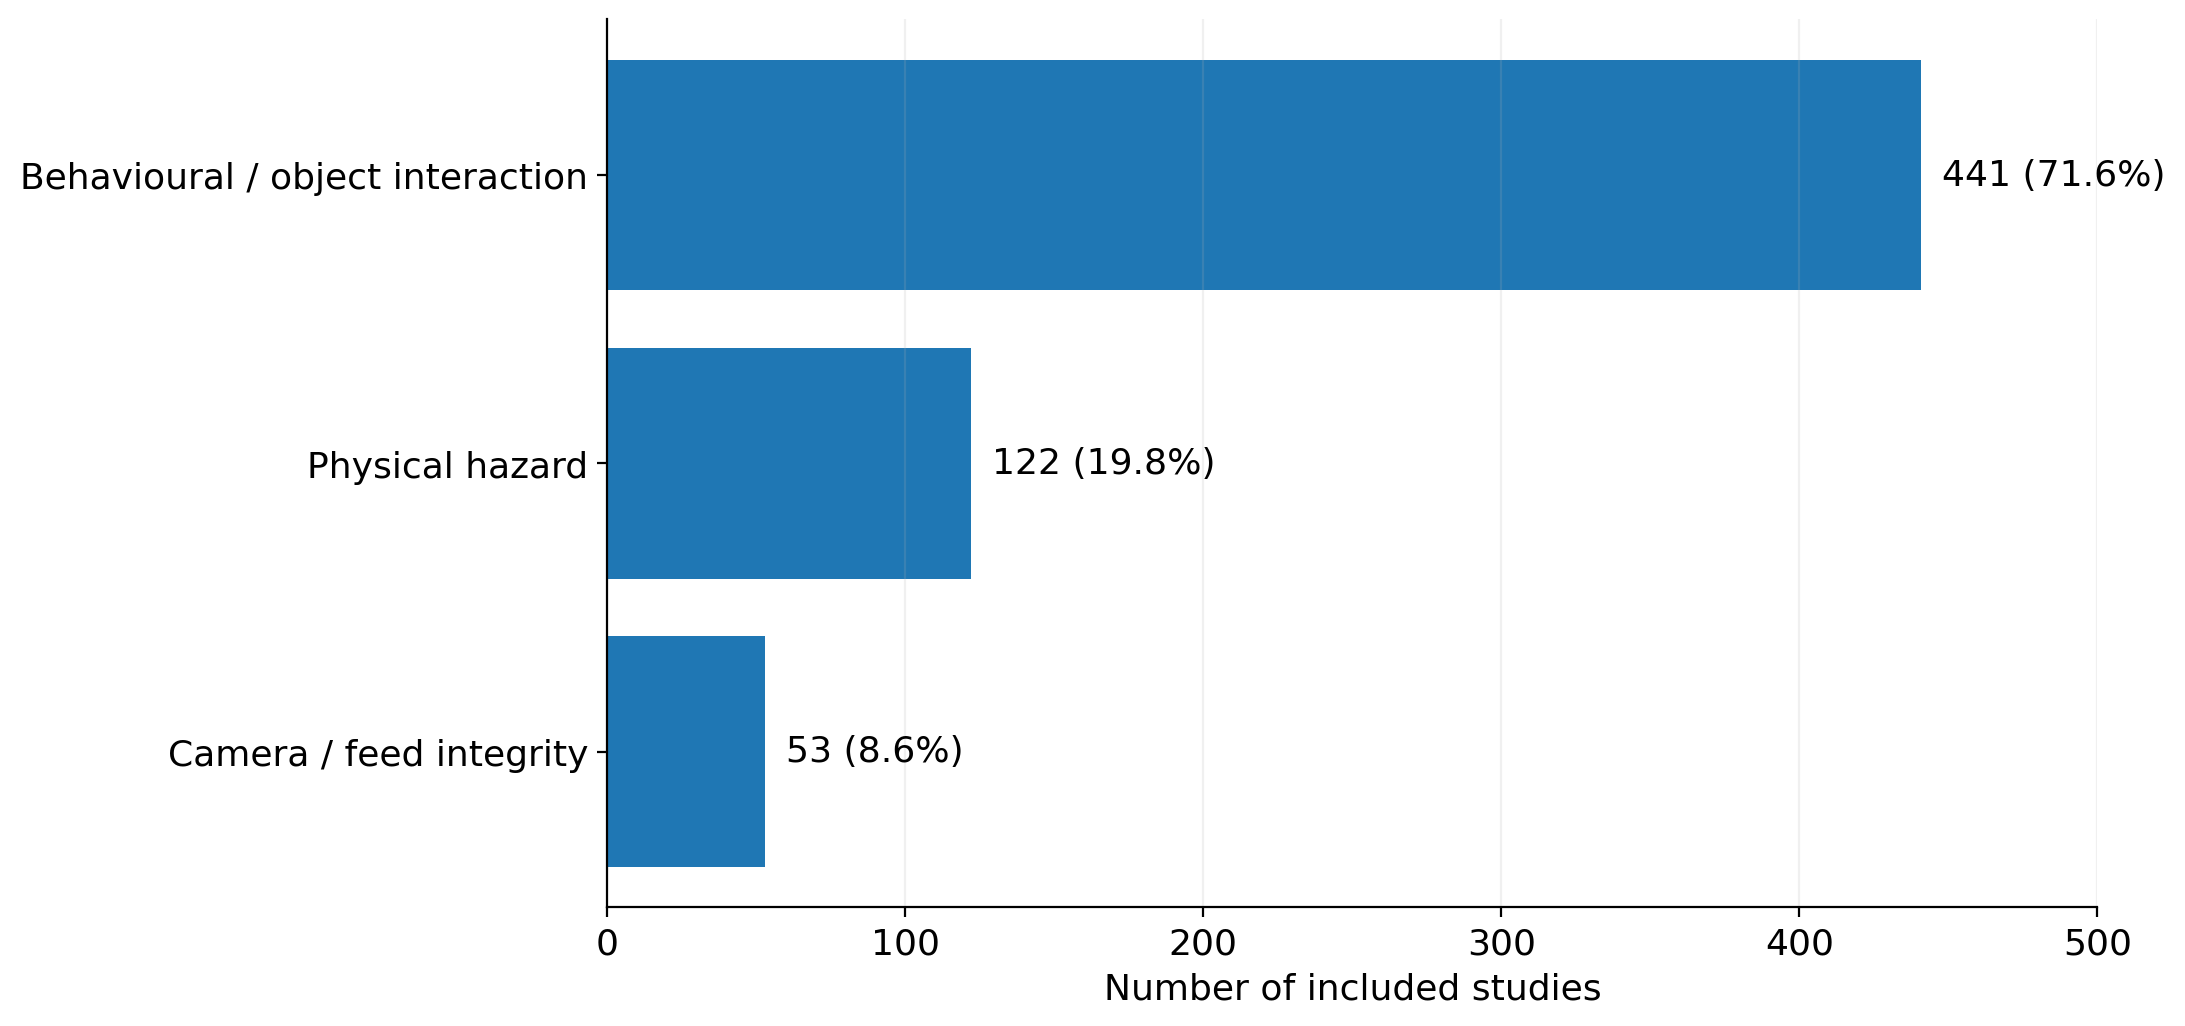
\includegraphics[width=0.86\textwidth]{figure2a_anomaly_category_refined.png}
\caption{Included studies by primary anomaly tier.}\label{fig:tax_a}
\end{subfigure}

\vspace{0.45cm}

\begin{subfigure}{\textwidth}\centering
\begin{tikzpicture}[
  font=\scriptsize,
  root/.style={draw=black!65,fill=black!5,rounded corners=2pt,align=center,inner sep=4pt,font=\scriptsize\bfseries},
  tier/.style={draw=teal!70!black,fill=teal!10,rounded corners=2pt,text width=2.35cm,align=center,inner sep=3pt,font=\scriptsize\bfseries},
  leaf/.style={draw=black!45,fill=white,rounded corners=1.5pt,text width=2.35cm,align=center,inner sep=2.5pt},
  adj/.style={draw=black!40,dashed,fill=black!2,rounded corners=1.5pt,text width=2.35cm,align=center,inner sep=2.5pt},
  ln/.style={draw=black!55,line width=0.5pt},
  dn/.style={draw=black!40,line width=0.5pt,dashed}
]
\node[root] (r) at (0,0) {Visual anomalies\\ in surveillance};
\node[tier] (t1) at (-4.6,-1.15) {Tier 1\\ Behavioural /\\ object interaction};
\node[tier] (t2) at (0,-1.15) {Tier 2\\ Physical hazard};
\node[tier] (t3) at (4.6,-1.15) {Tier 3\\ Camera / feed\\ integrity};
\foreach \z in {t1,t2,t3}{\draw[ln] (r.south) -- (\z.north);}

\foreach \i/\txt in {0/Violent behaviour,1/Suspicious activity,2/Crowd anomaly,3/Fall detection,4/Traffic anomaly,5/Abandoned object}{
  \node[leaf] (a\i) at (-4.6,{-2.15-\i*0.62}) {\txt};}
\foreach \i/\txt in {0/Fire,1/Smoke}{
  \node[leaf] (b\i) at (0,{-2.15-\i*0.62}) {\txt};}
\foreach \i/\txt in {0/Occlusion / tampering,1/Blur / defocus,2/Displacement,3/Freeze / fault}{
  \node[leaf] (c\i) at (4.6,{-2.15-\i*0.62}) {\txt};}
\draw[ln] (t1.south) -- (a0.north);
\foreach \i/\j in {0/1,1/2,2/3,3/4,4/5}{\draw[ln] (a\i.south) -- (a\j.north);}
\draw[ln] (t2.south) -- (b0.north); \draw[ln] (b0.south) -- (b1.north);
\draw[ln] (t3.south) -- (c0.north);
\foreach \i/\j in {0/1,1/2,2/3}{\draw[ln] (c\i.south) -- (c\j.north);}

\node[adj] (adj) at (0,-4.15) {Adjacent phenomena:\\ flooding, explosion,\\ illumination transition};
\draw[dn] (b1.south) -- (adj.north);
\node[draw=black!20,fill=black!2,rounded corners=1.5pt,inner sep=4pt,
      text width=11.2cm,align=center,font=\scriptsize] at (0,-6.35)
  {\textbf{Solid branches} = the twelve core subcategories carried through protocol-level comparison \quad$|$\quad
   \textbf{Dashed branch} = adjacent phenomena, discussed in the review but not protocol-compared};
\end{tikzpicture}
\caption{Operational taxonomy: three tiers and twelve core subcategories.}\label{fig:tax_b}
\end{subfigure}
\caption{Operational taxonomy of visual anomalies in surveillance. Panel~(b) shows the hierarchy: solid branches identify the twelve core subcategories synthesized with protocol-level comparison, and the dashed branch records adjacent phenomena discussed in the review but not treated as directly comparable core categories. Tier~3 covers failures in the complete imaging and transmission pipeline, not only the physical sensor. Panel~(a) reports the working primary-tier allocation for the \pnum{616} included studies: Tier~1 \pnum{441}, Tier~2 \pnum{122}, and Tier~3 \pnum{53}. Studies spanning tiers are assigned to the tier carrying their principal evaluation and should be flagged as multi-category in Supplementary Material~S3. \ifprovisionalnumbers\textbf{The three-tier allocation is a provisional author-review reallocation of the manuscript's earlier multi-category counts and must be verified study by study before submission.}\fi}
\label{fig:taxonomy_tree}
\end{figure*}


\begin{table*}[!t]
\centering
\caption{Operational taxonomy used consistently throughout the review. The twelve core subcategories align with the analytical framework; flooding, explosion, and illumination transitions are discussed as adjacent phenomena because their evidence base is too heterogeneous for separate protocol-level comparison.}
\label{tab:anomaly_taxonomy}
\renewcommand{\arraystretch}{1.28}
\resizebox{\textwidth}{!}{%
\begin{tabular}{p{2.7cm}p{3.6cm}p{5.4cm}p{6.0cm}}
\toprule
\textbf{Tier} & \textbf{Core subcategory} & \textbf{Representative examples} & \textbf{Characteristic evidence} \\
\midrule
\multirow{6}{2.7cm}{\centering Behavioral and object interaction}
& Violent behavior & Fighting, assault, shooting & Rapid pose/motion changes; interaction semantics; crowd response \\
& Suspicious activity & Loitering, trespassing, theft, restricted-area running & Context-dependent dwell time, boundaries, and object interaction \\
& Crowd anomaly & Stampede, congestion, sudden dispersal & Density/flow disruption and coordinated motion change \\
& Fall detection & Slip, collapse, fainting & Upright-to-prone transition and pose trajectory \\
& Traffic anomaly & Wrong-way driving, collision, jaywalking & Trajectory, speed, and lane/context violation \\
& Abandoned object & Unattended bag, package, vehicle & Deposit event followed by persistent non-interaction \\
\midrule
\multirow{2}{2.7cm}{\centering Physical hazard}
& Fire & Indoor, vehicle, and wildfire flames & Color/texture, flicker, expansion, and thermal cues \\
& Smoke & Early smoke, plume, haze & Semi-transparency, diffuse boundaries, upward drift, and low contrast \\
\midrule
\multirow{4}{2.7cm}{\centering Camera and feed integrity}
& Occlusion/tampering & Covered or blocked lens, spray, sticker & Persistent loss of scene content or foreign surface \\
& Blur/defocus & Focus drift, condensation, contamination & Loss of edge sharpness and contrast over time \\
& Displacement & Vandalism, wind, mounting shift & Persistent viewpoint/background change \\
& Freeze/fault & Frozen stream, repeated frames, frame loss, corruption & Temporal stationarity, discontinuity, or transport artifacts \\
\bottomrule
\end{tabular}%
}
\end{table*}


\textbf{Person and scene-related anomalies} constitute the most frequently studied category in the video anomaly detection literature. These anomalies arise from the actions, interactions, or spatial configurations of people and objects within the monitored scene. Violent behavior, including physical altercations, armed aggression, and vandalism, is characterized by abrupt and high-magnitude motion patterns that diverge from the regular flow of pedestrian traffic~\citep{sultani2018real}. Suspicious activities such as loitering, trespassing into restricted zones, and shoplifting involve subtler behavioral deviations that are defined more by spatial and temporal context than by motion magnitude alone~\citep{liu2018future}. Crowd-level anomalies, such as stampedes and sudden dispersal, manifest as large-scale disruptions to the expected density and flow field of pedestrian groups~\citep{li2015crowded}. Fall detection targets sudden transitions from upright to prone posture, which is particularly critical in elderly care and occupational safety settings~\citep{nogas2020deepfall}. Abandoned object detection identifies static foreground entities that persist beyond a contextually appropriate duration~\citep{luna2018abandoned}. Traffic anomalies encompass wrong-way driving, collisions, and pedestrian jaywalking, detectable through trajectory-level reasoning over vehicle and pedestrian tracks~\citep{santhosh2020traffic}.

\textbf{Physical-hazard anomalies} are defined by the observed hazardous phenomenon rather than by whether its real-world cause is natural, accidental, or intentional. Fire detection requires discriminating genuine flame regions from visually similar phenomena such as sunset reflections, emergency lights, and digital signage, a task complicated by the variable and stochastic appearance of combustion~\citep{muhammad2019efficient}. Smoke detection presents additional challenges due to the semi-transparent and amorphous nature of smoke plumes, which lack the well-defined edges that conventional object detectors rely upon~\citep{chen2022fire}. Flooding events alter the ground-plane appearance through reflective water surfaces and progressive occlusion of fixed scene elements~\citep{liang2023vfloodnet}. Explosion detection, while less commonly addressed, involves identifying the transient high-intensity brightness patterns and debris fields associated with blast events~\citep{lopez2018emergency}.

\textbf{Camera and video-feed integrity anomalies}, also referred to in the literature as camera health, camera integrity, or tampering monitoring; we use \emph{camera and video-feed integrity detection} as the umbrella term throughout, affect the imaging pipeline rather than the observed scene. These anomalies are operationally critical because they compromise the reliability of all downstream analysis regardless of its sophistication. Camera occlusion, whether from intentional spray-painting, adhesive stickers, or accidental obstruction, manifests as the partial or complete loss of scene content with the introduction of a static foreign surface~\citep{mantini2019uhctd}. Defocus blur, arising from lens contamination, condensation, or mechanical focus drift, degrades spatial frequency content across the frame or in localized regions~\citep{mantini2017signal}. Camera displacement due to vandalism, strong wind, or mounting instability produces a sudden and persistent change in the observed background scene. Camera freeze, caused by hardware malfunction or network transmission failure, is detectable through the absence of temporal variation across consecutive frames. Illumination anomalies, including sudden artificial lighting changes and day-night infrared mode switching, alter global brightness and color statistics without corresponding changes in scene content~\citep{mantini2023feature_survey}.


\subsection{Deep Learning Architectures for Visual Anomaly Detection}
\label{subsec:dl_architectures}

The evolution of deep learning has introduced a succession of architectural paradigms that have progressively advanced the state of the art in visual anomaly detection. This subsection provides an overview of the principal architecture families, summarized in Table~\ref{tab:architectures}, which serve as the building blocks for the detection methods reviewed in later sections.


\begin{table*}[!t]
\centering
\caption{Overview of deep learning architecture families employed in visual anomaly detection for surveillance, with representative models, typical roles, and principal advantages and limitations.}
\label{tab:architectures}
\renewcommand{\arraystretch}{1.3}
\resizebox{\textwidth}{!}{%
\begin{tabular}{p{3.2cm}p{3.5cm}p{3.5cm}p{3.5cm}p{3.5cm}}
\toprule
\textbf{Architecture Family} & \textbf{Representative Models} & \textbf{Role in Anomaly Detection} & \textbf{Key Advantages} & \textbf{Key Limitations} \\
\midrule
Convolutional Neural Networks (CNNs) & VGG~\citep{simonyan2014very}, ResNet~\citep{he2016deep}, I3D~\citep{carreira2017quo} & Spatial/\hspace{0pt}spatiotemporal feature extraction, classification & Strong spatial inductive bias; well-understood training dynamics; efficient inference & Limited long-range temporal modeling; fixed receptive field \\
\midrule
Recurrent Neural Networks (RNNs) & LSTM~\citep{hochreiter1997long}, GRU~\citep{cho2014learning}, ConvLSTM~\citep{shi2015convolutional} & Temporal sequence modeling, future frame prediction & Natural sequential modeling; memory of past context & Difficulty capturing very long-range dependencies despite gating; sequential computation limits parallelism \\
\midrule
Autoencoders (AEs) & Vanilla AE, VAE~\citep{kingma2013auto}, CAE, MemAE~\citep{gong2019memorizing} & Reconstruction-based normality modeling; latent space learning & Unsupervised training on normal data only; flexible architectures & May reconstruct anomalies well if capacity is too high; blurry reconstructions \\
\midrule
Generative Adversarial Networks (GANs) & DCGAN~\citep{radford2015unsupervised}, WGAN~\citep{arjovsky2017wasserstein}, CycleGAN~\citep{zhu2017unpaired} & Data augmentation; reconstruction-based detection; future prediction & High-fidelity generation; adversarial training sharpens outputs & Training instability; mode collapse; sensitive to hyperparameters \\
\midrule
Diffusion Models (DMs) & DDPM~\citep{ho2020denoising}, LDM~\citep{rombach2022high}, Score-SDE~\citep{song2020score} & Reconstruction-based scoring; anomaly-aware generation & Stable training; superior sample diversity; strong density estimation & High computational cost; slow iterative sampling \\
\midrule
Vision Transformers (ViTs) & ViT~\citep{dosovitskiy2020image}, Swin~\citep{liu2021swin}, TimeSformer~\citep{bertasius2021space}, ViViT~\citep{arnab2021vivit} & Global context modeling; spatiotemporal attention & Captures long-range dependencies; scalable with data; flexible attention patterns & Data-hungry; quadratic attention complexity; less spatial inductive bias \\
\midrule
Graph, Pose, and Normalizing-Flow Models & STG-NF~\citep{hirschorn2023normalizing}, object/pose graphs & Structured actor relations; density estimation on compact representations & Privacy-lean inputs; explicit relational structure; exact likelihood in flow models & Depends on detection/pose quality; weak coverage of non-human hazards \\
\midrule
State-Space Sequence Models & Mamba~\citep{gu2023mamba}, VADMamba~\citep{lyu2025vadmamba} & Long-sequence temporal modeling with linear scaling & Efficient long-context inference; causal implementation is natural & Limited replication and cross-tier evaluation \\
\midrule
Image-Quality and Change-Point Models & BRISQUE~\citep{mittal2012brisque}, NIQE~\citep{mittal2013niqe}, temporal baselines & Feed-quality scoring and abrupt/gradual fault detection & Lightweight, interpretable quality cues; edge-friendly & Camera-specific thresholds; confounding from legitimate scene changes \\
\midrule
Foundation Models (FMs) & CLIP~\citep{radford2021learning}, GPT-4V~\citep{achiam2023gpt}, InternVL~\citep{chen2024internvl}, VideoLLaMA~\citep{zhang2023video} & Zero-shot/few-shot detection; open-vocabulary reasoning; semantic anomaly description & Supports training-free, prompt-tuned, adapter-tuned, or instruction-tuned use; rich cross-modal semantics & High computational requirements; prompt sensitivity; limited fine-grained spatial localization \\
\bottomrule
\end{tabular}%
}
\end{table*}


\textbf{Convolutional Neural Networks.} CNNs have served as the foundational architecture for visual anomaly detection since the mid-2010s. By applying learned convolutional filters in a hierarchical manner, CNNs extract progressively abstract spatial features from raw pixel input, enabling both classification-based and feature-matching-based anomaly detection. Two-dimensional CNNs, such as VGG~\citep{simonyan2014very} and ResNet~\citep{he2016deep}, operate on individual frames or frame pairs, while three-dimensional variants such as C3D~\citep{tran2015learning} and I3D~\citep{carreira2017quo} extend convolution along the temporal axis to capture short-range motion dynamics directly. In the surveillance context, CNNs have been widely employed as backbone feature extractors within both reconstruction-based and classification-based detection pipelines~\citep{sultani2018real, liu2018future}.

\textbf{Recurrent Neural Networks.} RNNs, particularly Long Short-Term Memory (LSTM) networks~\citep{hochreiter1997long} and Gated Recurrent Units (GRUs)~\citep{cho2014learning}, introduce explicit temporal modeling by maintaining a hidden state that evolves across successive time steps. Convolutional LSTM (ConvLSTM)~\citep{shi2015convolutional} combines the spatial feature extraction capacity of convolutions with the sequential memory of recurrence, making it particularly suitable for future frame prediction, a widely adopted proxy task for anomaly detection in which the failure to predict an upcoming frame accurately signals the occurrence of an unexpected event~\citep{liu2018future}. Despite their utility, RNNs suffer from difficulties in capturing very long-range temporal dependencies and from inherently sequential computation that limits training efficiency.

\textbf{Autoencoders.} The autoencoder paradigm, in which an encoder $\mathcal{E}_\phi$ maps input frames to a compressed latent representation $\mathbf{z}$ and a decoder $\mathcal{D}_\psi$ reconstructs the input from $\mathbf{z}$, has become one of the most prevalent frameworks for unsupervised anomaly detection. The core assumption is that an autoencoder trained exclusively on normal data will learn to reconstruct normal patterns faithfully while producing large reconstruction errors for anomalous inputs that fall outside the learned distribution. Variational autoencoders (VAEs)~\citep{kingma2013auto} augment this framework with a probabilistic latent space, enabling density-based anomaly scoring. Memory-augmented autoencoders (MemAE)~\citep{gong2019memorizing} address the undesirable tendency of high-capacity autoencoders to reconstruct anomalies by constraining the reconstruction to draw upon a finite set of prototypical normal patterns stored in an external memory module.

\textbf{Generative Adversarial Networks.} GANs~\citep{goodfellow2014generative} consist of a generator $G$ and a discriminator $D$ trained in an adversarial min-max game, where $G$ learns to produce samples indistinguishable from real data while $D$ learns to differentiate real from generated samples. In anomaly detection, GANs serve a dual purpose: they can generate synthetic anomalous samples to augment scarce training data, and they can function as reconstruction-based detectors by training $G$ to reconstruct normal patterns and using the discriminator score or reconstruction error as an anomaly signal~\citep{ravanbakhsh2017abnormal, liu2018future}. Wasserstein GANs (WGANs)~\citep{arjovsky2017wasserstein} improve training stability through the use of the Earth mover's distance, addressing the mode collapse and gradient instability issues that affect vanilla GAN training.

\textbf{Diffusion Models.} Diffusion models~\citep{ho2020denoising, song2020score} represent the most recent class of generative models to be applied to visual anomaly detection. They operate by learning to reverse a gradual noise-addition process: during training, Gaussian noise is progressively added to data samples over multiple time steps, and a neural network is trained to predict and remove the noise at each step. For anomaly detection, a diffusion model trained on normal data is expected to reconstruct normal inputs with high fidelity while failing to reconstruct anomalous inputs, yielding elevated reconstruction errors. Latent diffusion models (LDMs)~\citep{rombach2022high} perform the diffusion process in a compressed latent space, substantially reducing computational cost while preserving generation quality. The strong density estimation properties and training stability of diffusion models make them an increasingly attractive alternative to GANs for anomaly detection applications.

\textbf{Vision Transformers.} The introduction of the Vision Transformer (ViT)~\citep{dosovitskiy2020image} extended the self-attention mechanism of the Transformer architecture~\citep{vaswani2017attention} to visual data by partitioning images into non-overlapping patches and processing them as token sequences. Unlike CNNs, which rely on local receptive fields, ViTs model global dependencies across all spatial locations through self-attention, enabling the capture of long-range contextual relationships that are critical for understanding scene-level normality. Video-oriented extensions such as TimeSformer~\citep{bertasius2021space}, ViViT~\citep{arnab2021vivit}, and Video Swin Transformer~\citep{liu2022video} extend attention across both spatial and temporal dimensions, providing powerful spatiotemporal representations for video anomaly detection. Hierarchical variants such as the Swin Transformer~\citep{liu2021swin} introduce shifted window attention to achieve linear computational complexity with respect to image resolution, making them practical for high-resolution surveillance analysis.

\textbf{Foundation Models.} Foundation models, encompassing large-scale pretrained vision-language models (VLMs) and large multimodal models (LMMs), represent a recent family of representations and adaptation strategies in visual anomaly detection. CLIP~\citep{radford2021learning}, trained on hundreds of millions of image-text pairs through contrastive learning, enables zero-shot visual recognition by aligning visual and textual embeddings in a shared feature space. For anomaly detection, CLIP-based approaches construct textual descriptions of normal and anomalous conditions and classify video frames based on their similarity to these descriptions, eliminating the need for task-specific labeled training data~\citep{wu2024vadclip, zanella2024harnessing}. More advanced models such as GPT-4V~\citep{achiam2023gpt} and InternVL~\citep{chen2024internvl} can perform visual reasoning over surveillance imagery through natural language interaction, offering interpretable anomaly explanations alongside detection decisions. While these models demonstrate strong generalization capabilities, their computational demands, sensitivity to prompt design, and limited capacity for fine-grained spatial localization remain active areas of investigation.


\subsection{Learning Paradigms}
\label{subsec:learning_paradigms}

The choice of learning paradigm is dictated by the availability and granularity of annotations, which varies considerably across surveillance deployment scenarios. Table~\ref{tab:learning_paradigms} contrasts the principal paradigms along several practically relevant dimensions.


\begin{table*}[!t]
\centering
\caption{Learning regimes used in surveillance anomaly detection. The term ``semi-supervised'' has historically been used inconsistently in VAD; this review uses \emph{normal-only/one-class} for training that contains only normal examples and reserves \emph{semi-supervised} for methods that combine unlabeled/normal data with a small amount of labeled anomaly data.}
\label{tab:learning_paradigms}
\renewcommand{\arraystretch}{1.25}
\resizebox{\textwidth}{!}{%
\begin{tabular}{p{3.1cm}p{4.1cm}p{4.1cm}p{3.0cm}p{5.4cm}}
\toprule
\textbf{Regime} & \textbf{Training information} & \textbf{Typical objective} & \textbf{Label burden} & \textbf{Representative evidence} \\
\midrule
Fully supervised & Frame/pixel/segment labels for normal and anomalous classes & Classification, localization, or segmentation & High & UBnormal supervised open-set protocol~\citep{acsintoae2022ubnormal}; Fine-VAD~\citep{zhang2026finevad} \\
Weakly supervised & Video-level normal/anomalous tags & MIL ranking, feature discrimination, pseudo-label refinement & Moderate & MIL-Rank~\citep{sultani2018real}; RTFM~\citep{tian2021weakly}; VadCLIP~\citep{wu2024vadclip} \\
Semi-supervised & Large unlabeled/normal set plus a small labeled anomaly set & Hybrid one-class and discriminative learning & Low--moderate & Few-shot scene adaptation~\citep{lu2020few} \\
Normal-only / one-class & Normal training data only & Reconstruction, prediction, density, or distance from normality & No anomaly labels & ConvAE~\citep{hasan2016learning}; MemAE~\citep{gong2019memorizing}; MNAD~\citep{park2020learning} \\
Self-supervised & Unlabeled video with automatically generated pretext targets & Temporal order, jigsaw, masked prediction, contrastive learning & None & Multi-task SSL~\citep{georgescu2021anomaly}; SSMTL++~\citep{barbalau2023ssmtl} \\
Training-free zero-shot & Frozen pretrained model plus prompts/rules & Image-text or video-text matching; prompted reasoning & Minimal & LAVAD~\citep{zanella2024harnessing}; AnyAnomaly~\citep{ahn2026anyanomaly}; ASK-HINT~\citep{zou2026askhint} \\
Adapted foundation model & Video labels, learned prompts/adapters, or instruction tuning on top of a foundation model & Weak supervision, prompt learning, alignment, or instruction following & Variable & VadCLIP~\citep{wu2024vadclip}; PEL4VAD~\citep{zhang2024pel4vad}; HAWK~\citep{tang2024hawk}; Alert-CLIP~\citep{zhu2026alertclip} \\
\bottomrule
\end{tabular}%
}
\end{table*}


Fully supervised learning uses dense temporal, spatial, or category labels and is therefore appropriate for closed-set classification or localization when the target classes are predefined. It should not be conflated with the video-level labels used by weakly supervised MIL systems. Weakly supervised learning treats each video as a bag of temporal instances and uses coarse video-level tags, as in MIL-Rank~\citep{sultani2018real}, RTFM~\citep{tian2021weakly}, and later vision-language adaptations such as VadCLIP~\citep{wu2024vadclip}.

Normal-only or one-class learning characterizes the distribution of normality from normal training video and assigns high scores to reconstruction, prediction, density, or representation discrepancies at test time. This regime includes ConvAE, MemAE, MNAD, and many prediction-based methods. Self-supervision is a compatible but distinct mechanism: automatically generated targets such as temporal order, jigsaw reconstruction, masking, or contrastive agreement shape the representation without anomaly labels.

Foundation-model methods span several training regimes rather than forming a single zero-shot category. Frozen CLIP/VLM systems can be training-free, whereas VadCLIP and PEL4VAD use video-level supervision, and HAWK/Alert-CLIP use instruction tuning or representation adaptation. Table~\ref{tab:learning_paradigms} therefore separates training-free use from adapted foundation-model systems.

\subsection{Related Surveys}
\label{subsec:related_surveys}

To position the present work within the broader research landscape, we review prior survey articles that address visual anomaly detection in surveillance and related domains. Table~\ref{tab:survey_comparison} provides a structured comparison of representative surveys along multiple dimensions.


\begin{table*}[!t]
\centering
\caption{Comparison of representative existing surveys on visual anomaly detection. Symbols: \CIRCLE~= comprehensively covered (a dedicated section or systematic treatment with multiple methods/datasets); \LEFTcircle~= partially covered (discussed but not as a primary organizing dimension, or covered for only part of the category); \Circle~= not covered (absent or mentioned only in passing). PA = Person/Scene Anomalies; EA = Environmental Anomalies (fire, smoke, flooding); CA = Camera / Feed Integrity Anomalies; ViT = Vision Transformers; FM = Foundation Models; DP = Deployment and Real-Time Considerations. The final row characterizes the present review against the same criteria; as a self-assessment it is provided for transparency of scope rather than as an independent quality judgment.}
\label{tab:survey_comparison}
\renewcommand{\arraystretch}{1.3}
\resizebox{\textwidth}{!}{%
\begin{tabular}{llccccccccc}
\toprule
\textbf{Reference} & \textbf{Year} & \textbf{Venue} & \multicolumn{3}{c}{\textbf{Anomaly Coverage}} & \multicolumn{4}{c}{\textbf{Methodology Coverage}} & \textbf{DP} \\
\cmidrule(lr){4-6} \cmidrule(lr){7-10}
 & & & PA & EA & CA & CNN/RNN & GAN/AE & ViT & FM & \\
\midrule
Ramachandra et al.~\citeyearpar{ramachandra2020survey} & 2020 & IEEE TPAMI & \CIRCLE & \Circle & \Circle & \CIRCLE & \CIRCLE & \Circle & \Circle & \LEFTcircle \\
Santhosh et al.~\citeyearpar{santhosh2020traffic} & 2020 & ACM CSUR & \LEFTcircle & \Circle & \Circle & \CIRCLE & \LEFTcircle & \Circle & \Circle & \LEFTcircle \\
Chandrakala et al.~\citeyearpar{chandrakala2023thematic} & 2023 & Artif. Intell. Rev. & \CIRCLE & \Circle & \Circle & \CIRCLE & \CIRCLE & \LEFTcircle & \Circle & \LEFTcircle \\
Nayak et al.~\citeyearpar{nayak2021comprehensive} & 2021 & Image Vis. Comput. & \CIRCLE & \Circle & \Circle & \CIRCLE & \CIRCLE & \Circle & \Circle & \LEFTcircle \\
Rezaee et al.~\citeyearpar{rezaee2021crowd_realtime} & 2024 & Pers. Ubiquit. Comput. & \CIRCLE & \Circle & \Circle & \CIRCLE & \LEFTcircle & \Circle & \Circle & \CIRCLE \\
Sharif et al.~\citeyearpar{sharif2022deep_crowd} & 2022 & arXiv & \CIRCLE & \Circle & \Circle & \CIRCLE & \CIRCLE & \LEFTcircle & \Circle & \Circle \\
Wang et al.~\citeyearpar{wang2022deep_fire} & 2022 & Neurocomputing & \Circle & \CIRCLE & \Circle & \CIRCLE & \LEFTcircle & \LEFTcircle & \Circle & \LEFTcircle \\
Patrikar and Parate~\citeyearpar{patrikar2022anomaly} & 2022 & Int. J. Multimed. Inf. Retr. & \CIRCLE & \Circle & \Circle & \CIRCLE & \CIRCLE & \LEFTcircle & \Circle & \LEFTcircle \\
Mantini and Shah~\citeyearpar{mantini2023feature_survey} & 2023 & arXiv & \Circle & \Circle & \CIRCLE & \LEFTcircle & \Circle & \Circle & \Circle & \LEFTcircle \\
Tran et al.~\citeyearpar{tran2024anomaly_images_videos} & 2024 & ACM CSUR & \CIRCLE & \Circle & \Circle & \CIRCLE & \CIRCLE & \CIRCLE & \LEFTcircle & \Circle \\
Wu et al.~\citeyearpar{wu2024deep_review} & 2026 & IEEE TNNLS & \CIRCLE & \Circle & \Circle & \CIRCLE & \CIRCLE & \CIRCLE & \LEFTcircle & \LEFTcircle \\
Saleh et al.~\citeyearpar{saleh2024forest_fire} & 2024 & Heliyon & \Circle & \CIRCLE & \Circle & \CIRCLE & \LEFTcircle & \LEFTcircle & \Circle & \LEFTcircle \\
Ren et al.~\citeyearpar{ren2025foundation_anomaly} & 2025 & AI Magazine & \LEFTcircle & \Circle & \Circle & \LEFTcircle & \LEFTcircle & \CIRCLE & \CIRCLE & \LEFTcircle \\
Ben Ammar et al.~\citeyearpar{benammar2025foundation_transformer} & 2025 & Inf. Fusion & \LEFTcircle & \Circle & \Circle & \LEFTcircle & \LEFTcircle & \CIRCLE & \CIRCLE & \Circle \\
Song et al.~\citeyearpar{song2024networking_vad} & 2025 & ACM CSUR & \CIRCLE & \Circle & \Circle & \CIRCLE & \CIRCLE & \CIRCLE & \LEFTcircle & \CIRCLE \\
Noghre et al.~\citeyearpar{noghre2025survey_human_vehicle} & 2025 & arXiv & \CIRCLE & \LEFTcircle & \Circle & \CIRCLE & \CIRCLE & \CIRCLE & \LEFTcircle & \LEFTcircle \\
Gaur et al.~\citeyearpar{gaur2025early_fire_smoke} & 2025 & Applied Sciences & \Circle & \CIRCLE & \Circle & \CIRCLE & \LEFTcircle & \CIRCLE & \LEFTcircle & \LEFTcircle \\
Zhu et al.~\citeyearpar{zhu2026generative} & 2026 & Artif. Intell. Rev. & \LEFTcircle & \Circle & \Circle & \CIRCLE & \CIRCLE & \CIRCLE & \CIRCLE & \LEFTcircle \\
\bottomrule
\end{tabular}%
}
\end{table*}


Several patterns emerge from this comparison that collectively motivate the present work. The majority of prior surveys concentrate on person- and scene-related anomalies, with fire and smoke detection treated as a separate subfield and camera/video-feed-integrity anomalies addressed only in a handful of narrow-scope reviews. Within the reviewed literature, we did not identify a surveillance-focused survey that combines all three anomaly categories with the same taxonomy--method coverage analysis. Furthermore, while convolutional and recurrent architectures are well represented, foundation model-based detection receives substantive attention only in domain-general reviews that extend well beyond surveillance. Deployment considerations receive at most partial attention in most existing works.

It is important to differentiate the present work from four categories of closely related recent surveys. First, \emph{surveillance-focused VAD reviews} such as Tran et al.~\citeyearpar{tran2024anomaly_images_videos}, and Song et al.~\citeyearpar{song2024networking_vad} provide thorough coverage of person/scene anomaly detection methods but do not treat fire/smoke or camera/video-feed-integrity anomalies as first-class categories, and their coverage of foundation models remains partial. Second, \emph{foundation-model-centric reviews} by Ren et al.~\citeyearpar{ren2025foundation_anomaly} and Ben Ammar et al.~\citeyearpar{benammar2025foundation_transformer} provide excellent architectural coverage of vision-language models but span industrial, medical, and surveillance domains without the surveillance-specific depth or three-tier anomaly taxonomy that we develop. Third, this journal has previously published a thematic taxonomy of deep models for surveillance video anomaly detection~\citep{chandrakala2023thematic}. That review organises the field by model family within a single anomaly domain (person- and scene-level events) and reports a comparative performance analysis across those models. The present review differs on the dimension that defines it: it treats physical hazards and camera/video-feed integrity as co-equal analytical tiers rather than as out-of-scope subfields, and it codes supervision, scoring, and representation as separable dimensions rather than resolving each method into a single model-family bin. Fourth, the concurrent survey by Zhu et al.~\citeyearpar{zhu2026generative}, published in \emph{Artificial Intelligence Review} (2026), reviews generative anomaly detection comprehensively, spanning autoencoders, GANs, diffusion models, and foundation models, but organizes the literature by generative paradigm rather than by surveillance anomaly category. It does not cover fire/smoke detection or camera/video-feed-integrity anomalies as distinct analytical targets, and its scope extends well beyond surveillance into industrial and medical domains. The present survey addresses a complementary gap: a surveillance-specific, dual-axis review that treats anomaly taxonomy and computational methodology as equal organizing dimensions, enabling the cross-category transferability analysis and deployment-oriented synthesis that single-axis reviews cannot provide. Concretely, existing surveillance-focused surveys rarely treat fire/smoke and camera/feed integrity as co-equal analytical targets, and domain-general foundation-model surveys do not provide surveillance-specific treatment of feed failure, operational metrics, or cross-tier transfer. The present review therefore addresses a complementary gap through an operational three-tier taxonomy and protocol-aware comparison.


%% ===========================================================================
%% NEW SECTION: Proposed Dual-Axis Analytical Framework
%% ===========================================================================

\section{Operational Analytical Framework}
\label{sec:framework}

This section introduces a two-axis framework that separates \emph{what deviates} from \emph{how deviation is modeled}. The purpose is analytical clarity rather than a numerical ranking of heterogeneous studies.

\subsection{Framework Overview}
\label{subsec:framework_overview}
The first axis is the operational anomaly tier: behavioral/object interaction, physical hazard, or camera/video-feed integrity. The second axis is decomposed into three separable dimensions: supervision regime, scoring mechanism, and representation family. A study can therefore be weakly supervised, use a transformer representation, and optimize a MIL ranking score simultaneously; none of these labels excludes the others. Figure~\ref{fig:framework} depicts this two-axis organization and its supporting operational fields (output granularity and deployment profile), and the worked example within it shows how a single study occupies several dimensions at once, the visual counterpart to the coding vocabulary formalized in Table~\ref{tab:orthogonal_coding}.

\begin{figure*}[!t]
\centering
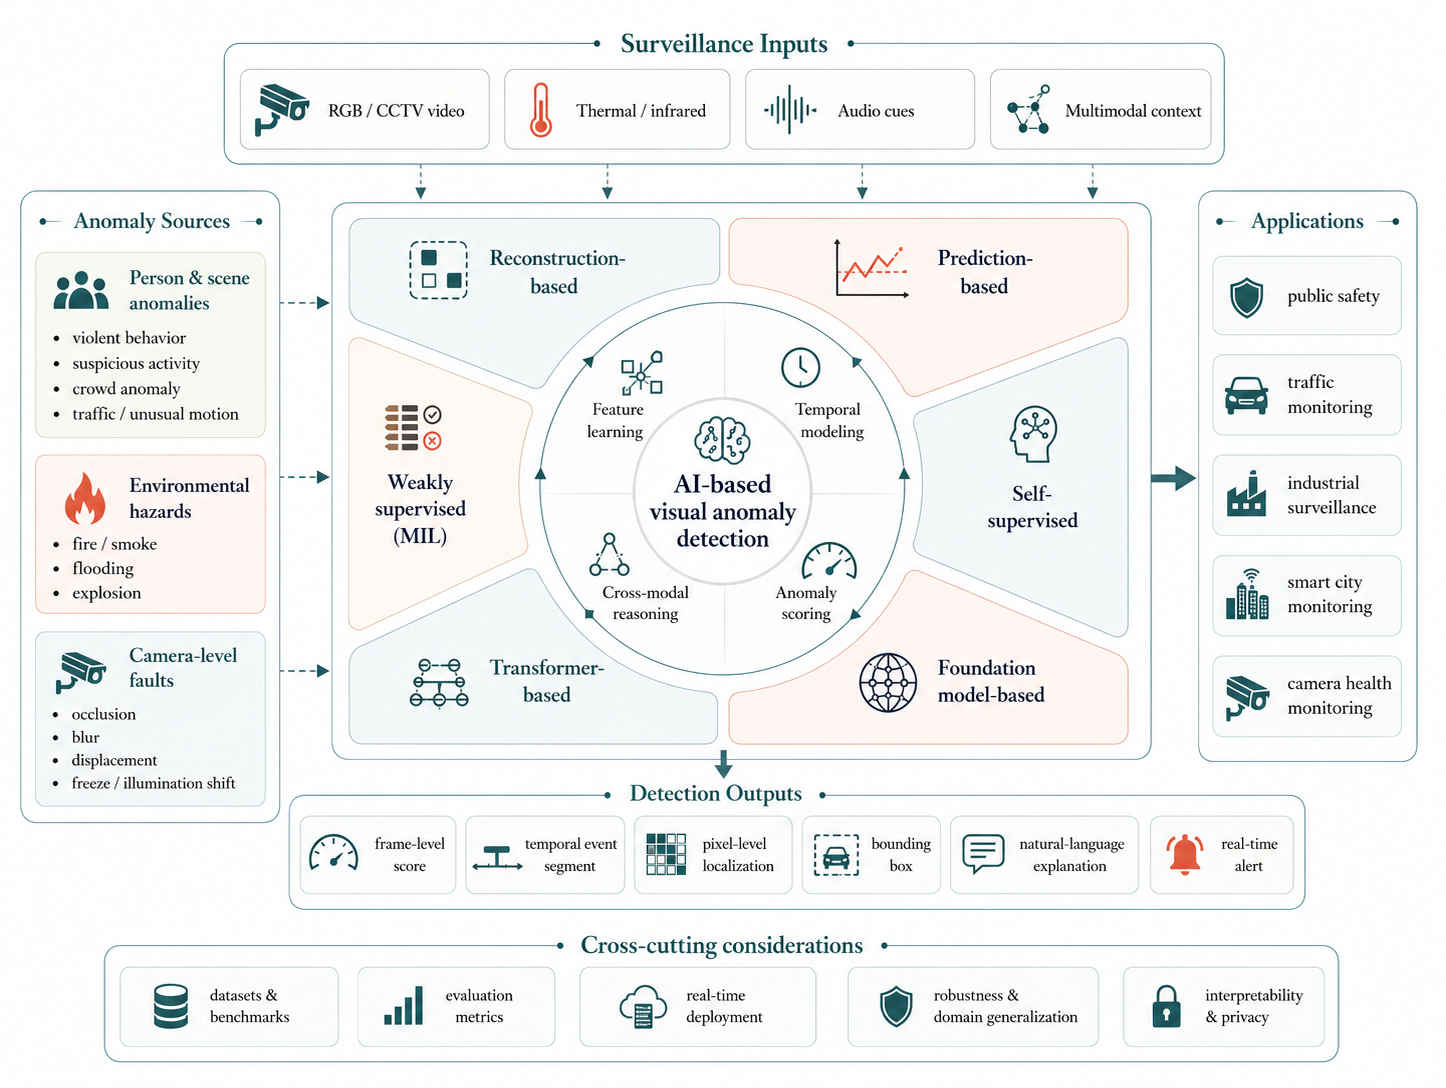
\includegraphics[width=\textwidth]{framework_diagram.png}
\caption{Separable analytical framework used in the review. Anomaly tier describes what deviates; training information, anomaly evidence, and representation describe how the detector is constructed; output and deployment fields describe how the result is delivered and evaluated. The worked example demonstrates why a single paper can occupy several dimensions simultaneously.}
\label{fig:framework}
\end{figure*}

\subsection{Axis 1: Operational Anomaly Taxonomy}
\label{subsec:axis1}
The twelve core subcategories in Table~\ref{tab:anomaly_taxonomy} are used consistently in the rest of the review. Tier~1 requires contextual motion, pose, object-interaction, or trajectory reasoning. Tier~2 emphasizes photometric, textural, thermal, and temporal signatures of combustion phenomena. Tier~3 requires image-quality, background-consistency, change-point, and stream-integrity monitoring. The tier labels describe the detection problem rather than uncertain real-world causality.

\subsection{Axis 2: Separable Method Dimensions}
\label{subsec:axis2}
The second analytical axis is intentionally decomposed because common VAD labels describe different ontological properties. A \emph{supervision regime} specifies the information available during training or adaptation; an \emph{anomaly-scoring mechanism} specifies the quantity interpreted as evidence of abnormality; and a \emph{representation family} specifies the feature or temporal backbone that produces that evidence. Output granularity and deployment profile are recorded as additional operational dimensions. These properties are not mutually exclusive and should not be collapsed into a single method category.

Multi-label coding is applied conservatively. A study receives a supervision code when that information is used to fit or adapt the model; it receives a scoring code when the corresponding quantity directly contributes to the test-time anomaly decision; and it receives a representation code when the architecture produces features or temporal context used by that decision. Merely citing a transformer, using CLIP features as an unmodified preprocessing step, or reporting an auxiliary reconstruction loss is not sufficient to assign every possible label. The coding therefore represents the operational decision pathway rather than the vocabulary used in a paper's title.

For example, VadCLIP~\citep{wu2024vadclip} is coded as video-level weak supervision in the first dimension, discriminative and prompt-similarity scoring in the second, and a CLIP/transformer representation in the third. Its output is a temporal frame/segment score, while its deployment profile is offline evaluation with frozen visual-language features rather than training-free zero-shot inference. By contrast, STG-NF~\citep{hirschorn2023normalizing} is normal-only, uses density/likelihood scoring, and operates on pose-graph representations with a normalizing-flow model; it is not a transformer method. This separation is used throughout Sections~\ref{sec:sota}--\ref{sec:datasets} to prevent architecture, supervision, and anomaly evidence from being interpreted as competing single-axis paradigms.

Table~\ref{tab:orthogonal_coding} defines the coding vocabulary. The machine-readable extraction table contains one row per study--dataset--metric result, allowing a paper to receive multiple legitimate codes without generating an artificial Cartesian product of every label.

\begin{table*}[!t]
\centering
\caption{Separable method dimensions used to describe the reviewed evidence. A paper may receive multiple codes within and across dimensions.}
\label{tab:orthogonal_coding}
\renewcommand{\arraystretch}{1.3}
\resizebox{\textwidth}{!}{%
\begin{tabular}{p{3.5cm}p{7.1cm}p{7.0cm}}
\toprule
\textbf{Dimension} & \textbf{Codes} & \textbf{Interpretive question} \\
\midrule
Supervision regime & Fully supervised; weakly supervised; semi-supervised; normal-only/one-class; self-supervised; training-free zero-shot; few-shot/adapted FM & What information is available during training or adaptation? \\
Anomaly-scoring mechanism & Reconstruction error; future/flow prediction error; density/distance; discriminative/MIL score; prompt similarity; teacher-student discrepancy; rule violation; change-point/quality score & What quantity is treated as evidence of abnormality? \\
Representation family & Handcrafted/IQA; 2D/3D CNN; RNN/ConvLSTM; graph/pose; transformer; state-space model; vision-language or multimodal foundation model & Which representation or temporal backbone produces the evidence? \\
Output granularity & Frame score; temporal event; bounding box/tube; pixel mask; category label; natural-language description & What action-relevant output is produced? \\
Deployment profile & Offline/online; causal/bidirectional; RGB/audio/thermal; edge/cloud; parameters/FLOPs/FPS/latency; privacy mode & Under which operational conditions was the system evaluated? \\
\bottomrule
\end{tabular}%
}
\end{table*}

\subsection{Evidence Maturity Across Tiers}
\label{subsec:evidence_maturity}
Instead of a pseudo-precise count matrix whose values depend on overlapping coding decisions, Table~\ref{tab:evidence_maturity} applies predeclared maturity criteria. \emph{Mature} requires at least three reusable public benchmarks, at least five independent method families, and repeated protocol-level comparisons by different groups. \emph{Established} requires at least one reusable public benchmark and at least three independently evaluated method families. \emph{Emerging} denotes more than one independent study but limited benchmark diversity or replication. \emph{Sparse} denotes isolated demonstrations or evidence dominated by proprietary/custom corpora. These thresholds describe evidence infrastructure, not effect size or model quality.

\begin{table*}[!t]
\centering
\caption{Evidence maturity by operational tier. The labels summarize benchmark availability, method diversity, replication, and operational reporting; they are not effect-size estimates.}
\label{tab:evidence_maturity}
\renewcommand{\arraystretch}{1.3}
\resizebox{\textwidth}{!}{%
\begin{tabular}{p{3.2cm}p{3.0cm}p{5.3cm}p{6.5cm}}
\toprule
\textbf{Tier} & \textbf{Maturity} & \textbf{Evidence basis} & \textbf{Principal unresolved weakness} \\
\midrule
Behavioral/object interaction & Mature for frame-level VAD; established for event/localization tasks & Multiple public datasets (Ped2, Avenue, ShanghaiTech, UCF-Crime, XD-Violence, Street Scene, UBnormal, NWPU Campus, CHAD) and all major learning regimes & Cross-scene generalization, low-FPR recall, event localization, and controlled comparison across backbones/pretraining \\
Fire and smoke hazards & Established for classification/detection; emerging for open-vocabulary and early-event evaluation & Public image/video corpora and mature object-detection/segmentation architectures & Task/metric fragmentation, false alarms from fog/steam/reflections, and limited early-detection latency reporting \\
Camera/video-feed integrity & Emerging for tampering; sparse for gradual degradation and transport faults & UHCTD and a small number of custom or mixed corpora; handcrafted, IQA, and limited learned methods & Cross-camera/season validation, gradual faults, false alarms per camera hour, and modern self-supervised/foundation baselines \\
Unified multi-tier systems & Sparse & A few mixed datasets and open-world systems, but no standard benchmark spanning all three tiers & No common training/evaluation protocol and no evidence that one architecture is reliable across all tiers \\
\bottomrule
\end{tabular}%
}
\end{table*}

\subsection{Mechanism-Level Transfer Assessment}
\label{subsec:transfer_assessment}
Cross-tier transfer is assessed through five questions rather than through author-assigned numerical priors:
\begin{enumerate}
    \item Does the source representation preserve the target tier's discriminative visual/temporal cues?
    \item Can the normality or class model be re-estimated without dense target annotations?
    \item Does the source anomaly score encode a target-compatible assumption?
    \item Are target-tier confounders represented in training and validation data?
    \item Is performance evaluated using target-appropriate operational metrics?
\end{enumerate}

Table~\ref{tab:transfer_roadmap} applies these five questions to each candidate source mechanism, recording the redesign a transfer would require, the evidence that would validate it, and the current evidential status of the claim. The entries are stated as hypotheses (formalized as H1--H5 in Section~\ref{subsec:critical_synthesis}) rather than as measured transfer scores.

\begin{table*}[!t]
\centering
\caption{Cross-tier transfer hypotheses and the evidence required to validate them. These are research hypotheses, not measured transfer scores.}
\label{tab:transfer_roadmap}
\renewcommand{\arraystretch}{1.25}
\resizebox{\textwidth}{!}{%
\begin{tabular}{p{3.2cm}p{2.2cm}p{4.5cm}p{5.0cm}p{3.3cm}}
\toprule
\textbf{Source mechanism} & \textbf{Target tier} & \textbf{Required redesign} & \textbf{Validation evidence} & \textbf{Current evidence status} \\
\midrule
Reconstruction and feature prediction & Feed integrity & Per-camera adaptive baseline; quality-sensitive representation; abrupt and gradual score components & Cross-camera/day--night tests, gradual blur/occlusion trajectories, camera-hour false alarms, detection delay & Adjacent-domain evidence; no replicated cross-tier experiment \\
Self-supervised pretexts & Feed integrity & Blur, exposure, compression, and frame-order tasks that decouple scene change from feed failure & Real and synthetic faults, unseen cameras, seasonal drift, NR-IQA/change-point ablations & Isolated components; integrated validation remains sparse \\
Weakly supervised MIL & Fire and smoke & Replace generic feature-magnitude ranking with regional, photometric, and temporal evidence & Smoke-only recall, early-event latency, confounder sets, localization and low-FPR evaluation & Hypothesis; direct MIL-to-smoke transfer not established \\
Vision-language models & Fire and smoke & Fine-grained combustion prompts, temporal aggregation, small-region grounding, calibrated abstention & Cross-weather/day--night tests, prompt robustness, localization, false-alarm and calibration analysis & Early open-vocabulary evidence; limited early-smoke validation \\
Vision-language models & Feed integrity & Sensor-fault vocabulary, temporal references, evidence-grounded description & Public benchmark with unseen fault descriptions, cross-camera transfer, faithfulness and latency & No public unified benchmark \\
\bottomrule
\end{tabular}%
}
\end{table*}

\subsection{Multi-Tier and Unified Evidence}
\label{subsec:multi_tier}
The literature uses \emph{multi-category} and \emph{multi-tier} inconsistently. UCF-Crime contains behavioral categories together with arson and explosion, but it does not evaluate camera/feed failure. ADOC~\citep{doshi2022adoc} is more directly multi-tier because it combines scene anomalies with camera tampering. Open-world systems such as HAWK~\citep{tang2024hawk}, AnyAnomaly~\citep{ahn2026anyanomaly}, ASK-HINT~\citep{zou2026askhint}, and LAVIDA~\citep{dai2026lavida} broaden anomaly vocabulary, yet their published evaluations remain concentrated on behavioral VAD. LAS-VAD~\citep{wang2026lasvad} incorporates semantic attributes such as flame and smoke when reasoning about behavioral anomaly classes, but it is not a joint fire-monitoring and camera-health system. The evidence therefore supports modular or open-vocabulary multi-category analysis, not a validated single architecture that jointly detects behavioral events, physical hazards, and feed failures under one protocol.

\begin{table*}[!t]
\centering
\caption{Representative multi-category or multi-tier evidence. The table distinguishes dataset breadth from validated joint operation across all three tiers.}
\label{tab:multi_tier_evidence}
\renewcommand{\arraystretch}{1.22}
\resizebox{\textwidth}{!}{%
\begin{tabular}{p{3.0cm}p{4.2cm}p{4.4cm}p{6.0cm}}
\toprule
\textbf{Evidence} & \textbf{Coverage} & \textbf{What is jointly evaluated} & \textbf{Limitation} \\
\midrule
UCF-Crime~\citep{sultani2018real} & Behavioral categories plus arson/explosion labels & Weakly supervised temporal scoring within one dataset & No camera/feed-failure evaluation; physical hazards are not assessed under early-warning protocols \\
ADOC~\citep{doshi2022adoc} & Scene anomalies and camera tampering & Online anomaly scoring in a mixed campus corpus & Small study-specific protocol; does not cover fire/smoke \\
HAWK / VADER~\citep{tang2024hawk,cheng2026vader} & Open-world anomaly description and relation-aware understanding & Behavioral detection plus semantic description & Published evaluation remains behavior-centric; description quality is not joint tier reliability \\
AnyAnomaly / ASK-HINT / LAVIDA~\citep{ahn2026anyanomaly,zou2026askhint,dai2026lavida} & User-defined or zero-shot anomaly vocabulary & Cross-dataset behavioral VAD and reasoning & No standard feed-integrity or early-hazard benchmark \\
Modular deployment proposed in this review & Behavioral, hazard, and feed-integrity modules & Shared event aggregation, calibration, explanation, and operator interface & Research architecture; requires prospective multi-camera validation \\
\bottomrule
\end{tabular}%
}
\end{table*}

\section{State of the Art in Visual Anomaly Detection}
\label{sec:sota}

This section provides a detailed analysis of the current state of the art in visual anomaly detection for surveillance, organized along the anomaly taxonomy axis of our proposed framework. For each anomaly category, we identify the leading methods, analyze performance trajectories over time, and discuss the methodological factors that have driven recent advances. This section complements the methodology-centric review in Section~\ref{sec:methods} by providing a category-centric perspective that reveals which computational approaches have proven most effective for each specific type of visual anomaly.


\subsection{State of the Art in Person and Scene Anomaly Detection}
\label{subsec:sota_person}

Person- and scene-related anomaly detection has witnessed the most rapid methodological progression, benefiting from the availability of multiple large-scale benchmarks and sustained community interest. Table~\ref{tab:sota_person} presents selected historical milestones and explicitly records the training regime associated with each result.

\begin{table*}[!t]
\centering
\caption{Selected historical milestones on canonical VAD benchmarks. Values are literature-reported frame-level AUC (\%) and are not a controlled leaderboard: direct comparison requires a matched training regime, features, preprocessing, and evaluation code. A dash (--) indicates that the cited study does not report a result on that benchmark. Because the table mixes supervision regimes (normal-only Ped2/Avenue/ShanghaiTech AUC with weakly supervised UCF-Crime AUC), rows must not be read as a single performance trajectory across columns. Some legacy baselines are reproduced from later comparative tables when the original publication used a different reporting layout; the canonical consolidated comparisons are Tables~\ref{tab:consolidated_performance} and~\ref{tab:weak_foundation_performance}, and Supplementary Material~S4 records the immediate numerical source.}
\label{tab:sota_person}
\renewcommand{\arraystretch}{1.2}
\resizebox{\textwidth}{!}{%
\begin{tabular}{c p{3.1cm} p{3.0cm} c c c c p{3.0cm} p{4.6cm}}
\toprule
\textbf{Year} & \textbf{Method} & \textbf{Training regime} & \textbf{Ped2} & \textbf{Avenue} & \textbf{SHTech} & \textbf{UCF-Crime} & \textbf{Representation} & \textbf{Contribution} \\
\midrule
2016 & Conv-AE~\citep{hasan2016learning} & Normal-only & 85.0 & 80.0 & 60.9 & -- & ConvAE & End-to-end reconstruction baseline \\
2018 & Frame-Pred~\citep{liu2018future} & Normal-only & 95.4 & 85.1 & 72.8 & -- & U-Net + GAN & Multi-loss future-frame prediction \\
2018 & MIL-Rank~\citep{sultani2018real} & Video-level weak supervision & -- & -- & -- & 75.4 & C3D & Large-scale MIL formulation and UCF-Crime \\
2019 & MemAE~\citep{gong2019memorizing} & Normal-only & 94.1 & 83.3 & 71.2 & -- & AE + memory & Prototype-constrained reconstruction \\
2020 & MNAD~\citep{park2020learning} & Normal-only & 97.0 & 88.5 & 70.5 & -- & AE + memory & Reconstruction and prediction memory branches \\
2021 & RTFM~\citep{tian2021weakly} & Video-level weak supervision & -- & -- & 97.2 & 84.3 & I3D & Top-$k$ feature-magnitude learning \\
2021 & Georgescu et al.~\citeyearpar{georgescu2021anomaly} & Self-supervised & 97.8 & 89.3 & 82.7 & -- & Multi-task CNN & Multiple temporal pretext tasks \\
2023 & SSMTL++v1~\citep{barbalau2023ssmtl} & Self-supervised & -- & 93.7 & 82.9 & -- & Multi-task + CvT/pretexts & Variant-specific multi-task normality learning \\
2023 & STG-NF~\citep{hirschorn2023normalizing} & Normal-only / pose & -- & -- & 85.9 & -- & Pose + normalizing flow & Privacy-lean structured density modeling \\
2023 & FPDM~\citep{yan2023feature} & Normal-only & -- & 90.1 & 78.6 & -- & Feature diffusion & Diffusion-based feature prediction \\
2024 & VadCLIP~\citep{wu2024vadclip} & Video labels + frozen CLIP & -- & -- & -- & 88.0 & CLIP ViT-B/16 & Vision-language adaptation evaluated on UCF-Crime and XD-Violence \\
\bottomrule
\end{tabular}%
}
\end{table*}


The trajectory reveals four distinct eras of progress. The \textit{reconstruction era} (2016--2019) established deep autoencoders as the foundational paradigm, with performance on Ped2 climbing from 85.0\% to 97.0\% through architectural innovations including memory modules and prediction branches. The \textit{prediction and supervision era} (2018--2021) introduced complementary advances through future frame prediction and weakly supervised MIL, with the latter substantially advancing large-scale, diverse-category detection on UCF-Crime. The \textit{self-supervised and transformer era} (2021--2023) reported strong results on normal-only and self-supervised benchmarks through multi-task pretext learning and attention-based architectures, while also introducing skeleton-based methods that decouple anomaly detection from appearance-level features. The \textit{foundation model era} (2024--present) has reported strong results on weakly supervised benchmarks under language-adapted protocols through vision-language alignment. VadCLIP, for example, reports 88.0\% AUC on UCF-Crime and 84.5\% AP on XD-Violence (as reported; consistent with Tables~\ref{tab:sota_person}, \ref{tab:foundation_methods}, and~\ref{tab:weak_foundation_performance}), compared with 75.4\% UCF-Crime AUC for the original C3D-based MIL baseline. This gain, however, confounds paradigm with backbone and pretraining scale (CLIP ViT-B vs.\ C3D) and should be read as indicative of a promising direction rather than as a controlled comparison (see Section~\ref{subsec:critical_synthesis}).


\subsection{State of the Art in Fire and Smoke Detection}
\label{subsec:sota_fire}

The state of the art in visual fire and smoke detection has progressed along a trajectory that parallels the broader evolution of object detection architectures, from two-stage region proposal networks through single-stage detectors to attention-enhanced and transformer-based architectures. Because this literature spans three distinct task formulations, the evidence is tabulated in two blocks that must not be read across: Table~\ref{tab:sota_fire_classification} reports whole-image classification accuracy, while Table~\ref{tab:sota_fire_detection} reports detection mAP and segmentation mIoU, whose thresholds and test splits are set by each originating study.

\begin{table*}[!t]
\centering
\caption{Representative visual fire/smoke classification studies. Accuracy values are dataset-specific and should not be compared across corpora without matched splits. $^{\dagger}$Preprint-only source; its reported accuracy is recorded for completeness and, consistent with the evidence policy of Section~\ref{subsec:eligibility}, is not used to support any comparative or state-of-the-art claim.}
\label{tab:sota_fire_classification}
\renewcommand{\arraystretch}{1.2}
\resizebox{\textwidth}{!}{%
\begin{tabular}{c p{3.3cm} p{3.1cm} p{3.4cm} p{2.5cm} p{6.0cm}}
\toprule
\textbf{Year} & \textbf{Study} & \textbf{Architecture} & \textbf{Evaluation corpus} & \textbf{Reported metric} & \textbf{Contribution / caveat} \\
\midrule
2015 & Foggia et al.~\citeyearpar{foggia2015fire} & Multi-expert CNN & Surveillance videos & 93.5\% accuracy & Early real-time video fire classifier; corpus-specific protocol \\
2019 & Muhammad et al.~\citeyearpar{muhammad2019efficient} & Fine-tuned SqueezeNet & Custom CCTV & 94.5\% accuracy & Lightweight surveillance-oriented model \\
2019 & FireNet$^{\dagger}$~\citep{jadon2019firenet} & Compact CNN & FireNet & 95.2\% accuracy & Edge-oriented classifier; limited dataset diversity \\
2022 & Huang et al.~\citeyearpar{chen2022fire} & Wavelet + CNN & Benchmark image and video sets & 96.8\% accuracy & Spectral features reduce some fire-like false alarms \\
\bottomrule
\end{tabular}%
}
\end{table*}

\begin{table*}[!t]
\centering
\caption{Representative fire/smoke detection and segmentation studies. Metrics are shown within task type only; mAP thresholds and test splits depend on the original study protocols.}
\label{tab:sota_fire_detection}
\renewcommand{\arraystretch}{1.2}
\resizebox{\textwidth}{!}{%
\begin{tabular}{c p{3.1cm} p{2.5cm} p{3.0cm} p{3.2cm} p{2.5cm} p{5.2cm}}
\toprule
\textbf{Year} & \textbf{Study} & \textbf{Task} & \textbf{Architecture} & \textbf{Dataset} & \textbf{Reported metric} & \textbf{Operational note} \\
\midrule
2022 & Guan et al.~\citeyearpar{guan2022improved} & Segmentation & Mask R-CNN variant & FLAME & 82.3\% mIoU & Aerial fire masks; not comparable with detection mAP \\
2023 & Niu et al.~\citeyearpar{niu2023improved} & Detection & YOLOv5 + infrared & UAV infrared corpus & 89.2\% mAP & Modality-specific UAV setting \\
2024 & Park and Lee~\citeyearpar{park2024wildfire} & Detection & YOLOv8 and RT-DETR with augmentation & Wildfire corpus & 91.0\% mAP (reported best configuration) & Synthetic augmentation; split and IoU threshold are study-specific \\
2024 & Gao et al.~\citeyearpar{gao2024twostage} & Detection and classification & Two-stage deep model & Heritage buildings & 93.1\% F1 & Domain-specific indoor early-fire setting \\
\bottomrule
\end{tabular}%
}
\end{table*}

A critical observation is that fire and smoke detection has not yet benefited substantially from the foundational advances that have transformed person-related VAD. Self-supervised pretraining, weakly supervised MIL frameworks, and foundation model-based zero-shot detection have seen minimal application to fire and smoke detection, despite their demonstrated potential for learning discriminative representations with limited supervision. The adaptation of these paradigms to fire and smoke detection represents a promising research opportunity, particularly for scenarios where labeled fire data are scarce or where the detection system must generalize across diverse environmental conditions.


\subsection{State of the Art in Camera Anomaly Detection}
\label{subsec:sota_camera}

Camera and video-feed integrity detection remains the least developed of the three tiers, with the state of the art still dominated by handcrafted feature-based methods augmented with basic machine learning classifiers.

\begin{table*}[!t]
\centering
\caption{Representative camera/video-feed-integrity evidence and its operational reporting. NR = not reported in the cited study.}
\label{tab:sota_camera}
\renewcommand{\arraystretch}{1.2}
\resizebox{\textwidth}{!}{%
\begin{tabular}{c p{3.1cm} p{3.3cm} p{3.0cm} p{2.6cm} p{2.4cm} p{2.4cm} p{4.0cm}}
\toprule
\textbf{Year} & \textbf{Study} & \textbf{Method} & \textbf{Faults} & \textbf{Corpus} & \textbf{Real or synthetic} & \textbf{Latency and FAR} & \textbf{External validity limitation} \\
\midrule
2006 & Ribnick et al.~\citeyearpar{ribnick2006realtime} & Low-level CV + DSP & Spray, displacement & Custom & Real demonstrations & Real-time; FAR not standardized & Small study-specific collection \\
2017 & Mantini and Shah~\citeyearpar{mantini2017signal} & Signal-detection and time-series features & Occlusion, displacement, defocus & Custom & Mixed & EER and decision delay in the study protocol & Camera-specific baseline assumptions \\
2019 & Mantini and Shah~\citeyearpar{mantini2019uhctd} & CNN and feature baselines with UHCTD & Covered, defocused, moved & UHCTD & Synthetic faults on real feeds & Protocol-specific & Two-camera benchmark; limited gradual faults \\
2020 & ADOC~\citep{doshi2022adoc} & Online anomaly detection & Scene + camera tampering & Campus video & Mixed & Online protocol & Small mixed-tier corpus \\
2023 & Mantini and Shah~\citeyearpar{mantini2023feature_survey} & Multi-feature time-series analysis & Multiple tampering types & Real surveillance & Mixed & Study-specific & No common false-alarm-rate standard \\
\bottomrule
\end{tabular}%
}
\end{table*}

The slower methodological and benchmarking development of camera and video-feed integrity detection is attributable to several factors: the scarcity of large-scale, publicly available benchmark datasets (UHCTD~\citep{mantini2019uhctd} being the principal exception); the predominance of proprietary industrial solutions that do not contribute to the academic literature; and the perception that camera monitoring is an engineering problem rather than a research challenge. However, the increasing deployment of AI-powered surveillance makes camera integrity verification a critical prerequisite for trustworthy autonomous monitoring. The application of modern deep learning paradigms, particularly reconstruction-based autoencoders for feed quality monitoring, self-supervised learning for camera health baselines, and foundation models for open-vocabulary sensor anomaly description, represents a largely untapped research frontier.

Three obstacles explain why the deep learning paradigms that transformed scene-level detection have not been ported to this tier, and each implies a concrete adaptation requirement. First, \emph{baseline non-stationarity}: the statistics of a healthy feed are camera-specific and drift with weather, season, and maintenance, so any learned normality model must be conditioned per camera and updated online rather than trained once, an argument for memory-augmented or continually adapted autoencoders rather than static ones. Second, \emph{event asymmetry}: tampering events are abrupt and rare while quality degradation (progressive defocus, condensation) is gradual, so a single anomaly score must integrate both change-point detection and slow-trend monitoring; no-reference image quality assessment (NR-IQA) models such as BRISQUE~\citep{mittal2012brisque} and NIQE~\citep{mittal2013niqe} provide natural slow-trend signals but are rarely coupled with learned change-point detectors in the surveillance literature. Third, \emph{annotation scarcity}: video-level ``tampered/normal'' labels are cheap to synthesize (occlusion, blur, and displacement can be simulated photometrically), which makes this tier unusually well suited to weakly supervised and self-supervised formulations, yet Table~\ref{tab:evidence_maturity} shows these cells to be nearly empty.


\subsection{Cross-Category Synthesis}
\label{subsec:cross_category}
Behavioral VAD has progressed through reconstruction, prediction, weak supervision, self-supervision, attention, state-space modeling, and vision-language adaptation. Fire and smoke recognition has progressed primarily through classification, object detection, and segmentation. Camera/feed-integrity work remains dominated by handcrafted or task-specific quality/change features, with comparatively limited public benchmarking of learned temporal models.

This asymmetry should not be interpreted as proof that a mature behavioral method will transfer automatically. The mechanism-level checklist in Section~\ref{subsec:transfer_assessment} shows why transfer depends on the target cues and scoring assumptions. Reconstruction can be adapted to feed monitoring only when its representation is sensitive to blur, freeze, compression, and viewpoint drift; a motion-centric encoder may otherwise suppress the relevant evidence. Similarly, feature-magnitude MIL is not automatically appropriate for early smoke, because diffuse low-contrast phenomena may not induce the large feature magnitudes that the ranking objective assumes. Foundation models offer flexible vocabulary, but their localization, temporal consistency, calibration, and explanation faithfulness must be evaluated explicitly.

On the basis of this synthesis, we argue---as a design inference drawn from the reviewed evidence rather than as an empirically established result---that the most defensible near-term architecture is compositional: a lightweight camera/feed-integrity module, a hazard detector optimized for early fire/smoke cues, and a behavioral VAD component share temporal context and an operator interface while retaining task-appropriate scoring and metrics. A fully unified learned model remains a research target rather than an established result, and the compositional design of Figure~\ref{fig:modular_deployment} is offered as a testable proposal requiring prospective multi-camera validation.

\section{Methods for Visual Anomaly Detection in Surveillance}
\label{sec:methods}

This section reviews the principal mechanisms by which surveillance systems convert visual or multimodal evidence into an anomaly score. The organization is navigational rather than ontological: reconstruction, prediction, density, discriminative/MIL, teacher--student, prompt-similarity, rule-violation, and change-point mechanisms describe anomaly evidence, while supervision and representation remain cross-cutting codes from Table~\ref{tab:orthogonal_coding}. Transformer and foundation-model subsections are retained because they define major representation and adaptation families in the literature, but they are not treated as mutually exclusive with the scoring mechanisms. Fire/smoke and feed-integrity subsections then examine domain-specific implementations and reporting requirements. Figure~\ref{fig:methods_overview} summarizes these complementary lenses.


\begin{figure*}[!t]
\centering
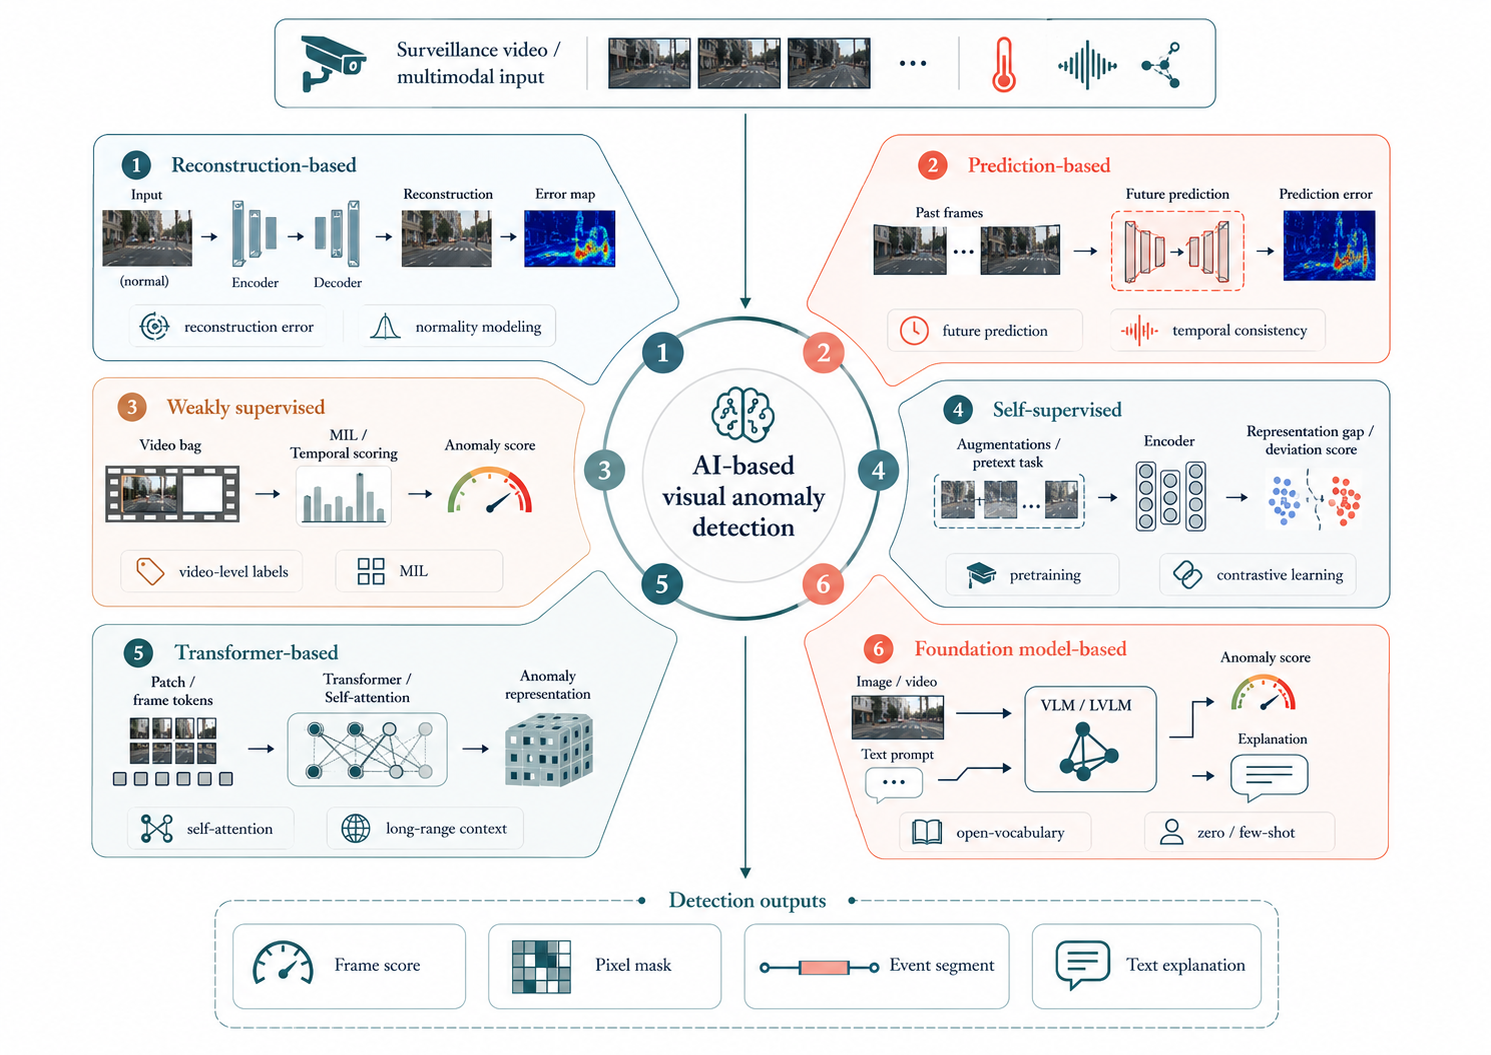
\includegraphics[width=\textwidth]{methods_overview.png}
\caption{Representative method families and their anomaly-evidence signals. Badges distinguish training information, representation, and test-time evidence. The families are navigation lenses rather than mutually exclusive paradigms; a single study can occupy several boxes under the separable coding in Table~\ref{tab:orthogonal_coding}.}
\label{fig:methods_overview}
\end{figure*}


% =============================================
\subsection{Reconstruction-Based Methods}
\label{subsec:reconstruction}

Reconstruction-based methods constitute the foundational paradigm for unsupervised video anomaly detection. The central principle is to train a model exclusively on normal video data such that it learns to faithfully reproduce normal visual patterns; at inference time, anomalous inputs that fall outside the learned normality distribution are expected to produce elevated reconstruction errors.

Formally, given an input frame or frame sequence $\mathbf{x}_t$, a reconstruction model $f_\theta$ produces a reconstructed output $\hat{\mathbf{x}}_t = f_\theta(\mathbf{x}_t)$, and the anomaly score is defined as:
\begin{equation}
    s(\mathbf{x}_t) = \| \mathbf{x}_t - \hat{\mathbf{x}}_t \|_p
    \label{eq:recon_score}
\end{equation}
where $\|\cdot\|_p$ denotes the $\ell_p$-norm (typically $p=2$). A higher reconstruction error indicates a greater likelihood of anomaly.

\subsubsection{Convolutional Autoencoder Approaches}

The earliest deep learning-based reconstruction methods for VAD employed convolutional autoencoders (ConvAEs), in which an encoder $\mathcal{E}_\phi$ compresses input frames into a bottleneck latent representation $\mathbf{z} = \mathcal{E}_\phi(\mathbf{x}_t)$, and a decoder $\mathcal{D}_\psi$ reconstructs the output $\hat{\mathbf{x}}_t = \mathcal{D}_\psi(\mathbf{z})$. Hasan et al.~\citeyearpar{hasan2016learning} were among the first to demonstrate that a ConvAE trained on normal video clips could effectively separate normal from anomalous frames based on reconstruction error magnitude on the UCSD and CUHK Avenue datasets. Subsequent work by Chong and Tay~\citeyearpar{chong2017abnormal} extended this framework to spatiotemporal volumes by processing short video clips as three-dimensional tensors, enabling the model to capture short-range motion dynamics in addition to spatial appearance. Luo et al.~\citeyearpar{luo2017revisit} proposed a stacked-RNN framework that unrolls a sparse-coding objective and imposes a temporal-coherence constraint on successive reconstructions, preventing the autoencoder from generating inconsistent outputs across consecutive frames; the same group separately applied convolutional LSTM to retain longer-range appearance history within the reconstruction pathway~\citep{luo2017remembering}.

A persistent challenge with vanilla autoencoders is their tendency to generalize excessively, reconstructing even anomalous inputs with moderate fidelity when the model capacity is sufficiently large. To address this problem, Gong et al.~\citeyearpar{gong2019memorizing} introduced the Memory-Augmented Autoencoder (MemAE), which interposes a differentiable memory module between the encoder and decoder. Rather than passing the encoded features directly to the decoder, the MemAE retrieves the most similar prototypical normal patterns from a learned memory bank and reconstructs from these prototypes, ensuring that the decoder can only produce outputs that closely resemble memorized normal patterns. Park et al.~\citeyearpar{park2020learning} further refined this concept with the MNAD framework, which combines memory-guided reconstruction with a prediction branch, allowing the model to leverage complementary reconstruction and prediction signals for more robust anomaly scoring.

\subsubsection{Variational and Adversarial Generative Approaches}

Variational autoencoders (VAEs)~\citep{kingma2013auto} augment the reconstruction framework with a probabilistic latent space, enabling density-based anomaly scoring in addition to reconstruction error. Under this formulation, the encoder parameterizes an approximate posterior distribution $q_\phi(\mathbf{z}|\mathbf{x}_t) = \mathcal{N}(\boldsymbol{\mu}_\phi, \boldsymbol{\sigma}_\phi^2)$, and the training objective combines reconstruction fidelity with a Kullback-Leibler divergence regularizer:
\begin{equation}
    \mathcal{L}_{\text{VAE}} = \mathbb{E}_{q_\phi(\mathbf{z}|\mathbf{x})} \left[ -\log p_\psi(\mathbf{x}|\mathbf{z}) \right] + D_{\text{KL}}\left( q_\phi(\mathbf{z}|\mathbf{x}) \| p(\mathbf{z}) \right)
    \label{eq:vae_loss}
\end{equation}
where $p(\mathbf{z})$ is a standard Gaussian prior. At inference, the anomaly score can incorporate both the reconstruction error and the latent-space likelihood, providing a richer signal for anomaly discrimination. Lu et al.~\citeyearpar{lu2020few} employed conditional VAEs for few-shot scene-adaptive anomaly detection, demonstrating that latent-space conditioning on scene identity enables rapid adaptation to novel surveillance environments with minimal data.

Generative adversarial networks offer a complementary route to the same reconstruction principle, in which the adversarial training objective encourages the generator to produce sharper and more realistic reconstructions than those obtained through pixel-wise loss functions alone. Ravanbakhsh et al.~\citeyearpar{ravanbakhsh2017abnormal} employed a conditional GAN to learn the mapping between optical flow fields and video frames, detecting anomalies through discrepancies between the generated and observed appearances. Sabokrou et al.~\citeyearpar{sabokrou2018adversarially} proposed an adversarially learned one-class classifier that uses the discriminator output directly as an anomaly score, bypassing explicit reconstruction error computation.

\subsubsection{Diffusion-Based Reconstruction}

More recently, denoising diffusion probabilistic models (DDPMs)~\citep{ho2020denoising} have been adapted for reconstruction-based anomaly detection. The key insight is that a diffusion model trained to denoise normal data will produce faithful reconstructions when applied to normal inputs but will ``normalize'' anomalous inputs by reconstructing them as their nearest normal counterpart, yielding large discrepancies. Yan et al.~\citeyearpar{yan2023feature} proposed a feature prediction diffusion model (FPDM) that operates in the feature space rather than pixel space, improving computational efficiency while preserving discriminative power. Diffusion-based image anomaly methods such as AnoDDPM~\citep{wyatt2022anoddpm} are relevant as transferable methodological precedents, but they should not be interpreted as surveillance-video benchmarks unless a video-specific adaptation is evaluated.

Table~\ref{tab:reconstruction_methods} summarizes representative reconstruction-based methods with their architectural choices and reported performance.


\begin{table*}[!t]
\centering
\caption{Comparison of representative reconstruction-based methods for video anomaly detection. AUC (\%) is reported at the frame level. A dash (--) indicates that the cited study does not report a result on that benchmark. Values are reported from the cited studies and are not treated as a controlled leaderboard. Rows shared with other tables (e.g., Conv-AE, MemAE, MNAD, FPDM) are repeated for local reading convenience; the canonical consolidated normal-only comparison and its immediate numerical provenance are given in Table~\ref{tab:consolidated_performance} and Supplementary Material~S4.}
\label{tab:reconstruction_methods}
\renewcommand{\arraystretch}{1.25}
\resizebox{\textwidth}{!}{%
\begin{tabular}{llllcccc}
\toprule
\textbf{Method} & \textbf{Year} & \textbf{Architecture} & \textbf{Key Contribution} & \textbf{Ped2} & \textbf{Avenue} & \textbf{SHTech} & \textbf{Paradigm} \\
\midrule
Conv-AE~\citep{hasan2016learning} & 2016 & ConvAE & First end-to-end ConvAE for VAD & 85.0 & 80.0 & 60.9 & Unsupervised \\
Stacked RNN~\citep{luo2017revisit} & 2017 & AE + sparse coding & Temporal coherence regularization & 92.2 & 81.7 & 68.0 & Unsupervised \\
ConvLSTM-AE~\citep{chong2017abnormal} & 2017 & ConvLSTM-AE & Spatiotemporal volume reconstruction & 88.1 & 77.0 & -- & Unsupervised \\
MemAE~\citep{gong2019memorizing} & 2019 & AE + memory & Memory-augmented prototype retrieval & 94.1 & 83.3 & 71.2 & Unsupervised \\
AnoPCN~\citep{ye2019anopcn} & 2019 & AE + prediction & Appearance-motion correspondence & 96.8 & 86.2 & 73.6 & Unsupervised \\
MNAD~\citep{park2020learning} & 2020 & AE + memory + pred. & Memory-guided dual-branch & 97.0 & 88.5 & 70.5 & Unsupervised \\
FPDM~\citep{yan2023feature} & 2023 & Feature Diffusion & Feature-space diffusion prediction & -- & 90.1 & 78.6 & Unsupervised \\
\bottomrule
\end{tabular}%
}
\end{table*}


\textbf{Discussion.} Reconstruction-based methods offer the advantage of requiring no anomalous training data, making them well-suited to practical surveillance deployments where anomalies cannot be enumerated in advance. However, they share a fundamental limitation: the anomaly score depends on the model's inability to reconstruct unfamiliar patterns, which can be unreliable when the model capacity is high or when anomalous patterns share low-level visual statistics with normal ones. The introduction of memory modules, adversarial training, and diffusion-based formulations represents a progressive refinement aimed at sharpening the separation between normal and anomalous reconstruction fidelity.


% =============================================
\subsection{Prediction-Based Methods}
\label{subsec:prediction}

Prediction-based methods reformulate anomaly detection as a temporal forecasting problem: given a sequence of past frames $\{\mathbf{x}_{t-k}, \ldots, \mathbf{x}_{t-1}\}$, the model is trained to predict the next frame $\hat{\mathbf{x}}_t$ or its corresponding optical flow field $\hat{\mathbf{o}}_t$. The underlying assumption is that the temporal dynamics of normal events are sufficiently regular to be predicted accurately, whereas anomalous events introduce unpredictable discontinuities that manifest as large prediction errors:
\begin{equation}
    s(\mathbf{x}_t) = \| \mathbf{x}_t - \hat{\mathbf{x}}_t \|_2^2 + \lambda \| \mathbf{o}_t - \hat{\mathbf{o}}_t \|_2^2
    \label{eq:pred_score}
\end{equation}
where $\lambda$ balances appearance and motion prediction components.

\subsubsection{Frame and Optical-Flow Prediction}

Liu et al.~\citeyearpar{liu2018future} established the dominant baseline for prediction-based VAD by training a U-Net generator within an adversarial framework to predict the next video frame from a short input sequence, incorporating intensity loss, gradient loss, optical flow loss, and adversarial loss to produce sharp and temporally coherent predictions. This work reported higher frame-level AUC than earlier reconstruction-based approaches on the UCSD Ped2, CUHK Avenue, and ShanghaiTech benchmarks under the training regime and evaluation code used in that study; consistent with the comparability procedure of Figure~\ref{fig:comparability_tree}, this should be read as evidence for the prediction paradigm's promise rather than as a controlled head-to-head ranking, since backbone, preprocessing, and post-processing also differ across the compared methods. Subsequent enhancements include the incorporation of attention mechanisms to focus prediction on motion-salient regions~\citep{lee2019bman}, hierarchical graph representations for modeling inter-object relational dynamics~\citep{morais2019learning}, and multi-scale prediction architectures that capture both local and global motion patterns~\citep{chang2022video}.

Beyond appearance, motion itself can serve as the prediction target. Rather than predicting raw RGB frames, several methods operate directly on optical flow representations, which explicitly encode motion information and are more directly related to the behavioral anomalies that are the primary detection target in surveillance. Nguyen and Meunier~\citeyearpar{nguyen2019anomaly} proposed a two-stream architecture that separately predicts appearance and optical flow and fuses their anomaly scores for final detection. Liu et al.~\citeyearpar{liu2021hybrid} introduced a hybrid framework combining memory-augmented flow reconstruction with flow-guided frame prediction, demonstrating that the complementary signals from appearance and motion modalities yield more robust detection across diverse anomaly types.

\subsubsection{Spatiotemporal Prediction with Transformers}

The introduction of transformer architectures to prediction-based VAD has enabled the modeling of long-range temporal dependencies that were difficult to capture with convolutional and recurrent models. Yuan et al.~\citeyearpar{yuan2021transanomaly} proposed TransAnomaly, which replaces the convolutional encoder-decoder with a spatial-temporal transformer network that attends to both local patch features and global frame-level context. Chen et al.~\citeyearpar{chen2022comprehensive} coupled context recovery with a bi-directional predictive network (CR-BPN), using future- and past-frame prediction jointly to capture anomaly-relevant patterns at multiple temporal scales.

Table~\ref{tab:prediction_methods} summarizes representative prediction-based methods.


\begin{table*}[!t]
\centering
\caption{Comparison of representative prediction-based methods for video anomaly detection. AUC (\%) is reported at the frame level.}
\label{tab:prediction_methods}
\renewcommand{\arraystretch}{1.25}
\resizebox{\textwidth}{!}{%
\begin{tabular}{llllcccc}
\toprule
\textbf{Method} & \textbf{Year} & \textbf{Architecture} & \textbf{Key Contribution} & \textbf{Ped2} & \textbf{Avenue} & \textbf{SHTech} & \textbf{Pred. Target} \\
\midrule
Frame-Pred~\citep{liu2018future} & 2018 & U-Net + GAN & Multi-loss future frame prediction & 95.4 & 85.1 & 72.8 & RGB frame \\
Morais et al.~\citeyearpar{morais2019learning} & 2019 & MPED-RNN & Skeleton trajectory prediction & -- & 88.3 & 75.4 & Pose \\
BMAN~\citep{lee2019bman} & 2020 & BiDirectional & Bidirectional multi-scale prediction & 96.6 & 90.0 & 76.2 & RGB frame \\
CT-D2GAN~\citep{feng2021ct} & 2021 & Conv-Transf + D2GAN & Conv-Transformer dual discriminator & 97.2 & 85.9 & 77.7 & RGB frame \\
Hybrid Flow~\citep{liu2021hybrid} & 2021 & MemAE + flow pred. & Memory-augmented flow reconstruction & 96.3 & 85.8 & 73.2 & Flow + RGB \\
CR-BPN~\citep{chen2022comprehensive} & 2022 & Bi-prediction net & Context recovery + bi-directional pred. & 98.3 & 90.3 & 78.1 & RGB frame \\
STENet~\citep{wang2024stenet} & 2024 & Spatiotemporal enhance & Consistency-enhanced spatiotemporal net & 98.1 & 89.7 & 76.8 & RGB frame \\
\bottomrule
\end{tabular}%
}
\end{table*}


\textbf{Discussion.} Prediction-based methods have frequently reported higher benchmark AUC than pure reconstruction approaches by leveraging the temporal structure of video data (a trend rather than a controlled result, given the protocol differences flagged by Figure~\ref{fig:comparability_tree}), and are particularly effective at detecting anomalies that manifest as unexpected motion patterns. However, they tend to produce false alarms in scenarios with inherent visual unpredictability, such as crowded intersections or locations with variable lighting, where even normal events may be difficult to predict precisely. Furthermore, prediction-based methods are most effective for detecting motion-related anomalies and may be less sensitive to static anomalies such as abandoned objects or camera occlusion.


% =============================================
\subsection{Density-, Distance-, and Normalizing-Flow Methods}
\label{subsec:density_flow}
Density- and distance-based methods estimate how probable a test representation is under a model of normality rather than reconstructing the input explicitly. Let $\phi(\mathbf{x}_t)$ be a learned or structured representation and $p_{\theta}$ a density model fitted on normal data. A generic score is
\begin{equation}
  s_{\mathrm{dens}}(\mathbf{x}_t)=-\log p_{\theta}\!\left(\phi(\mathbf{x}_t)\right), \label{eq:density_score}
\end{equation}
with high negative log-likelihood indicating deviation from the learned normal distribution. Nearest-prototype and memory-bank methods use an analogous feature-space distance when an explicit normalized density is unavailable.

Normalizing flows are attractive because they provide tractable likelihoods through invertible transformations, but their performance depends strongly on the representation and on whether likelihood aligns with semantic abnormality. STG-NF~\citep{hirschorn2023normalizing} applies a normalizing flow to spatiotemporal human-pose graphs, yielding a compact, privacy-lean behavioral representation. It is therefore coded as normal-only supervision, density scoring, and graph/pose representation, not as a transformer or self-supervised pretext method. Its strengths on human-pose anomalies do not imply suitability for fire, smoke, or feed corruption, whose discriminative cues are absent from skeletal inputs.

\begin{table*}[!t]
\centering
\caption{Representative density- and distance-based evidence. Values are literature-reported frame-level AUC (\%) where available. Rows shared with other tables (MemAE, MNAD, STG-NF) are repeated for local reading convenience; the canonical consolidated comparison and provenance appear in Table~\ref{tab:consolidated_performance} and Supplementary Material~S4.}
\label{tab:density_methods}
\renewcommand{\arraystretch}{1.22}
\resizebox{\textwidth}{!}{%
\begin{tabular}{p{3.0cm}p{1.3cm}p{3.0cm}p{4.6cm}ccc}
\toprule
\textbf{Method} & \textbf{Year} & \textbf{Representation} & \textbf{Anomaly evidence} & \textbf{Ped2} & \textbf{Avenue} & \textbf{SHTech} \\
\midrule
STG-NF~\citep{hirschorn2023normalizing} & 2023 & Pose graph + normalizing flow & Negative log-likelihood of normal pose dynamics & -- & -- & 85.9 \\
MemAE~\citep{gong2019memorizing} & 2019 & CNN memory prototypes & Distance/reconstruction constrained by normal prototypes & 94.1 & 83.3 & 71.2 \\
MNAD~\citep{park2020learning} & 2020 & Memory-guided appearance/motion & Prototype distance combined with prediction/reconstruction & 97.0 & 88.5 & 70.5 \\
\bottomrule
\end{tabular}%
}
\end{table*}

\textbf{Discussion.} Density-based scores are principled when the representation preserves target-tier cues and the learned density is calibrated. They can nevertheless assign high likelihood to semantically anomalous inputs or low likelihood to benign domain shifts. Cross-scene testing and out-of-distribution calibration are therefore essential.

% =============================================
\subsection{Weakly Supervised and Multiple Instance Learning Methods}
\label{subsec:weakly_supervised}

Weakly supervised methods address the practical reality that frame-level annotations are prohibitively expensive for large-scale surveillance data, while video-level labels indicating the presence or absence of anomalous content are relatively inexpensive to obtain. The dominant formulation employs Multiple Instance Learning (MIL), in which each video is treated as a ``bag'' of frame-level ``instances,'' and the model learns to identify the instances responsible for the bag-level positive label.

Sultani et al.~\citeyearpar{sultani2018real} pioneered this approach with the release of the UCF-Crime dataset and a MIL-based ranking loss that encourages the maximum anomaly score within positive (anomalous) videos to exceed the maximum score within negative (normal) videos:
\begin{equation}
    \mathcal{L}_{\text{MIL}} = \max\left(0, 1 - \max_i s(\mathbf{x}_i^+) + \max_j s(\mathbf{x}_j^-)\right) + \lambda_1 \mathcal{L}_{\text{smooth}} + \lambda_2 \mathcal{L}_{\text{sparse}}
    \label{eq:mil_loss}
\end{equation}
where the smoothness and sparsity constraints regularize the predicted anomaly scores to be temporally coherent and concentrated, respectively.

Tian et al.~\citeyearpar{tian2021weakly} introduced Robust Temporal Feature Magnitude Learning (RTFM), which replaces the simple max-score selection with a top-$k$ feature magnitude learning strategy that mitigates the noise sensitivity of single-instance selection. Feng et al.~\citeyearpar{feng2021mist} proposed the MIST framework, which incorporates multi-instance self-training with pseudo-label refinement, reporting improved frame-level AUC over prior weakly supervised baselines on both UCF-Crime and ShanghaiTech under the study's own protocol. Huang et al.~\citeyearpar{wu2022self} introduced self-guided temporal discriminative transformers that learn temporal context-aware anomaly representations through weakly supervised optimization.

The XD-Violence dataset~\citep{wu2020not} extended the weakly supervised paradigm to multimodal detection by incorporating audio alongside video, motivating methods that fuse visual and acoustic anomaly cues. Chen et al.~\citeyearpar{chen2023mgfn} developed MGFN, a multi-granularity feature network that processes visual features at multiple temporal scales to capture both rapid and prolonged anomalous events. Li et al.~\citeyearpar{li2022self} proposed dual-branch architectures that simultaneously process normal and anomalous feature streams, achieving more stable optimization in the presence of label noise. Table~\ref{tab:weakly_methods} summarizes these methods with their scoring mechanisms and literature-reported results.


\begin{table*}[!t]
\centering
\caption{Comparison of representative weakly supervised methods for video anomaly detection. UCF-Crime and ShanghaiTech use frame-level AUC (\%); XD-Violence uses AP (\%). Values are literature-reported under method-specific protocols. Rows shared with the consolidated comparison are repeated for local reading convenience; the canonical weakly supervised comparison and its provenance appear in Table~\ref{tab:weak_foundation_performance} and Supplementary Material~S4.}
\label{tab:weakly_methods}
\renewcommand{\arraystretch}{1.25}
\resizebox{\textwidth}{!}{%
\begin{tabular}{lllccccc}
\toprule
\textbf{Method} & \textbf{Year} & \textbf{Feature Extractor} & \textbf{UCF-Crime} & \textbf{SHTech} & \textbf{XD-Violence (AP)} & \textbf{Multimodal} & \textbf{Key Innovation} \\
\midrule
MIL-Rank~\citep{sultani2018real} & 2018 & C3D / I3D & 75.4 & -- & -- & No & First MIL framework + UCF-Crime dataset \\
GCN-Anomaly~\citep{zhong2019graph} & 2019 & TSN + GCN & 82.1 & 84.4 & -- & No & Graph-based action-aware features \\
RTFM~\citep{tian2021weakly} & 2021 & I3D & 84.3 & 97.2 & 77.8 & No & Top-$k$ feature magnitude learning \\
MIST~\citep{feng2021mist} & 2021 & I3D & 82.3 & 94.8 & -- & No & Multi-instance self-training \\
Wu et al.~\citeyearpar{wu2020not} & 2020 & I3D + VGGish & 82.4 & -- & 78.6 & Yes & XD-Violence dataset + HL-Net \\
MGFN~\citep{chen2023mgfn} & 2023 & I3D & 86.7 & -- & 80.1 & No & Multi-granularity feature network \\
UR-DMU (RGB)~\citep{zhou2023dmu} & 2023 & I3D & 87.0 & -- & 81.7 & No & Uncertainty-regulated normal/abnormal memories \\
UR-DMU (RGB+audio)~\citep{zhou2023dmu} & 2023 & I3D + VGGish & -- & -- & 81.8 & Yes & Modality ablation using the same UR-DMU model \\
PEL4VAD~\citep{zhang2024pel4vad} & 2024 & I3D + CLIP prompt features & 86.8 & 98.1 & 85.6 & No & Prompt-enhanced context learning \\
\bottomrule
\end{tabular}%
}
\end{table*}


\textbf{Discussion.} Weakly supervised methods achieve a favorable trade-off between annotation cost and detection performance, making them highly practical for large-scale deployment. The MIL framework has proven versatile, accommodating diverse architectural choices from convolutional feature extractors to graph neural networks and transformers. However, the inherent ambiguity of video-level labels means that these methods can misattribute anomaly scores to contextually co-occurring normal events, particularly in videos where anomalous and normal activities are temporally interleaved. UR-DMU is a single 2023 AAAI method rather than separate DMU and UR-DMU publications. Its reported XD-Violence AP changes only from 81.66\% with RGB features to 81.77\% with RGB plus VGGish audio in the paper's modality comparison; this small difference does not support a general claim that audio fusion is uniformly transformative.


% =============================================
\subsection{Self-Supervised and Pretext Task Methods}
\label{subsec:self_supervised}

Self-supervised learning offers an alternative to explicit anomaly labels by training models on automatically generated surrogate tasks that encourage the learning of representations sensitive to the structural regularities of normal video data. At inference, anomalous inputs that violate these learned regularities produce degraded performance on the pretext task, yielding an anomaly signal.

\subsubsection{Pretext-Task and Contrastive Learning Approaches}

Georgescu et al.~\citeyearpar{georgescu2021anomaly} proposed a multi-task self-supervised framework in which the model simultaneously performs arrow-of-time prediction (determining whether a video clip is played forward or backward), motion irregularity estimation, and middle frame reconstruction. The rationale is that normal videos exhibit consistent temporal ordering and motion coherence, while anomalous events disrupt these properties. Wang et al.~\citeyearpar{wang2022video_jigsaw} extended this concept with a video jigsaw puzzle pretext task, in which the model learns to reassemble spatiotemporally shuffled video patches, with anomalous frames producing systematically lower reassembly accuracy due to their violation of learned normal spatiotemporal structure.

A complementary line of work replaces hand-designed pretext objectives with contrastive representation learning, in which methods learn to distinguish between positive pairs (augmentations of the same normal video clip) and negative pairs (clips from different temporal locations or scenes), producing an embedding space in which normal patterns cluster tightly while anomalous patterns occupy distant regions. Formally, given an anchor embedding $\mathbf{z}_i$, its positive counterpart $\mathbf{z}_i^{+}$, and a set of negatives $\{\mathbf{z}_j^{-}\}_{j=1}^{N}$, these methods minimize the InfoNCE objective
\begin{equation}
    \mathcal{L}_{\text{NCE}} = -\log \frac{\exp\!\left(\operatorname{sim}(\mathbf{z}_i, \mathbf{z}_i^{+})/\kappa\right)}{\exp\!\left(\operatorname{sim}(\mathbf{z}_i, \mathbf{z}_i^{+})/\kappa\right) + \sum_{j=1}^{N} \exp\!\left(\operatorname{sim}(\mathbf{z}_i, \mathbf{z}_j^{-})/\kappa\right)}, \label{eq:infonce}
\end{equation}
where $\operatorname{sim}(\cdot,\cdot)$ denotes cosine similarity and $\kappa$ is a temperature parameter; at inference, the anomaly score of a test clip is derived from its distance to the learned normal manifold in the embedding space. Cho et al.~\citeyearpar{cho2023look} proposed a look-around contrastive learning framework that samples temporal neighbors as positive pairs and temporally distant frames as negatives, enabling the model to learn fine-grained temporal consistency features that are disrupted by anomalous events.

\subsubsection{Knowledge Distillation Approaches}

Knowledge distillation-based methods, developed originally for image-level industrial anomaly detection and subsequently imported into the surveillance domain, employ a teacher-student framework in which a pretrained teacher network provides reference representations and a student network is trained to match the teacher's outputs on normal data. At inference, the representation discrepancy between teacher and student serves as an anomaly score,
\begin{equation}
    s_{\text{KD}}(\mathbf{x}_t) = \sum_{\ell \in \mathcal{F}} \left\| f_T^{(\ell)}(\mathbf{x}_t) - f_S^{(\ell)}(\mathbf{x}_t) \right\|_2^2, \label{eq:kd_score}
\end{equation}
where $f_T^{(\ell)}$ and $f_S^{(\ell)}$ denote teacher and student feature maps at layer $\ell$ of a chosen layer set $\mathcal{F}$; the student, trained only on normal data, fails to replicate the teacher's representations for out-of-distribution anomalous inputs, inflating $s_{\text{KD}}$. Salehi et al.~\citeyearpar{salehi2021multiresolution} introduced a multi-resolution knowledge distillation framework that operates at multiple feature scales, improving sensitivity to anomalies of varying spatial extent. Wang et al.~\citeyearpar{wang2021student} further demonstrated that asymmetric teacher-student architectures, in which the student has lower capacity than the teacher, enhance anomaly discrimination by limiting the student's ability to generalize to unseen patterns. Table~\ref{tab:self_supervised_methods} collects the self-supervised and distillation-based evidence, distinguishing the pretext objective from the quantity used as the test-time anomaly score.


\begin{table*}[!t]
\centering
\caption{Comparison of representative self-supervised and knowledge distillation methods for video anomaly detection. AUC (\%) is reported at the frame level. Rows shared with other tables (e.g., Georgescu et al., SSMTL++) are repeated for local reading convenience; the canonical consolidated comparison and provenance appear in Table~\ref{tab:consolidated_performance} and Supplementary Material~S4.}
\label{tab:self_supervised_methods}
\renewcommand{\arraystretch}{1.25}
\resizebox{\textwidth}{!}{%
\begin{tabular}{lllcccc}
\toprule
\textbf{Method} & \textbf{Year} & \textbf{Pretext Task / Mechanism} & \textbf{Ped2} & \textbf{Avenue} & \textbf{SHTech} & \textbf{Key Innovation} \\
\midrule
Georgescu et al.~\citeyearpar{georgescu2021anomaly} & 2021 & Arrow-of-time + motion + middle frame & 97.8 & 89.3 & 82.7 & Multi-task SSL for VAD \\
Jigsaw~\citep{wang2022video_jigsaw} & 2022 & Spatiotemporal jigsaw puzzle & 96.8 & 87.5 & 75.2 & Spatial + temporal shuffling \\
Cho et al.~\citeyearpar{cho2023look} & 2023 & Contrastive temporal neighbors & 97.6 & 89.8 & 79.3 & Look-around contrastive learning \\
SSMTL++v1~\citep{barbalau2023ssmtl} & 2023 & Multi-task pretexts + CvT & -- & 93.7 & 82.9 & Highest Avenue micro-AUC variant reported by the study \\
SSMTL++v2~\citep{barbalau2023ssmtl} & 2023 & Alternative task/backbone configuration & -- & 91.6 & 83.8 & Variant with stronger ShanghaiTech micro-AUC \\
HSC~\citep{sun2023hierarchical} & 2023 & Reconstruction + hierarchical semantic contrast & 98.1 & 93.7 & 83.4 & Scene/object semantic contrast with motion augmentation \\

\bottomrule
\end{tabular}%
}
\end{table*}

The two SSMTL++ rows are retained separately because the original study reports variant-specific trade-offs: combining the best Avenue value from one variant with the best ShanghaiTech value from another would create a non-existent configuration. HSC is listed here because its defining mechanism is normal-only reconstruction plus hierarchical semantic contrast; pretrained parsing components do not make the complete method a transformer-only detector.

% =============================================
\subsection{Vision Transformer-Based Methods}
\label{subsec:vit_methods}

The introduction of transformer architectures to visual anomaly detection has fundamentally expanded the capacity to model long-range spatiotemporal dependencies, addressing a key limitation of purely convolutional and recurrent approaches. The core operation is scaled dot-product self-attention over a sequence of spatiotemporal tokens,
\begin{equation}
    \operatorname{Attn}(\mathbf{Q}, \mathbf{K}, \mathbf{V}) = \operatorname{softmax}\!\left( \frac{\mathbf{Q}\mathbf{K}^{\top}}{\sqrt{d_k}} \right)\mathbf{V}, \label{eq:attention}
\end{equation}
whose $\mathcal{O}(n^2)$ cost in the token count $n$ underlies both the paradigm's global-context advantage and the efficiency concerns discussed in Section~\ref{subsec:open_challenges}. This subsection reviews the principal strategies through which vision transformers have been adapted for anomaly detection in surveillance.

\subsubsection{Spatial Transformers for Frame-Level Detection}

The Vision Transformer (ViT)~\citep{dosovitskiy2020image} processes images by partitioning them into fixed-size patches, projecting each patch into an embedding vector, and applying multi-head self-attention to model global spatial relationships. For anomaly detection, the self-attention mechanism enables the model to capture interactions between distant spatial regions, such as the relationship between a person's pose and their position relative to restricted zones, which are difficult to model with local receptive fields. Several recent works employ ViT-based encoders within reconstruction or prediction frameworks, replacing convolutional backbones with attention-driven feature extractors. The reviewed evidence for ViT-only frame-level detectors in surveillance is, however, thinner than the volume of transformer-titled work suggests: most systems that report competitive results couple attention with a reconstruction, prediction, or MIL objective rather than using a transformer as a standalone anomaly scorer.

\subsubsection{Spatiotemporal Transformers for Video-Level Detection}

Video-oriented transformer architectures extend self-attention across both spatial and temporal dimensions, enabling the joint modeling of appearance and motion dynamics. TimeSformer~\citep{bertasius2021space} introduces divided space-time attention, computing spatial attention within each frame and temporal attention across frames at each spatial position, achieving efficient spatiotemporal modeling without the cubic complexity of full space-time attention. ViViT~\citep{arnab2021vivit} explores multiple factorization strategies for video transformer design, demonstrating that temporal attention over spatial token summaries (the ``factorized encoder'' variant) achieves competitive performance with substantially reduced computational cost. The Video Swin Transformer~\citep{liu2022video} adapts the shifted window mechanism to spatiotemporal volumes, achieving linear complexity with respect to video resolution while maintaining the ability to attend to non-local patterns through window shifting.

In the anomaly detection context, these architectures have been employed as backbone feature extractors for both normal-only and weakly supervised frameworks. Huang et al.~\citeyearpar{huang2022self} proposed a self-supervised attentive framework that combines spatiotemporal transformer features with adversarial training for robust normality modeling. Hierarchical Semantic Contrast (HSC)~\citep{sun2023hierarchical}, by contrast, is treated in Section~\ref{subsec:self_supervised}: its primary contribution is reconstruction plus scene/object semantic contrast using pretrained parsing cues, not a standalone transformer anomaly-scoring paradigm.

\subsubsection{Hybrid CNN-Transformer Architectures}

Recognizing that CNNs provide strong local spatial inductive biases while transformers excel at global context modeling, several hybrid architectures combine both paradigms. These methods typically use a CNN-based early feature extractor followed by transformer layers for global reasoning, or interleave convolutional and attention blocks throughout the network. Feng et al.~\citeyearpar{feng2021ct} proposed the CT-D2GAN, which combines a convolutional encoder for local feature extraction with a transformer-based temporal reasoning module for capturing long-range frame dependencies, achieving notable improvements on ShanghaiTech. Table~\ref{tab:transformer_methods} compares the representative transformer-based systems; consistent with the coding of Table~\ref{tab:orthogonal_coding}, the rows differ in supervision regime as well as in representation, so the reported values are not attributable to the architecture alone.


\begin{table*}[!t]
\centering
\caption{Comparison of representative transformer-based methods for video anomaly detection. AUC (\%) is reported at the frame level.}
\label{tab:transformer_methods}
\renewcommand{\arraystretch}{1.25}
\resizebox{\textwidth}{!}{%
\begin{tabular}{lllccccl}
\toprule
\textbf{Method} & \textbf{Year} & \textbf{Transformer Type} & \textbf{Ped2} & \textbf{Avenue} & \textbf{SHTech} & \textbf{UCF-Crime} & \textbf{Key Innovation} \\
\midrule
CT-D2GAN~\citep{feng2021ct} & 2021 & CNN + Transf. hybrid & 97.2 & 85.9 & 77.7 & -- & Convolutional-Transformer dual GAN \\

TEVAD~\citep{chen2024tevad} & 2023 & Caption-augmented MIL & -- & -- & -- & 84.9 & Text captions fused with visual MIL features \\
SGTTD~\citep{wu2022self} & 2024 & Self-guided temporal Transf. & -- & -- & 97.3 & 85.1 & Self-guided temporal discriminative \\
\bottomrule
\end{tabular}%
}
\end{table*}


\textbf{Discussion.} Transformer-based methods offer clear advantages in modeling global context and long-range temporal dependencies, yielding consistent improvements on challenging multi-scene and multi-actor benchmarks. However, these gains come at the cost of increased computational requirements, particularly for full spatiotemporal attention over high-resolution video, and a greater dependence on large-scale training data to realize the potential of attention-based architectures. The trend toward hybrid CNN-Transformer designs reflects a pragmatic compromise that preserves the local feature extraction strengths of convolutions while benefiting from the global reasoning capabilities of attention. A nascent line of work replaces quadratic self-attention with selective state-space models: VADMamba~\citep{lyu2025vadmamba} combines Mamba-based frame prediction and optical-flow reconstruction to retain long-range temporal modeling at reportedly higher inference speed, suggesting that linear-complexity sequence backbones may become a practical middle ground between convolutional efficiency and transformer expressivity, though this rests on a single study and awaits independent replication.


% =============================================
\subsection{Foundation Model and Vision-Language Methods}
\label{subsec:foundation_models}

Large-scale vision-language and multimodal foundation models introduce a new interface for surveillance anomaly analysis: text-specified categories, prompt-based adaptation, and natural-language description without dense frame-level annotation. These capabilities do not establish universal unseen-anomaly detection and must be evaluated under explicit training, adaptation, calibration, and grounding protocols. This subsection reviews the principal strategies through which vision-language models (VLMs) and large multimodal models (LMMs) have been applied to anomaly detection in surveillance. Figure~\ref{fig:foundation_model_diagram} distinguishes adaptation modes and adds temporal aggregation, calibration, abstention, grounding, and explanation-faithfulness checks before operator use.


\begin{figure*}[!t]
\centering
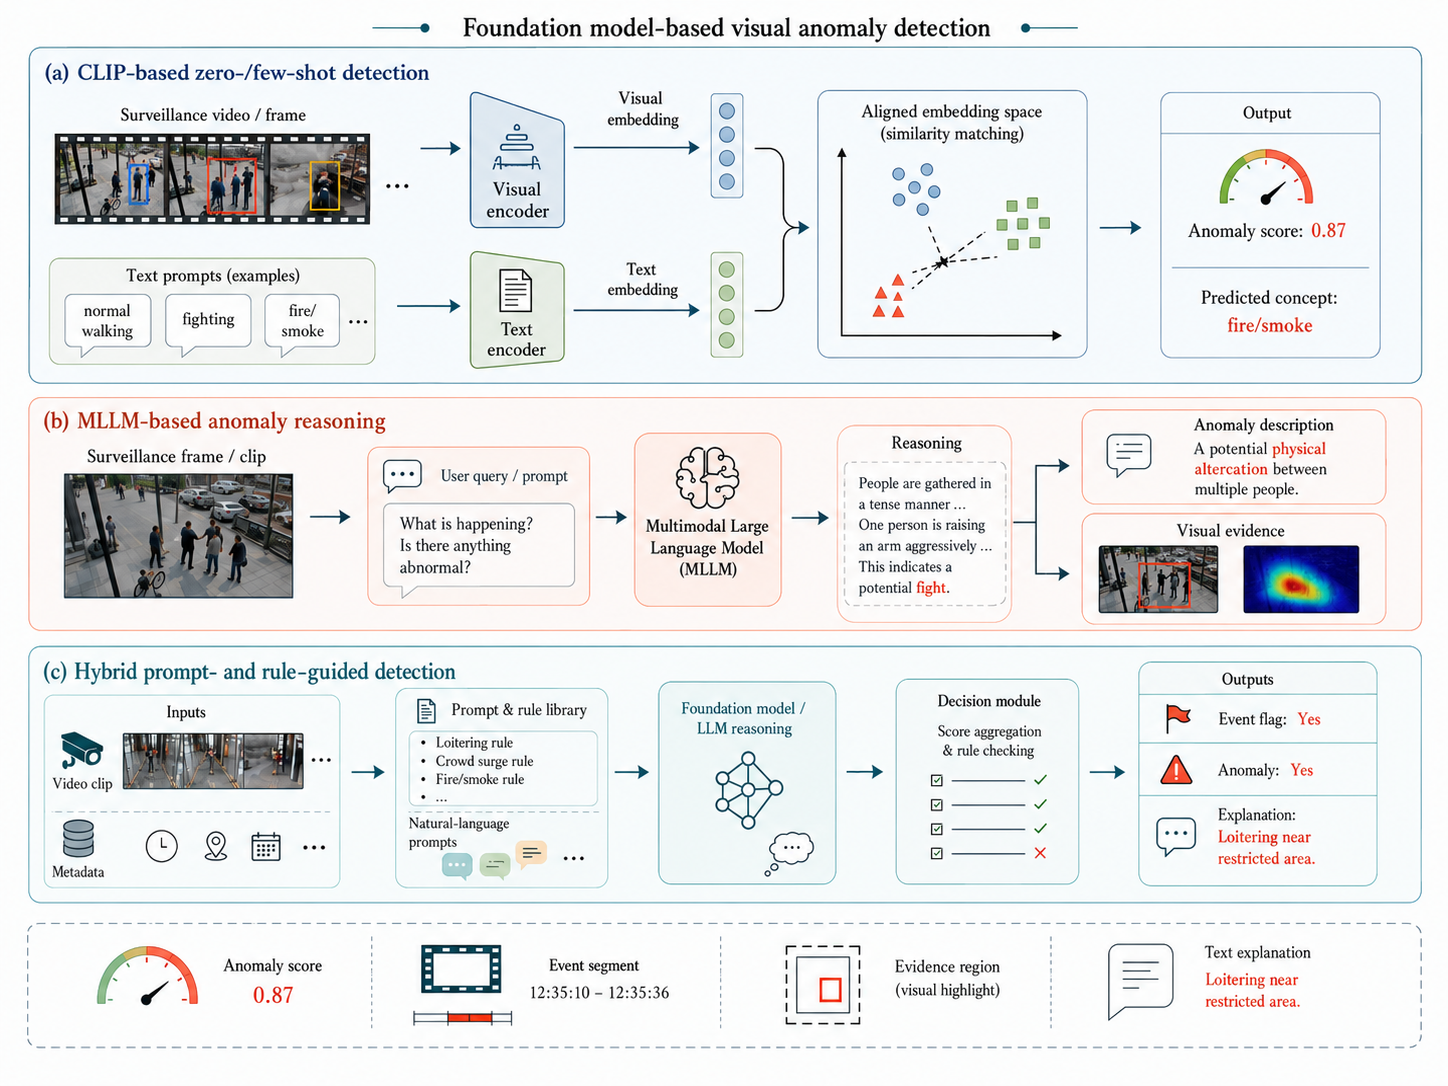
\includegraphics[width=\textwidth]{foundation_model_diagram.png}
\caption{Foundation-model anomaly analysis from adaptation mode to operator-facing output. Training-free prompting, learned prompts/adapters, weakly supervised alignment, and instruction tuning are separated. Temporal aggregation, calibration, abstention, spatial/temporal grounding, and explanation-faithfulness verification are required before natural-language output is treated as decision support.}
\label{fig:foundation_model_diagram}
\end{figure*}

\subsubsection{CLIP-Based Zero-Shot and Few-Shot Detection}

CLIP~\citep{radford2021learning} aligns visual and textual representations in a shared embedding space through contrastive learning on 400 million image-text pairs, enabling zero-shot visual recognition by computing the similarity between image embeddings and textual descriptions of target concepts. For anomaly detection, the approach constructs textual prompts describing normal conditions (e.g., ``a person walking normally on the street'') and anomalous conditions (e.g., ``a person fighting on the street'') and classifies frames based on their relative similarity to these descriptions. Denoting the image encoder by $E_v$ and the text encoder by $E_u$, with prompt sets $\mathcal{P}_{\text{a}}$ (anomalous) and $\mathcal{P}_{\text{n}}$ (normal), we first aggregate each class into a single similarity by max-pooling over its prompts,
\begin{equation}
    S_c(\mathbf{x}_t) = \max_{p \in \mathcal{P}_c} \operatorname{sim}\!\left(E_v(\mathbf{x}_t), E_u(p)\right), \qquad c \in \{\text{a}, \text{n}\}, \label{eq:clip_classscore}
\end{equation}
and the zero-shot frame-level anomaly score is the softmax probability of the anomalous class over the two aggregated scores,
\begin{equation}
    s_{\text{CLIP}}(\mathbf{x}_t) = \frac{\exp\!\left(S_{\text{a}}(\mathbf{x}_t)/\kappa\right)}{\exp\!\left(S_{\text{a}}(\mathbf{x}_t)/\kappa\right) + \exp\!\left(S_{\text{n}}(\mathbf{x}_t)/\kappa\right)}, \label{eq:clip_score}
\end{equation}
which requires no surveillance-specific training; the max-pooling in Equation~\ref{eq:clip_classscore} is one common aggregation choice (mean-pooling and learned prompt weighting are also used), and prompt-learning approaches replace hand-written prompts with learned or structured prompt representations optimized for the target video task.

Wu et al.~\citeyearpar{wu2024vadclip} proposed VadCLIP, a dual-branch framework that combines CLIP-based language--visual alignment with a visual classification branch. Its original coarse-grained evaluation covers UCF-Crime and XD-Violence; ShanghaiTech values should not be attributed to VadCLIP without a separate adaptation source. Zanella et al.~\citeyearpar{zanella2024harnessing} demonstrated that carefully engineered textual prompts can enable CLIP to achieve competitive anomaly detection performance without any training on surveillance-specific data, establishing the viability of fully zero-shot deployment. Subsequent video-specific work has explored structured action-centric prompting and customizable large vision-language model inference, emphasizing that prompt granularity, temporal context, and calibration materially affect zero-shot behavior.

\paragraph{2025--2026 update.} Official WACV/CVPR 2026 proceedings show rapid diversification beyond frozen CLIP scoring. AnyAnomaly~\citep{ahn2026anyanomaly} supports user-defined anomaly concepts through context-aware visual question answering; ASK-HINT~\citep{zou2026askhint} uses action-centric structured prompts; LAVIDA~\citep{dai2026lavida} combines pseudo-anomaly exposure, token compression, and an MLLM without training on real VAD anomalies; LAS-VAD~\citep{wang2026lasvad} introduces anomaly-connected components and intention reasoning; and Alert-CLIP~\citep{zhu2026alertclip} and Fine-VAD~\citep{zhang2026finevad} target region-level alignment and fine-grained anomaly recognition. VADER~\citep{cheng2026vader} adds relation-aware causal context for anomaly understanding, while T-VAU~\citep{gu2026tvau} grounds text-guided reasoning in spatiotemporal anomaly heatmaps. PrismVAU~\citep{erregue2026prismvau} studies lightweight prompt-refined inference, and CADE~\citep{hashimoto2026cade} extends weakly supervised VAD to continual domain change. Few-shot and fine-grained language alignment are further explored by logical-consistency optimization~\citep{zheng2026lco} and REBA~\citep{chu2026reba}. Concurrent weak-supervision work addresses weak-label contamination and bias through TLMA~\citep{xu2026tlma}, denoising/debiasing~\citep{zhao2026denoising}, and mixture-of-memory experts~\citep{sun2026memoryexperts}. Main-conference, findings, and workshop papers are tagged separately in the supplementary evidence table and are not force-ranked because their training information, output granularity, and evaluation protocols differ. A separate arXiv-only empirical assessment reports normal-class bias and recall collapse in zero-shot MLLMs~\citep{yao2026realitycheck}; consistent with our evidence policy, we treat this as an emerging signal rather than as established quantitative evidence, and it is cited only to motivate calibration and event-level testing.

\subsubsection{Large Multimodal Models for Anomaly Reasoning}

Beyond embedding-based similarity, large multimodal models capable of visual question answering and reasoning can generate natural-language descriptions and candidate rationales for detected anomalies, potentially improving operator comprehension when the text is grounded and validated. Tang et al.~\citeyearpar{tang2024hawk} introduced HAWK, a video-language model specifically adapted for open-world video anomaly understanding through instruction tuning on surveillance-relevant visual reasoning tasks. The model can both detect and describe anomalous events in free-form natural language, providing human operators with candidate context beyond a bare anomaly score. Yang et al.~\citeyearpar{yang2024follow} proposed a reasoning-based framework that leverages large language models to follow predefined behavioral rules and flag violations, effectively encoding surveillance policies as natural language specifications.


\begin{table*}[!t]
\centering
\caption{Representative foundation-model and language-guided VAD methods. Training modes and objectives differ; numerical values are retained only where the cited paper reports the same benchmark metric. NR = not reported or not directly comparable. Numerical rows shared with the consolidated comparison are repeated for local reading convenience; canonical values and provenance appear in Table~\ref{tab:weak_foundation_performance} and Supplementary Material~S4.}
\label{tab:foundation_methods}
\renewcommand{\arraystretch}{1.18}
\resizebox{\textwidth}{!}{%
\begin{tabular}{p{3.0cm} c p{3.3cm} p{4.0cm} c c c p{5.1cm}}
\toprule
\textbf{Method} & \textbf{Year} & \textbf{Foundation model} & \textbf{Training/adaptation mode} & \textbf{UCF-Crime} & \textbf{SHTech} & \textbf{XD-Viol. AP} & \textbf{Principal contribution} \\
\midrule
LAVAD~\citep{zanella2024harnessing} & 2024 & CLIP ViT-L/14 & Training-free prompt/video reasoning & 78.1 & -- & -- & Training-free language-guided VAD \\
VadCLIP~\citep{wu2024vadclip} & 2024 & CLIP ViT-B/16 & Video-level weak supervision; frozen CLIP features & 88.0 & -- & 84.5 & Dual-branch visual-language alignment on UCF-Crime/XD-Violence \\
PEL4VAD~\citep{zhang2024pel4vad} & 2024 & I3D + CLIP prompt features & Video-level weak supervision + prompt-enhanced context & 86.8 & 98.1 & 85.6 & Efficient temporal context and anomaly-subclass prompts \\
HAWK~\citep{tang2024hawk} & 2024 & VideoLLaMA & Surveillance instruction tuning & NR & NR & NR & Open-world anomaly understanding and description \\
Follow the Rules~\citep{yang2024follow} & 2024 & LLM/VLM rule pipeline & Rule induction / verification & 80.3 & -- & -- & Explicit normality-rule verification \\
AnyAnomaly~\citep{ahn2026anyanomaly} & 2026 & LVLM & Training-free customizable VQA & NR & NR & NR & User-defined anomaly concepts and cross-dataset testing \\
ASK-HINT~\citep{zou2026askhint} & 2026 & Frozen VLM & Training-free action-centric prompting & NR & NR & NR & Fine-grained prompt groups and guided questions \\
LAVIDA~\citep{dai2026lavida} & 2026 & MLLM & Pseudo-anomaly training; no real VAD training data & NR & NR & NR & Zero-shot frame/pixel detection with token compression \\
Alert-CLIP~\citep{zhu2026alertclip} & 2026 & CLIP & Representation tuning and multi-level alignment & NR & NR & NR & Video-label, region-text, and region-semantic alignment \\
\bottomrule
\end{tabular}%
}
\end{table*}


\textbf{Discussion.} Foundation model-based methods substantially widen the vocabulary of anomalies that can be specified without task-specific annotation. Their generalization beyond that setting is not established by the reviewed evidence, and Section~\ref{subsec:critical_synthesis} sets out why the published validation is narrow. Their ability to operate in zero-shot or few-shot regimes substantially reduces the data requirements for deploying anomaly detection in new environments, and their capacity for natural-language description provides a path toward operator-friendly interfaces, although textual fluency does not by itself establish explanation faithfulness. However, current limitations include computational costs that often hinder real-time edge deployment, CLIP-scale vision-language backbones contain hundreds of millions of parameters and multimodal LLMs several billions, two to four orders of magnitude beyond the lightweight CNNs deployable on surveillance edge hardware, sensitivity to prompt formulation that can significantly affect detection performance, and challenges in achieving fine-grained spatial or temporal localization of anomalies within video streams. The gap between frame-level detection and precise spatiotemporal localization remains a critical open challenge for this paradigm.


% =============================================
\subsection{Structured Temporal Reasoning and Neurosymbolic Methods}
\label{subsec:temporal_neurosymbolic}

The six paradigms reviewed above model time predominantly in an \emph{implicit} manner: 3D convolutions, recurrent units, and attention mechanisms absorb temporal regularities into learned feature representations, and anomalies are flagged when those representations deviate from normality. A smaller but growing body of work instead makes temporal and relational structure \emph{explicit}, through graphs, causal temporal operators, or symbolic rules, and reasons over that structure to reach a detection decision. We review this line as a cross-cutting research direction that spans several method families rather than as a mutually exclusive seventh paradigm.

\textbf{Graph-structured relational modeling.} A first family replaces grid-shaped feature maps with graphs whose nodes are objects, persons, or spatio-temporal regions and whose edges encode interactions. Object-graph formulations learn normal interaction patterns over detected entities and flag anomalous inter-object relations that appearance-based reconstruction would miss; we note that one frequently cited preprint in this line was subsequently withdrawn by its authors for reported inconsistencies, which is itself indicative of how thin the peer-reviewed evidence for this family remains. Skeleton-based methods pursue the same idea for human motion: graph representations of pose sequences underpin both the message-passing formulations discussed in Section~\ref{subsec:self_supervised} and the normalizing-flow model STG-NF~\citep{hirschorn2023normalizing}, whose strong ShanghaiTech results (Table~\ref{tab:consolidated_performance}) demonstrate that compact, structured representations can rival pixel-level models at a fraction of the input dimensionality. In the weakly supervised setting, graph convolutional networks have been used to propagate video-level supervision across temporally correlated segments and to clean noisy labels~\citep{zhong2019graph}.

\textbf{Explicit temporal reasoning.} A second family targets the temporal axis directly. Wu and Liu~\citeyearpar{wu2021causal} introduced a causal temporal relation module that constrains each segment's representation to depend only on current and past observations through causal convolutions, jointly enforcing feature discrimination; the resulting model reaches 84.9\% AUC on UCF-Crime, competitive with contemporaneous feature-magnitude approaches~\citep{tian2021weakly}, while respecting the online, streaming constraint under which deployed surveillance systems must operate. This causal formulation matters operationally: bidirectional temporal context, common in transformer-based methods, is unavailable at inference time in a live feed, so offline benchmark gains do not always translate into deployable improvements. Event-level temporal specifications, for example, that an abandoned-object anomaly is defined by a deposit event followed by a prolonged absence of interaction, exceed what purely statistical temporal models express naturally and motivate the hybrid approaches discussed next.

\textbf{Neurosymbolic and rule-based reasoning.} A third family couples neural perception with symbolic structures. Early work demonstrated that mapping video content onto scene graphs of (subject, predicate, object) triplets supports interpretable anomaly classification, with the symbolic layer exposing \emph{why} a clip was flagged~\citep{chen2018scenegraphs}. MissionGNN~\citep{yun2025missiongnn} scales this idea by generating mission-specific knowledge graphs with a large language model and reasoning over them with a hierarchical graph neural network, achieving weakly supervised anomaly recognition without fine-tuning heavy video encoders. Most recently, rule-induction frameworks use large language models to derive explicit normality rules from a handful of normal reference frames and then verify test frames against those rules~\citep{yang2024follow}, marrying the perceptual breadth of foundation models (Section~\ref{subsec:foundation_models}) with auditable, human-readable decision logic. This family admits a compact formalization: a perception module maps each frame to a symbolic state description $\sigma(\mathbf{x}_t)$ (detected entities, attributes, and relations), a rule set $\mathcal{R} = \{r_1, \ldots, r_m\}$ encodes normality, induced from data, authored by domain experts, or both, and the anomaly score is the weighted degree of rule violation,
\begin{equation}
    s_{\text{NS}}(\mathbf{x}_t) = \sum_{k=1}^{m} w_k \, \mathbb{1}\!\left[ \sigma(\mathbf{x}_t) \nvDash r_k \right], \label{eq:rule_score}
\end{equation}
where $\sigma(\mathbf{x}_t) \nvDash r_k$ denotes that the state fails to satisfy rule $r_k$ and $w_k$ its severity weight. Unlike the learned scoring functions of Equations~\ref{eq:recon_score}--\ref{eq:clip_score}, each nonzero term of Equation~\ref{eq:rule_score} can expose a specific violated rule, making the decision pathway structurally inspectable. This trace is not automatically causally faithful because perception, symbol grounding, rule induction, and weighting can each be wrong. These systems remain early-stage, rule brittleness, symbolic-reasoning latency, and the absence of dedicated benchmarks are unresolved, but they directly address the interpretability and open-set challenges identified in Section~\ref{subsec:open_challenges}, and we examine their future potential in depth in Section~\ref{subsec:future_opportunities}.

Figure~\ref{fig:temporal_validation} replaces qualitative dominance and suitability heatmaps with an explicit mechanism--cue--validation matrix. It records the cue each mechanism is designed to preserve, the principal failure risk, the experiment needed for target-tier validation, and the current evidence status.

\begin{figure*}[!t]
\centering
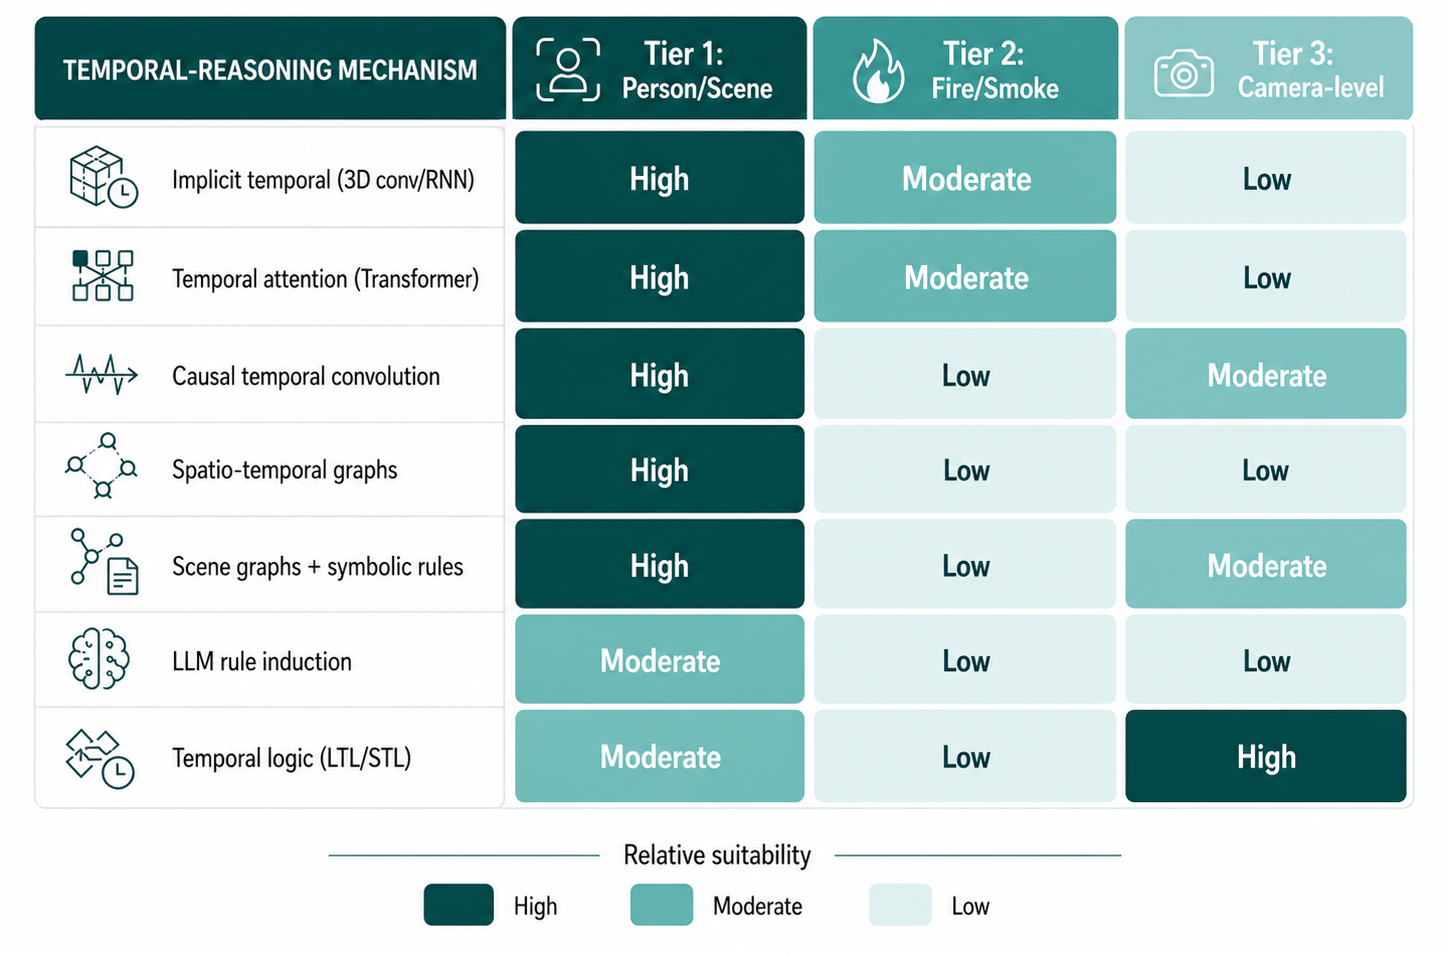
\includegraphics[width=\textwidth]{figure_reasoning_tier_heatmap.png}
\caption{Temporal mechanism--cue compatibility and required validation. The matrix reports design rationale and current evidential status rather than universal high/medium/low suitability scores.}
\label{fig:temporal_validation}
\end{figure*}

% =============================================
\subsection{Fire and Smoke Detection Methods}
\label{subsec:fire_smoke}

Fire and smoke detection through visual sensors has evolved as a specialized subfield that intersects surveillance anomaly detection and environmental hazard monitoring. Unlike behavioral anomalies that are defined by deviations in motion patterns, fire and smoke anomalies are characterized by distinctive photometric properties, including flickering luminance patterns, characteristic color distributions in the yellow-orange-red spectrum for flames and gray-white for smoke, and stochastic boundary dynamics that distinguish them from static scene elements.

\subsubsection{Classification- and Detection-Based Approaches}

Early deep learning methods for fire detection treated the problem as binary image classification, applying pretrained CNNs such as AlexNet, VGGNet, and ResNet as feature extractors with fine-tuned classification heads~\citep{muhammad2019efficient}. These methods achieve high accuracy on constrained datasets but struggle with false positives arising from visually similar phenomena such as sunset reflections, red clothing, and vehicle brake lights. Subsequent work incorporated attention mechanisms and multi-scale feature fusion to improve discrimination between genuine fire regions and confounders~\citep{chen2022fire}.

Moving from whole-image labels to spatial localization, the reformulation of fire and smoke detection as an object detection problem, using architectures such as YOLO~\citep{redmon2016you}, SSD~\citep{liu2016ssd}, and Faster R-CNN~\citep{ren2015faster}, enables both detection and localization of fire regions within the frame. Recent advancements include YOLO-based models optimized for small and distant fire detection in large-scale outdoor settings~\citep{niu2023improved}, deformable convolutional networks that adapt to the irregular and amorphous shapes of smoke plumes~\citep{park2024wildfire}, and transformer-enhanced detectors that leverage global context to disambiguate fire from background clutter~\citep{gao2024twostage}.

\subsubsection{Segmentation-Based Approaches}

Semantic segmentation formulations, based on architectures such as U-Net~\citep{ronneberger2015unet}, DeepLabV3+~\citep{chen2018encoder}, and Mask R-CNN~\citep{he2017mask}, provide pixel-level fire and smoke masks that enable precise boundary delineation and area estimation. These methods are particularly valuable for monitoring fire spread dynamics and assessing damage extent in real time. Guan et al.~\citeyearpar{guan2022improved} developed an improved instance segmentation model based on Mask R-CNN that achieved high precision on the FLAME aerial fire dataset, demonstrating the viability of pixel-level fire segmentation from drone imagery. Because classification accuracy, detection mAP, and segmentation mIoU answer different operational questions and are routinely reported as though they were interchangeable, Table~\ref{tab:fire_methods} sets out the reporting template this review recommends for each task block, together with the early-warning quantities (detection latency, false alarms per monitored hour, confounder performance) that a fire or smoke system intended for deployment must report alongside them.


\begin{table*}[!t]
\centering
\caption{Operational reporting recommended for visual fire/smoke evaluation. Classification, detection, and segmentation results should be reported in separate task blocks.}
\label{tab:fire_methods}
\renewcommand{\arraystretch}{1.25}
\resizebox{\textwidth}{!}{%
\begin{tabular}{p{3.4cm}p{6.8cm}p{8.0cm}}
\toprule
\textbf{Evaluation component} & \textbf{Recommended reporting} & \textbf{Why it matters} \\
\midrule
Task/metric & Classification: balanced accuracy, precision/recall/F1; detection: AP/mAP with IoU threshold; segmentation: IoU/mIoU/Dice & Prevents incomparable metrics from being interpreted as a common leaderboard \\
Phenomenon breakdown & Fire-only, smoke-only, combined; small/early-stage versus developed events & Early smoke and small distant flame are operationally harder than large visible fires \\
False-alarm confounders & Fog, steam, clouds, dust, sunlight, reflections, red/orange objects, emergency lighting & Deployment reliability is dominated by visually similar non-hazard events \\
Temporal performance & Time-to-first-detection, event recall, fragmentation, stability after onset & Frame accuracy can conceal late or intermittent alerts \\
Generalization & Cross-dataset, day/night, weather, indoor/outdoor, RGB/thermal transfer & Custom random splits overestimate operational robustness \\
Efficiency & End-to-end FPS/latency, hardware, input resolution, parameters/FLOPs, power where available & Supports edge-deployment decisions and fair comparison \\
\bottomrule
\end{tabular}%
}
\end{table*}


\textbf{Discussion.} Fire and smoke detection has benefited substantially from the broader advances in object detection and segmentation architectures, with YOLO variants and transformer-based detectors achieving strong performance on increasingly challenging benchmarks. Key remaining challenges include the reliable detection of small and early-stage fires before they become visually prominent, the disambiguation of smoke from fog, dust, and cloud under diverse atmospheric conditions, and the need for real-time processing on resource-constrained edge devices deployed in remote or outdoor settings.


% =============================================
\subsection{Camera Anomaly Detection Methods}
\label{subsec:camera_anomaly}

Camera and video-feed integrity detection addresses the reliability of the complete imaging and transmission pipeline, identifying events such as intentional tampering, accidental obstruction, defocus degradation, and viewpoint displacement that compromise the reliability of the surveillance feed. Unlike scene-level anomaly detection, camera and video-feed integrity detection typically operates on global or region-level image statistics rather than on object-level features.

Operationally, the tier contains four distinct subproblems that should not be collapsed into one accuracy number: (i) abrupt physical tampering, including covering, spraying, or displacement; (ii) gradual optical degradation, including progressive defocus, condensation, and contamination; (iii) electronic sensor corruption, including noise, stuck pixels, exposure instability, and color artifacts; and (iv) network or transport-stream failure, including frozen streams, repeated frames, packet loss, and compression corruption. These subproblems have different onset definitions, recovery conditions, confounders, and acceptable alert delays.

\subsubsection{Feature-Based Change Detection}

Classical approaches to camera tampering detection formulate the problem as change detection over extracted low-level features, with sudden or sustained deviations from baseline statistics triggering a tampering alert. Mantini and Shah~\citeyearpar{mantini2017signal} framed the decision within signal detection theory, monitoring temporal variations in features such as color histograms, edge density, local binary patterns, and spatial frequency content; the same authors subsequently released UHCTD~\citep{mantini2019uhctd}, described by its authors as the first large-scale public tampering benchmark, and systematically evaluated ten feature types through time series analysis, finding that combinations of edge-based and texture-based features provide the most robust tampering detection across diverse surveillance scenarios.

\subsubsection{Deep Learning Approaches}

Learned representations for camera-anomaly categories remain sparsely reported in the peer-reviewed literature, which is itself one of this review's findings rather than an omission of coverage. The application of autoencoders trained on normal camera feeds for detecting sensor degradation has shown promise, with reconstruction error magnitude providing a continuous indicator of feed quality that can be monitored alongside scene-level anomaly detection.

An emerging approach applies image quality assessment (IQA) models to surveillance feeds as a proxy for camera health monitoring. No-reference IQA methods such as BRISQUE~\citep{mittal2012brisque} and NIQE~\citep{mittal2013niqe}, which evaluate image quality without access to a pristine reference, can detect blur, noise, compression artifacts, and exposure anomalies in real time. When integrated with temporal consistency analysis, these methods provide a lightweight and architecture-agnostic mechanism for continuous camera health surveillance.


% NOTE(editorial revision): the former Table "Comparison of representative methods for camera anomaly and tampering detection" duplicated Table~\ref{tab:sota_camera} and has been merged into it (see Section~\ref{subsec:sota_camera}).


Representative methods for this tier are consolidated in Table~\ref{tab:sota_camera}.

\textbf{Discussion.} Camera and video-feed integrity detection remains a comparatively underdeveloped area that has yet to fully benefit from the deep learning revolution that has transformed scene-level anomaly detection. The majority of existing methods rely on handcrafted features and threshold-based decision rules, offering low computational cost but limited adaptability across cameras, seasons, and fault severities. Future evaluations should separate real from synthetic faults, abrupt from gradual onset, and detection from recovery; they should report fault-severity curves, unseen-camera testing, day/night and seasonal transfer, false alarms per camera-day, time-to-detection, and end-to-end edge throughput. The integration of learned features, temporal modeling, and modular architectures that monitor feed integrity alongside scene content remains promising but insufficiently validated.


% =============================================
\subsection{Summary and Cross-Paradigm Analysis}
\label{subsec:method_summary}

Despite their architectural diversity, all reviewed paradigms instantiate a single mathematical template: each learns (or inherits) a representation map $\phi$, a normality model $\widehat{\mathcal{N}}$, and a discrepancy functional $D$, and scores a test input as
\begin{equation}
    s(\mathbf{x}_t) = D\!\left( \phi(\mathbf{x}_t), \, \widehat{\mathcal{N}} \right).
    \label{eq:unified_score}
\end{equation}
Reconstruction methods take $\phi$ as an encoder-decoder, $\widehat{\mathcal{N}}$ as the manifold of reconstructible patterns, and $D$ as reconstruction error (Equation~\ref{eq:recon_score}); prediction methods replace $D$ with prediction fidelity (Equation~\ref{eq:pred_score}); weakly supervised MIL learns $D$ discriminatively under video-level constraints (Equation~\ref{eq:mil_loss}); self-supervised methods shape $\phi$ so that distance in embedding space realizes $D$ (Equations~\ref{eq:infonce}--\ref{eq:kd_score}); foundation models import a pretrained $\phi$ and express $\widehat{\mathcal{N}}$ in natural language (Equation~\ref{eq:clip_score}); and neurosymbolic methods make $\widehat{\mathcal{N}}$ an explicit rule set (Equation~\ref{eq:rule_score}). Under this template, cross-tier transfer (Section~\ref{subsec:cross_category}) amounts to asking which of the three components, $\phi$, $\widehat{\mathcal{N}}$, or $D$, survives a change of anomaly tier, and which must be re-learned. Table~\ref{tab:cross_paradigm} summarizes the strongest established evidence, principal failure modes, and reporting conditions for each method family.


\begin{table*}[!t]
\centering
\caption{Protocol-aware cross-paradigm synthesis. The table reports established evidence and deployment conditions rather than assigning universal suitability or interpretability grades.}
\label{tab:cross_paradigm}
\renewcommand{\arraystretch}{1.25}
\resizebox{\textwidth}{!}{%
\begin{tabular}{p{3.4cm}p{4.8cm}p{5.4cm}p{5.2cm}}
\toprule
\textbf{Method family} & \textbf{Strongest established evidence} & \textbf{Primary failure mode} & \textbf{Deployment/explanation condition} \\
\midrule
Reconstruction and prediction & Normal-only behavioral VAD on fixed-camera benchmarks & Generalizes enough to reconstruct/predict some anomalies; sensitive to scene unpredictability & Can be efficient; score is not inherently human-interpretable \\
Weakly supervised MIL & Large untrimmed behavioral datasets with video-level labels & Label ambiguity, context leakage, low-recall operating points & Efficient with frozen features; temporal evidence must be localized and calibrated \\
Self-supervised and distillation & Label-free representation learning on normal video & Pretext-task mismatch and scene-specific shortcuts & Useful when anomaly labels are absent; explanation usually requires additional evidence modules \\
Transformers and state-space models & Long-range temporal modeling and multi-scene representations & Data/computation demands; bidirectional context may violate online constraints & Report causal versus offline inference and end-to-end latency \\
Vision-language and MLLM & Open-vocabulary behavior concepts and natural-language descriptions & Prompt sensitivity, weak localization, calibration, hallucinated or unfaithful rationale & Distinguish training-free from adapted models; verify evidence grounding and explanation faithfulness \\
Fire and smoke detectors & Task-specific classification, object detection, and segmentation & Confounders, early low-contrast smoke, domain shift & Report task-specific metrics and time-to-detection \\
Camera/feed-integrity methods & Abrupt tampering and selected quality faults & Camera-specific drift, gradual degradation, proprietary corpora & Report cross-camera validation, false alarms per camera hour, and detection delay \\
\bottomrule
\end{tabular}%
}
\end{table*}


Several cross-cutting observations emerge from this analysis. First, no single methodological paradigm achieves strong suitability across all anomaly categories, deployment constraints, and evaluation criteria simultaneously. Reconstruction- and prediction-based methods excel in label-free settings and offer real-time performance but are limited in their capacity to detect novel anomalies that share visual statistics with normal events. Weakly supervised methods achieve competitive accuracy with moderate annotation cost but require at least video-level labels and are primarily validated on person-related anomalies. Foundation-model approaches provide flexible semantic transfer and human-readable descriptions, but published evidence does not establish universal generalization or faithful explanation; computational cost and prompt/calibration sensitivity also constrain deployment. Domain-specific methods for fire detection and camera and video-feed integrity detection achieve specialized performance within their respective domains but are disconnected from broader anomaly detection frameworks.

Second, the trend toward unified architectures that can simultaneously address multiple anomaly categories is accelerating but remains nascent. The practical surveillance system of the future will likely require a compositional approach that integrates complementary detection paradigms, with lightweight domain-specific modules for real-time camera health monitoring and environmental hazard detection operating alongside more computationally intensive scene-level anomaly analysis informed by foundation model reasoning.

Third, the transition from method development to deployment readiness remains a significant gap across all paradigms. Most reported results are obtained under controlled benchmark conditions with standardized evaluation protocols, and the challenges of domain shift, concept drift, privacy constraints, and adversarial robustness that characterize real-world deployment are inadequately addressed by the current literature. We return to these deployment challenges in Section~\ref{sec:discussion}.


\section{Datasets, Benchmarks, and Evaluation}
\label{sec:datasets}

A rigorous evaluation of visual anomaly detection methods requires both well-curated benchmark datasets that capture the diversity of real-world surveillance scenarios and standardized evaluation metrics that enable meaningful cross-method comparison. This section provides a comprehensive survey of the principal evaluation metrics employed across different detection tasks (Section~\ref{subsec:eval_metrics}) and the benchmark datasets that have driven methodological progress in each anomaly category (Section~\ref{subsec:benchmark_datasets}). We conclude with a consolidated performance comparison that synthesizes results across paradigms and datasets (Section~\ref{subsec:performance_analysis}).


% =============================================
\subsection{Evaluation Metrics}
\label{subsec:metrics}
\label{subsec:eval_metrics}

The choice of evaluation metric is dictated by the detection task formulation, particularly by the granularity of the desired output (frame-level versus pixel-level) and the nature of the anomaly category under consideration. Table~\ref{tab:metrics} provides an overview of the principal metrics used across different evaluation scenarios.


\begin{table*}[!t]
\centering
\caption{Evaluation metrics used across surveillance anomaly tasks. Metric names are kept distinct from task names; protocol details such as aggregation, thresholds, and matching rules must be reported.}
\label{tab:metrics}
\renewcommand{\arraystretch}{1.2}
\resizebox{\textwidth}{!}{%
\begin{tabular}{p{2.8cm}p{3.5cm}p{8.0cm}p{4.4cm}}
\toprule
\textbf{Granularity} & \textbf{Metric} & \textbf{Interpretation / required detail} & \textbf{Typical use} \\
\midrule
Frame ranking & ROC-AUC / micro-AUC & Threshold-independent ranking; state whether frames are pooled globally or averaged by video & Ped2, Avenue, ShanghaiTech, UCF-Crime \\
Frame ranking & PR-AUC / AP & Precision-recall ranking under class imbalance; state interpolation/aggregation & XD-Violence and imbalanced WSVAD \\
Operational frame detection & Recall/precision at fixed low FPR; false alarms per hour & Evaluates meaningful operating points rather than global ranking alone & Deployment-oriented VAD \\
Event level & Event precision/recall/F1 at temporal IoU thresholds & Match predicted and ground-truth temporal events using stated tIoU thresholds; report fragmentation and delay & Event-centric VAD~\citep{rashvand2026frames} \\
Pixel level & Pixel-AUC & ROC-AUC over pixels; avoid the ambiguous abbreviation pAUC, which often means partial AUC & Pixel anomaly localization \\
Region level & PRO & Per-region overlap evaluated across a controlled false-positive-rate range & Region-sensitive localization \\
Segmentation & IoU / mIoU / Dice & Spatial overlap of masks; report class averaging and thresholding & Fire and smoke masks and pixel VAD \\
Object detection & AP / mAP & Report IoU threshold(s), class averaging, and confidence calibration & Fire and smoke boxes \\
Camera/feed integrity & F1/EER, detection delay, false alarms per camera hour & Event definition and onset must be explicit; separate abrupt and gradual faults & Tampering, freeze, blur, displacement \\
\bottomrule
\end{tabular}%
}
\end{table*}


\subsubsection{Frame-Level Detection Metrics}
\label{subsubsec:frame_metrics}

The most widely adopted evaluation metric for video anomaly detection is the frame-level Area Under the Receiver Operating Characteristic Curve (AUC-ROC). Given a set of test frames with corresponding ground-truth labels $y_t \in \{0, 1\}$ and predicted anomaly scores $s(\mathbf{x}_t)$, the ROC curve plots the true positive rate (TPR) against the false positive rate (FPR) as the decision threshold $\tau$ varies:
\begin{equation}
    \text{TPR}(\tau) = \frac{|\{t : s(\mathbf{x}_t) > \tau \wedge y_t = 1\}|}{|\{t : y_t = 1\}|}, \quad
    \text{FPR}(\tau) = \frac{|\{t : s(\mathbf{x}_t) > \tau \wedge y_t = 0\}|}{|\{t : y_t = 0\}|}
    \label{eq:tpr_fpr}
\end{equation}
The AUC-ROC provides a threshold-independent assessment of discriminative power, with a value of 1.0 indicating perfect separation and 0.5 indicating random performance. The standard evaluation protocol for the majority of VAD benchmarks, including UCSD Ped2, CUHK Avenue, and ShanghaiTech, computes the \textit{micro-AUC}, which pools all test frames across all test videos before computing the curve, rather than averaging per-video AUCs.

For datasets with severe class imbalance, where normal frames vastly outnumber anomalous ones, the AUC-ROC can be overly optimistic because a high FPR may correspond to a large absolute number of false alarms. In such cases, the Average Precision (AP), computed as the area under the Precision-Recall curve, provides a more informative evaluation. The AP metric has been adopted as the standard for the XD-Violence dataset~\citep{wu2020not} and is increasingly used alongside AUC-ROC for comprehensive evaluation.

Frame-level micro-AUC, despite its ubiquity, has well-documented shortcomings as a headline metric. Because it pools all test frames, long normal segments dominate the score, temporal smoothing of the anomaly signal can raise AUC without improving event detection, and the metric neither rewards spatial localization nor penalizes fragmented detections of a single event. These concerns motivated the region- and track-based criteria (RBDR/TBDR) introduced with the Street Scene benchmark~\citep{ramachandra2020street}, which score detections at the level of anomalous regions and tracks rather than frames. We therefore report AUC values throughout this survey as the field's \emph{de facto} common currency while cautioning that cross-method AUC differences of a few points, particularly on saturated single-scene benchmarks, should not be over-interpreted.

The Equal Error Rate (EER), defined as the error rate at the threshold where the false positive rate equals the false negative rate, is employed primarily in camera tampering detection, where the operational objective is to minimize both missed tampering events and false alarms simultaneously.

\paragraph{Event-centric evaluation.} Frame ranking does not measure whether a coherent anomalous episode is localized with a useful onset, duration, and alert delay. Rashvand et al.~\citeyearpar{rashvand2026frames} adapt temporal-action-localization matching to VAD and report a pronounced gap between frame AUC and event-level precision/F1. Acharya et al.~\citeyearpar{acharya2026road} similarly show that high AUROC can coexist with poor recall at operationally meaningful false-positive rates. Future evaluation should therefore report event precision/recall/F1 across temporal IoU thresholds, detection delay, fragmentation, and recall at fixed low-FPR operating points in addition to frame-level AUC.

\subsubsection{Pixel-Level Localization Metrics}
\label{subsubsec:pixel_metrics}

When pixel-level anomaly localization is required, the evaluation extends to spatial masks. Pixel-level AUC computes the ROC curve over individual pixels, treating each pixel location as an independent binary classification decision. The Intersection over Union (IoU) between predicted and ground-truth anomaly masks provides a region-level evaluation that penalizes both missed anomalous regions and false alarm regions:
\begin{equation}
    \text{IoU} = \frac{|\mathbf{M}_{\text{pred}} \cap \mathbf{M}_{\text{gt}}|}{|\mathbf{M}_{\text{pred}} \cup \mathbf{M}_{\text{gt}}|}
    \label{eq:iou}
\end{equation}
The mean IoU (mIoU), averaged across all anomaly categories and test images, is the standard metric for fire and smoke segmentation tasks. The Per-Region Overlap (PRO) metric, originally popularized in industrial anomaly detection~\citep{bergmann2019mvtec}, averages per-region overlap while controlling the false-positive rate. Its integration range and normalization must be reported; it should not be described simply as connected-component IoU.

\subsubsection{Tier-Specific Metrics: Fire/Smoke and Camera / Feed Integrity Detection}
\label{subsubsec:detection_metrics}

When fire and smoke detection is formulated as an object detection problem, the standard COCO-style metrics~\citep{lin2014microsoft} are employed. The mean Average Precision (mAP) is computed at IoU thresholds of 0.5 (mAP@0.5) and across multiple thresholds from 0.5 to 0.95 (mAP@[0.5:0.95]). The F1-score, computed as the harmonic mean of precision and recall at the optimal confidence threshold, provides a single-number summary of detection performance and is particularly useful for comparing methods with different precision-recall trade-off characteristics.

For the camera/feed-integrity tier, evaluation conventions differ again. Camera and video-feed integrity detection methods are typically evaluated using classification accuracy, F1-score, and detection latency (the time delay between the onset of a camera anomaly and its detection). The false alarm rate (FAR) is given particular emphasis in this domain, as excessive false alarms undermine operator trust and render the monitoring system unreliable in practice. Detection latency is measured in frames or seconds and reflects the practical requirement for timely notification of camera compromise.


% =============================================
\begin{figure*}[!t]
\centering
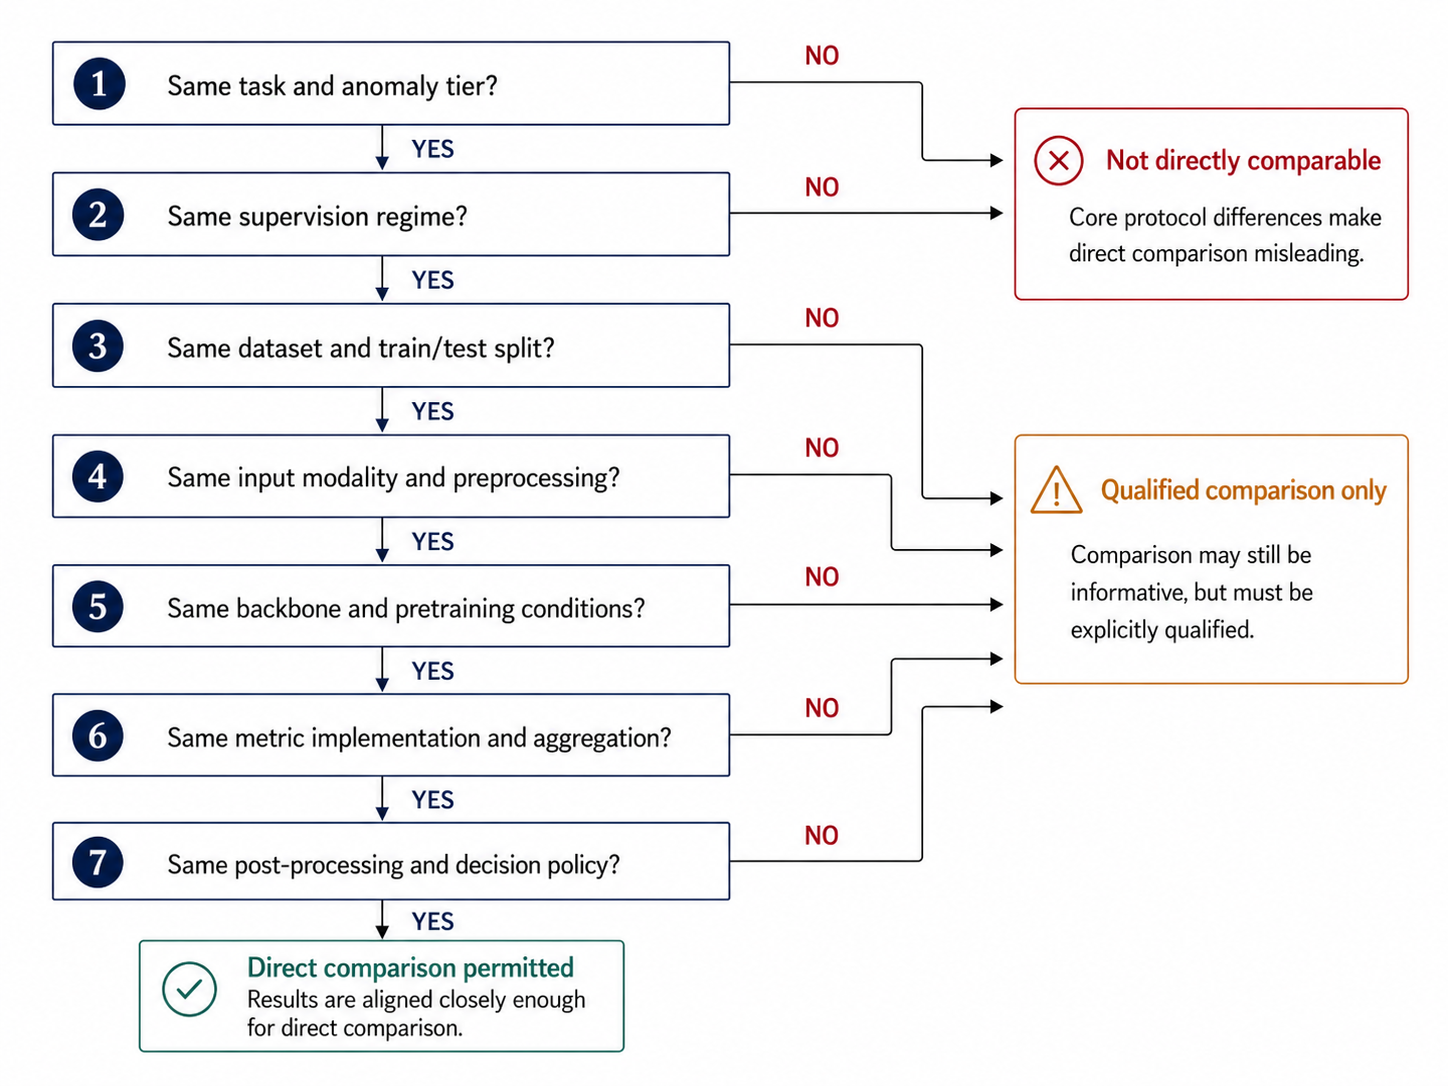
\includegraphics[width=0.88\textwidth]{Protocol Comparability Decision Tree.png}
\caption{Decision tree for deciding whether literature-reported performance values support direct comparison. A single mismatch in task, supervision, split, modality, pretraining, metric implementation, or post-processing requires a qualified comparison rather than a global leaderboard claim.}
\label{fig:comparability_tree}
\end{figure*}

\subsection{Benchmark Datasets}
\label{subsec:benchmark_datasets}

The availability of diverse and well-annotated benchmark datasets has been instrumental in driving methodological progress in visual anomaly detection. This subsection surveys the principal datasets organized by anomaly category, with detailed characteristics summarized in Tables~\ref{tab:vad_datasets},~\ref{tab:fire_datasets}, and~\ref{tab:camera_datasets}.


\subsubsection{Video Anomaly Detection Datasets (Person and Scene)}
\label{subsubsec:vad_datasets}

The landscape of VAD benchmarks has evolved substantially over the past decade, progressing from small-scale, single-scene datasets to large-scale, multi-scene collections with diverse anomaly categories.

\textbf{UCSD Pedestrian (Ped1 and Ped2)}~\citep{mahadevan2010anomaly} is among the earliest and most widely used VAD benchmarks. The dataset captures a single pedestrian walkway, with anomalies defined as the presence of non-pedestrian entities (bicycles, skateboarders, vehicles) or unusual pedestrian motion patterns. Ped1 contains 34 training and 36 testing clips at $158 \times 238$ resolution, while Ped2 contains 16 training and 12 testing clips at $240 \times 360$ resolution. Despite its widespread adoption, the limited scene diversity and narrow anomaly definition have led many recent methods to achieve near-saturated performance (AUC $>$ 97\%), diminishing its discriminative value for evaluating state-of-the-art methods.

\textbf{CUHK Avenue}~\citep{lu2013abnormal} expands scene complexity with 16 training and 21 testing videos captured from a campus avenue, containing 47 anomalous events including running, throwing objects, loitering, and walking in unusual directions. The variable pedestrian density and perspective-dependent size changes make this dataset more challenging than UCSD, and it remains widely used for evaluating unsupervised and self-supervised methods.

\textbf{ShanghaiTech Campus}~\citep{luo2017revisit} represents a significant scaling in both scene diversity and anomaly complexity, comprising 330 training and 107 testing videos captured from 13 different camera locations across a university campus. The dataset contains 130 anomalous \emph{events} drawn from 11 anomaly categories (Table~\ref{tab:vad_datasets}), including chasing, brawling, and cycling in pedestrian zones; the event count and the category count are distinct quantities and should not be conflated. The multi-scene design enables evaluation of cross-scene generalization, a property that is critical for practical deployment.

\textbf{UCF-Crime}~\citep{sultani2018real} introduced the first large-scale, weakly supervised VAD benchmark, containing 1,900 untrimmed surveillance videos with 13 real-world anomaly categories including abuse, arrest, arson, assault, burglary, explosion, fighting, road accidents, robbery, shooting, shoplifting, stealing, and vandalism. The standard split comprises 1,610 training videos (800 normal and 810 anomalous) and 290 test videos. Only video-level labels are provided for training, making this dataset the standard benchmark for MIL-based weakly supervised methods. The large intra-class variability and diverse camera viewpoints make UCF-Crime substantially more challenging than controlled-scene datasets; at the same time, its video-level tags and loose temporal boundaries introduce non-trivial label noise, a limitation repeatedly acknowledged and explicitly targeted by subsequent weakly supervised work~\citep{zhong2019graph, tian2021weakly}.

\textbf{XD-Violence}~\citep{wu2020not} extends the weakly supervised paradigm to multimodal detection, providing both video and audio tracks for 4,754 untrimmed videos spanning six violence categories. The inclusion of audio enables the evaluation of audiovisual fusion strategies and has motivated research into multimodal anomaly detection.

\textbf{UBnormal}~\citep{acsintoae2022ubnormal} represents a distinctive approach to benchmark construction by generating virtual surveillance scenes with synthetically rendered anomalies, providing pixel-level anomaly annotations that are impractical to obtain for real-world video. The dataset contains 29 scenes with both normal and anomalous events rendered using virtual actors, enabling rigorous evaluation of pixel-level localization accuracy.

\textbf{CHAD (Charlotte Anomaly Dataset)}~\citep{pazho2023chad} provides a recent high-resolution benchmark captured from multiple viewpoints, with detailed annotations for diverse behavioral anomalies and normal activities, addressing limitations of older datasets in terms of resolution and annotation granularity.


\begin{table*}[!t]
\centering
\caption{Summary of benchmark datasets for video anomaly detection (person and scene anomalies). Train/Test = number of training/testing videos; Ann. = Annotation level; Cat. = Number of anomaly categories.}
\label{tab:vad_datasets}
\renewcommand{\arraystretch}{1.3}
\resizebox{\textwidth}{!}{%
\begin{tabular}{llccccccl}
\toprule
\textbf{Dataset / corpus} & \textbf{Year} & \textbf{Train} & \textbf{Test} & \textbf{Scenes} & \textbf{Cat.} & \textbf{Ann.} & \textbf{Resolution} & \textbf{Primary Anomaly Types} \\
\midrule
UCSD Ped1~\citep{mahadevan2010anomaly} & 2010 & 34 & 36 & 1 & 3 & Frame + pixel & $158 \times 238$ & Non-pedestrian entities (bikes, carts) \\
UCSD Ped2~\citep{mahadevan2010anomaly} & 2010 & 16 & 12 & 1 & 3 & Frame + pixel & $240 \times 360$ & Non-pedestrian entities (bikes, skaters) \\
UMN~\citep{mehran2009abnormal} & 2009 & -- & 11 & 3 & 1 & Frame & $320 \times 240$ & Crowd panic and escape \\
CUHK Avenue~\citep{lu2013abnormal} & 2013 & 16 & 21 & 1 & 5 & Frame + pixel & $360 \times 640$ & Running, throwing, loitering \\
ShanghaiTech~\citep{luo2017revisit} & 2017 & 330 & 107 & 13 & 11 & Frame & Various & Chasing, brawling, cycling \\
UCF-Crime~\citep{sultani2018real} & 2018 & 1,610 & 290 & Many & 13 & Video-level & Various & 13 real-world crime categories \\
Street Scene~\citep{ramachandra2020street} & 2020 & 46 & 35 & 1 & 17 & Frame + bbox & $1280 \times 720$ & Jaywalking, loitering, vehicle anomalies \\
XD-Violence~\citep{wu2020not} & 2020 & 3,954 & 800 & Many & 6 & Video-level & Various & Violence with audio track \\
ADOC~\citep{doshi2022adoc} & 2020 & -- & 18 & 1 & 5 & Frame & VGA & Campus anomalies + camera tampering \\
UBnormal~\citep{acsintoae2022ubnormal} & 2022 & 268 & 211 & 29 & 22 & Frame + pixel & $720 \times 1080$ & Synthetic scenes with pixel masks \\
NWPU Campus~\citep{cao2023nwpu} & 2023 & 305 & 148 & 43 & 28 & Frame + bbox & $1080$p & Large-scale campus multi-scene \\
CHAD~\citep{pazho2023chad} & 2023 & -- & -- & 4 & 6 & Frame + bbox & HD & High-resolution multi-view \\
\bottomrule
\end{tabular}%
}
\end{table*}


\subsubsection{Fire and Smoke Detection Datasets}
\label{subsubsec:fire_datasets}

Fire and smoke detection benchmarks have evolved from small-scale image classification collections to large-scale multi-source datasets incorporating diverse fire scenarios, imaging modalities, and environmental conditions.

\textbf{FLAME}~\citep{shamsoshoara2021aerial} provides an aerial fire detection benchmark comprising over 2,000 images and 39 video sequences captured by unmanned aerial vehicles during prescribed burns in Northern Arizona. The dataset includes frame-level binary labels and instance segmentation annotations for fire and smoke regions, making it suitable for evaluating both classification and segmentation approaches.

\textbf{FireNet}~\citep{jadon2019firenet} offers a binary classification benchmark with approximately 2,500 images evenly divided between fire and non-fire categories, sampled from diverse indoor and outdoor scenarios. While limited in scale, FireNet has been widely adopted for evaluating lightweight fire classification models intended for edge deployment.

\textbf{FASDD (Flame And Smoke Detection Dataset)}~\citep{wang2024fasdd} represents a recent large-scale contribution, containing over 120,000 heterogeneous images covering various fire types, smoke densities, and environmental conditions. The dataset includes bounding box annotations for both flame and smoke objects and is designed to improve model generalization through data heterogeneity.

\textbf{D-Fire}~\citep{de2022dfire} provides 21,527 images with bounding box annotations for fire and smoke detection in diverse settings, including indoor environments, forests, and urban scenes. The dataset addresses the common limitation of fire detection benchmarks that focus on a single environmental context.

\textbf{FiSmo}~\citep{cazzolato2017fismo} is a compilation of six sub-collections assembled from emergency-situation imagery, including Flickr-Fire (2{,}000 images), BoWFire (226 images), SmokeBlock (1{,}666 images), and annotated video subsets; the sub-collections are reported separately in the source and should not be quoted as a single aggregate.


\begin{table*}[!t]
\centering
\caption{Summary of benchmark datasets for fire and smoke detection. Type: Cls = Classification, Det = Object Detection, Seg = Segmentation.}
\label{tab:fire_datasets}
\renewcommand{\arraystretch}{1.3}
\resizebox{\textwidth}{!}{%
\begin{tabular}{llccccll}
\toprule
\textbf{Dataset / corpus} & \textbf{Year} & \textbf{Images/Videos} & \textbf{Fire} & \textbf{Smoke} & \textbf{Type} & \textbf{Source} & \textbf{Distinguishing Feature} \\
\midrule
Foggia~\citep{foggia2015fire} & 2015 & 62 videos & \checkmark & \checkmark & Cls & Surveillance & Early real-world surveillance fire dataset \\
BoWFire~\citep{chino2015bowfire} & 2015 & 226 images & \checkmark & $\times$ & Cls + Seg & Web & Superpixel-level fire annotation \\
FireNet~\citep{jadon2019firenet} & 2019 & $\sim$2,500 images & \checkmark & $\times$ & Cls & Mixed & Balanced binary fire/non-fire \\
FiSmo~\citep{cazzolato2017fismo} & 2017 & 6 sub-collections & \checkmark & \checkmark & Cls + Seg & Mixed / web & Compilation of emergency-situation fire and smoke sets \\
FLAME~\citep{shamsoshoara2021aerial} & 2021 & 2,003 img + 39 vid & \checkmark & \checkmark & Cls + Seg & UAV aerial & Aerial perspective with instance masks \\
D-Fire~\citep{de2022dfire} & 2022 & 21,527 images & \checkmark & \checkmark & Det & Mixed & Multi-environment bounding boxes \\
FASDD~\citep{wang2024fasdd} & 2024 & 120,000+ images & \checkmark & \checkmark & Det & Remote sensing + ground & Largest heterogeneous fire/smoke set \\
\bottomrule
\end{tabular}%
}
\end{table*}


\subsubsection{Camera Anomaly Detection Datasets}
\label{subsubsec:camera_datasets}

Benchmark datasets for camera and video-feed integrity detection are comparatively scarce, reflecting the niche status of this subfield relative to scene-level VAD and fire detection.

\textbf{UHCTD (University of Houston Camera Tampering Detection)}~\citep{mantini2019uhctd} is the most widely referenced public benchmark for camera tampering detection, comprising over 288 hours of surveillance video from two cameras with synthetically injected tampering events of three types, covered, defocused, and moved, designed to support both the training and the evaluation of learning-based tampering detectors at a scale that earlier, small proprietary collections could not offer.

\textbf{ADOC}~\citep{doshi2022adoc} includes camera tampering events alongside behavioral anomalies within a university campus surveillance setting, providing a multi-category evaluation framework that spans both scene-level and camera/video-feed-integrity anomalies within a single dataset.

\textbf{Custom industrial benchmarks.} Several camera and video-feed integrity detection studies employ proprietary datasets collected from operational surveillance networks, limiting reproducibility and cross-method comparison. The lack of a large-scale, publicly available, multi-scenario camera anomaly dataset remains a significant impediment to methodological advancement in this subfield.


\begin{table*}[!t]
\centering
\caption{Summary of benchmark datasets and study-specific evaluation corpora for camera anomaly and tampering detection.}
\label{tab:camera_datasets}
\renewcommand{\arraystretch}{1.3}
\resizebox{\textwidth}{!}{%
\begin{tabular}{llcccll}
\toprule
\textbf{Dataset / corpus} & \textbf{Year} & \textbf{Videos} & \textbf{Anomaly Events} & \textbf{Resolution} & \textbf{Anomaly Types} & \textbf{Public} \\
\midrule
Ribnick et al.~\citeyearpar{ribnick2006realtime} & 2006 & 40+ & 30+ & $640 \times 480$ & Spray, physical displacement & Partial \\
UHCTD~\citep{mantini2019uhctd} & 2019 & 288 h (2 cams) & Synthetic & -- & Covered, defocused, moved & Yes \\
ADOC~\citep{doshi2022adoc} & 2020 & 18 & Mixed & VGA & Camera tampering + scene anomalies & Yes \\
\bottomrule
\end{tabular}%
}
\end{table*}


\textbf{Dataset-audit fields.} The supplementary dataset audit records the official split, public-access status, real/synthetic/mixed composition, number of cameras or scenes where available, annotation level, known protocol caveats, and the date on which the source description was last verified. Cells that cannot be established from the primary source are marked NR rather than inferred.

\textbf{Key observations on dataset availability.} Several patterns emerge from surveying the dataset landscape. First, there is a stark asymmetry in dataset availability across anomaly categories: person- and scene-level VAD datasets are numerous, large-scale, and publicly accessible, while camera/feed-integrity datasets are few, small, and often proprietary. Fire and smoke datasets occupy an intermediate position, with recent efforts substantially expanding both scale and diversity. Second, the annotation granularity varies widely, from video-level labels in weakly supervised VAD benchmarks to pixel-level masks in segmentation-oriented fire detection datasets, creating challenges for standardized cross-domain evaluation. Third, many datasets suffer from limited scene diversity, with models evaluated primarily on a small number of camera viewpoints that may not represent the full variability of operational surveillance environments. These observations collectively highlight the need for larger, more diverse, and more consistently annotated benchmarks, particularly for camera and video-feed integrity detection and cross-category unified evaluation.


% =============================================
\subsection{Consolidated Performance Comparison}
\label{subsec:consolidated}
\label{subsec:performance_analysis}

To facilitate protocol-aware comparison, Tables~\ref{tab:consolidated_performance} and~\ref{tab:weak_foundation_performance} present a consolidated performance summary of representative methods from each major paradigm on the most widely used VAD benchmarks. Results are drawn from the original publications and, where legacy reporting formats differ, from explicitly identified later comparative tables. Supplementary Material~S4 records the immediate table or figure source for each verified numerical claim and flags values still requiring source-page confirmation. Two structural facts of the evaluation landscape are immediately visible in the table: the benchmark space is partitioned by supervision regime, unsupervised methods report on Ped2/Avenue/ShanghaiTech while weakly supervised methods report on UCF-Crime, with very few algorithms bridging both regimes, and single-scene benchmarks are saturated (Ped2 results are compressed into a 94--99\% band), so residual headroom is concentrated in the multi-scene, weakly supervised setting.


\begin{table*}[!t]
\centering
\caption{Representative normal-only or self-supervised VAD results. Frame-level micro-AUC (\%) is shown where reported. A dash (--) indicates that the cited study does not report a result on that benchmark. Values are literature-reported and should only be compared within matched splits, preprocessing, and evaluation code; no global rank is assigned. Some legacy baselines are reproduced from later comparative tables; immediate source provenance is recorded in Supplementary Material~S4.}
\label{tab:consolidated_performance}
\renewcommand{\arraystretch}{1.22}
\resizebox{\textwidth}{!}{%
\begin{tabular}{llcccccl}
\toprule
\textbf{Method} & \textbf{Year} & \textbf{Training regime} & \textbf{Ped2} & \textbf{Avenue} & \textbf{SHTech} & \textbf{Representation} & \textbf{Scoring mechanism} \\
\midrule
Conv-AE~\citep{hasan2016learning} & 2016 & Normal-only & 85.0 & 80.0 & 60.9 & ConvAE & Reconstruction \\
Frame-Pred~\citep{liu2018future} & 2018 & Normal-only & 95.4 & 85.1 & 72.8 & U-Net + GAN & Prediction \\
MemAE~\citep{gong2019memorizing} & 2019 & Normal-only & 94.1 & 83.3 & 71.2 & AE + memory & Reconstruction \\
MNAD~\citep{park2020learning} & 2020 & Normal-only & 97.0 & 88.5 & 70.5 & AE + memory & Recon. + prediction \\
Georgescu et al.~\citeyearpar{georgescu2021anomaly} & 2021 & Self-supervised & 97.8 & 89.3 & 82.7 & Multi-task CNN & Pretext discrepancy \\
SSMTL++v1~\citep{barbalau2023ssmtl} & 2023 & Self-supervised & -- & 93.7 & 82.9 & Multi-task + CvT/pretexts & Pretext discrepancy \\
SSMTL++v2~\citep{barbalau2023ssmtl} & 2023 & Self-supervised & -- & 91.6 & 83.8 & Alternative multi-task configuration & Pretext discrepancy \\
STG-NF~\citep{hirschorn2023normalizing} & 2023 & Normal-only / pose & -- & -- & 85.9 & Pose + normalizing flow & Density \\
FPDM~\citep{yan2023feature} & 2023 & Normal-only & -- & 90.1 & 78.6 & Feature diffusion & Prediction/reconstruction \\
HSC~\citep{sun2023hierarchical} & 2023 & Normal-only semantic contrast & 98.1 & 93.7 & 83.4 & Semantic parsing + AE/memory & Reconstruction + contrastive \\
\bottomrule
\end{tabular}%
}
\end{table*}

\begin{table*}[!t]
\centering
\caption{Representative weakly supervised and language-guided VAD results. UCF-Crime and ShanghaiTech values are frame-level AUC (\%); XD-Violence uses AP (\%). Results are not directly comparable across backbones, pretraining sources, modalities, or supervision details, and no global rank is assigned.}
\label{tab:weak_foundation_performance}
\renewcommand{\arraystretch}{1.22}
\resizebox{\textwidth}{!}{%
\begin{tabular}{llcccccl}
\toprule
\textbf{Method} & \textbf{Year} & \textbf{Training information} & \textbf{SHTech} & \textbf{UCF-Crime} & \textbf{XD-Viol.} & \textbf{Backbone / modality} & \textbf{Mechanism} \\
\midrule
MIL-Rank~\citep{sultani2018real} & 2018 & Video labels & -- & 75.4 & -- & C3D & MIL ranking \\
RTFM~\citep{tian2021weakly} & 2021 & Video labels & 97.2 & 84.3 & 77.8 & I3D & Feature magnitude \\
Wu \& Liu~\citeyearpar{wu2021causal} & 2021 & Video labels & -- & 84.9 & 75.9 & I3D & Causal temporal relation \\
MGFN~\citep{chen2023mgfn} & 2023 & Video labels & -- & 86.7 & 80.1 & I3D & Multi-granularity MIL \\
UR-DMU (RGB)~\citep{zhou2023dmu} & 2023 & Video labels & -- & 87.0 & 81.7 & I3D & Uncertainty-regulated dual memory \\
UR-DMU (RGB+audio)~\citep{zhou2023dmu} & 2023 & Video labels & -- & -- & 81.8 & I3D + VGGish & Modality ablation \\
SGTTD~\citep{wu2022self} & 2024 & Video labels & 97.3 & 85.1 & -- & Temporal transformer & Weak temporal discrimination \\
VadCLIP~\citep{wu2024vadclip} & 2024 & Video labels + CLIP pretraining & -- & 88.0 & 84.5 & CLIP ViT-B/16 & Vision-language alignment \\
PEL4VAD~\citep{zhang2024pel4vad} & 2024 & Video labels + CLIP prompt features & 98.1 & 86.8 & 85.6 & I3D + CLIP prompts & Prompt-enhanced context learning \\
\bottomrule
\end{tabular}%
}
\end{table*}


Several key trends emerge from this consolidated comparison.

\textbf{Comparability caveat.} The results in Tables~\ref{tab:consolidated_performance} and~\ref{tab:weak_foundation_performance} are useful for tracking broad performance trajectories, but they are not uniformly controlled comparisons. Methods differ in supervision level, feature backbone, pretraining scale, modality use, split protocol, and whether results were reproduced under a common implementation. Applying the decision procedure of Figure~\ref{fig:comparability_tree}, almost every cross-row pair in these tables differs in at least one protocol variable and therefore qualifies only for qualified rather than direct comparison. Consequently, the table should be read as a consolidated literature map rather than as a definitive leaderboard.

\textbf{Paradigm progression.} There is a clear chronological progression from reconstruction-based methods (2016--2019) through prediction-based methods (2018--2021) to self-supervised (2021--2023), transformer-based (2022--2024), and foundation model-based approaches (2024--2026). Later paradigms have reported higher values in several protocol families, particularly on the more challenging multi-scene and weakly supervised benchmarks.

\textbf{Dataset saturation.} As already noted for UCSD Ped2 (Section~\ref{subsubsec:vad_datasets}), multiple methods exceed 97\% AUC, so Ped2 has limited remaining utility for differentiating state-of-the-art methods; evaluation should be prioritized on more challenging benchmarks such as ShanghaiTech, UCF-Crime, and XD-Violence.

\textbf{Foundation model gains on weakly supervised benchmarks.} Reported CLIP-based results are among the strongest on UCF-Crime and XD-Violence, but this advantage should be interpreted cautiously: foundation-model methods differ from earlier baselines in pretraining scale, prompt design, feature extraction, and supervision protocol, so the gap (e.g., 88.0\% vs.\ 75.4\% on UCF-Crime) is best read as a promising direction rather than a controlled causal comparison. We analyze this confound in detail in Section~\ref{subsec:critical_synthesis}.

\textbf{Self-supervised methods on unsupervised benchmarks.} For single-scene unsupervised evaluation (Ped2, Avenue, ShanghaiTech without video-level labels), among the methods listed, self-supervised multi-task systems report strong performance, demonstrating that carefully designed pretext tasks can yield highly discriminative normality representations without any anomaly-specific supervision.

\textbf{Multimodal evidence.} XD-Violence makes audiovisual evaluation possible, but the benefit is method- and protocol-dependent rather than automatic. In UR-DMU, the reported AP is 81.66\% with RGB features and 81.77\% with RGB plus VGGish audio, a marginal modality difference under that experiment. VadCLIP is not an audio-visual method; its gains arise from visual-language pretraining and weakly supervised alignment. Audio fusion, language supervision, backbone choice, and temporal modeling should therefore be treated as distinct sources of information.

\textbf{2026 evaluation and weak-supervision developments.} Recent work challenges AUROC-dominated evaluation and coarse-label training. The Road Less Seen~\citep{acharya2026road} evaluates recall-oriented operating points; From Frames to Events~\citep{rashvand2026frames} introduces temporal-event matching; TLMA~\citep{xu2026tlma}, denoising/debiasing~\citep{zhao2026denoising}, and mixture-of-memory experts~\citep{sun2026memoryexperts} address different forms of weak-label contamination and anomaly diversity. These papers strengthen the case for reporting event-level and low-FPR metrics rather than treating small AUC increments as sufficient evidence of deployment progress.

\textbf{Applying the critical-appraisal dimensions.} The five appraisal dimensions of Section~\ref{subsec:study_selection} (experimental transparency, dataset/split integrity, metric validity, comparison fairness, and external validity) are not merely declared; they change how several tabulated numbers should be read, and we make three consequences explicit here. First, on \emph{comparison fairness}, the strongest weakly supervised entries in Table~\ref{tab:weak_foundation_performance} (VadCLIP, PEL4VAD) couple a language-pretrained CLIP backbone with video-level supervision, so their margin over the C3D-based MIL baseline conflates paradigm, backbone, and pretraining scale; the appraisal flag on these rows is therefore \emph{pretraining/backbone confound}, and the 88.0\%~vs.~75.4\% UCF-Crime gap should be discounted accordingly rather than attributed to weak supervision alone (see Section~\ref{subsec:critical_synthesis}). Second, on \emph{external validity}, the normal-only results in Table~\ref{tab:consolidated_performance} are overwhelmingly single-protocol and single-dataset; none of the tabulated Ped2/Avenue/ShanghaiTech rows reports train-on-scene-A/test-on-scene-B generalization, so high in-distribution AUC carries an \emph{external-validity: not established} flag and provides little evidence of cross-scene transfer. Third, on \emph{metric validity}, the fire/smoke and feed-integrity entries in Tables~\ref{tab:sota_fire_classification}--\ref{tab:sota_camera} report accuracy, mAP, or EER under study-specific thresholds and splits; because these are not commensurable across corpora, we do not rank them, and each carries a \emph{metric/protocol non-comparable} flag. These flags are recorded per row in the supplementary extraction table (S3) and are the reason no composite quality score or global ranking is assigned anywhere in this review.

\textbf{Gap between benchmarks and deployment.} Despite the strong numbers reported on standard benchmarks, a significant gap remains between academic evaluation and real-world deployment. Benchmark datasets typically feature fixed camera positions, controlled environments, and well-defined anomaly categories, whereas operational surveillance systems must contend with camera networks spanning diverse environments, evolving anomaly definitions, domain shift across geographic and temporal contexts, and stringent real-time processing requirements. The development of more representative evaluation protocols that capture these operational complexities remains an open and critical need.


\section{Discussion}
\label{sec:discussion}

The preceding sections have established that AI-driven visual anomaly detection in surveillance has achieved substantial progress across multiple fronts: reconstruction- and prediction-based methods have matured into reliable unsupervised frameworks; weakly supervised approaches have substantially reduced annotation requirements; vision transformers have expanded the capacity for long-range spatiotemporal reasoning; and foundation models have introduced zero-shot and open-vocabulary detection capabilities. Nevertheless, a number of persistent open challenges continue to impede the transition from benchmark performance to reliable real-world deployment. In this section, we first identify and analyze these challenges (Section~\ref{subsec:open_challenges}) and then outline promising future research directions that may catalyze the next generation of intelligent surveillance systems (Section~\ref{subsec:future_opportunities}).


\subsection{Open Challenges}
\label{subsec:open_challenges}

Synthesizing the reviewed evidence of the preceding sections, we identify twelve open challenges that recur across anomaly tiers and computational paradigms. They are ordered roughly from definitional and data-centric issues to deployment- and security-oriented ones; Table~\ref{tab:challenges_summary} maps each challenge to the tiers it affects most severely.

\noindent\textbf{Ambiguity in Anomaly Definition.} A fundamental and largely unresolved challenge in visual anomaly detection is the inherent ambiguity in defining what constitutes an anomaly. Unlike object recognition tasks where categories are well-defined, anomalies are defined relationally, as deviations from an expected norm that is itself context-dependent, temporally variable, and often subjective. A person running may be anomalous in a hospital corridor but entirely normal in a park. A parked vehicle may be normal during business hours but suspicious at night. This context sensitivity means that a model trained on one deployment environment cannot be straightforwardly transferred to another without risking systematic false positives or missed detections. The open-set nature of anomalies further complicates matters: the space of possible anomalous events is unbounded, and any training set, no matter how large, can represent only a finite subset of this space.  This is not a generic observation: our taxonomy (Table~\ref{tab:anomaly_taxonomy}) treats tier membership as a function of the detection problem precisely because real-world causality is ambiguous, and the open-vocabulary systems catalogued in Table~\ref{tab:multi_tier_evidence} address definition flexibility only for behavioral events, leaving hazard and feed-integrity definitions unaddressed.

\noindent\textbf{Domain Generalization and Cross-Scene Transfer.} Most existing methods are evaluated on single-dataset benchmarks where training and testing data share similar visual characteristics, camera perspectives, and environmental conditions. In practice, surveillance networks span hundreds or thousands of cameras deployed across diverse indoor and outdoor environments, each with unique lighting conditions, pedestrian densities, and background dynamics. The domain shift between training and deployment environments frequently degrades detection performance substantially. While recent approaches based on meta-learning~\citep{lu2020few}, domain adaptation, and foundation model transfer have begun to address this gap, robust cross-scene generalization without per-camera fine-tuning remains far from solved. Concretely, none of the normal-only rows in Table~\ref{tab:consolidated_performance} reports a train-on-scene-A/test-on-scene-B protocol, so the field's headline AUCs are in-distribution by construction; the challenge is most acute for camera/feed-integrity detection, where Table~\ref{tab:evidence_maturity} records the cross-camera/season validation cell as an unresolved weakness.

\noindent\textbf{Concept Drift and Temporal Non-Stationarity.} Surveillance environments are not static: pedestrian traffic patterns change seasonally, new construction alters scene geometry, camera positions are adjusted during maintenance, and the definition of normal activity evolves over time. This temporal non-stationarity, commonly referred to as concept drift, poses a fundamental challenge for models trained on historical data. An anomaly detection model deployed in January may produce systematically different error patterns by July, not because it has degraded but because the distribution of normality has shifted. Continual learning approaches that can adapt to evolving normality distributions without catastrophic forgetting of previously learned patterns represent an important but underexplored direction. The few works addressing online adaptation for VAD~\citep{doshi2020continual} have demonstrated the feasibility of incremental updates,  but scalable and robust continual learning remains an open problem; Table~\ref{tab:evidence_maturity} shows that no tier reports drift-aware evaluation, and the feed-integrity tier---whose baselines drift with weather and maintenance (Section~\ref{subsec:sota_camera})---has no online-adaptation baseline at all.

\noindent\textbf{Real-Time Processing and Edge Deployment.} The computational demands of modern deep learning architectures, particularly vision transformers and foundation models, present a significant barrier to real-time deployment on edge devices. Surveillance cameras generate continuous video streams at 25--30 frames per second, and meaningful anomaly detection requires processing each frame with minimal latency. While CNN-based methods can achieve real-time performance on modern GPUs, transformer-based models with quadratic attention complexity and foundation models with billions of parameters are far from edge-ready. Model compression techniques including knowledge distillation, quantization, pruning, and neural architecture search (NAS) have been applied successfully in other vision tasks but remain underexplored for surveillance anomaly detection.  The evidence gap is concrete rather than rhetorical: the deployment-profile column of the extraction schema (Section~\ref{subsec:study_selection}) is populated for only a minority of studies, and Table~\ref{tab:sota_camera} shows latency and false-alarm-rate reported as ``NR'' for most feed-integrity work.

\noindent\textbf{Scarcity and Imbalance of Anomalous Training Data.} Anomalous events are, by definition, rare, creating a severe class imbalance that challenges both supervised and weakly supervised methods. The problem is compounded by the diversity of anomaly types: even within a single category such as ``violence,'' the visual manifestation can range from a subtle altercation between two individuals to a large-scale riot, with each sub-type potentially requiring distinct discriminative features. Data augmentation strategies, including GAN-based and diffusion-based synthetic anomaly generation, offer a promising avenue for addressing data scarcity, but the realism and diversity of generated anomalies remain limited.  This scarcity is visible in the evidence base itself: Table~\ref{tab:evidence_maturity} marks the self-supervised and foundation-model cells for fire/smoke and feed integrity as emerging or sparse, precisely the regimes designed to cope with few anomaly labels. Furthermore, the ethical implications of generating realistic surveillance footage depicting violent or criminal behavior require careful consideration.

\noindent\textbf{Fine-Grained Spatiotemporal Localization.} While frame-level anomaly detection has achieved strong performance on major benchmarks, the precise spatiotemporal localization of anomalous events, identifying both where in the frame and when in the video an anomaly occurs, remains substantially more challenging. Pixel-level localization is essential for operator-facing systems that must direct attention to specific regions of interest, yet the majority of current methods provide only coarse frame-level or bounding-box-level outputs. The scarcity of pixel-level annotated surveillance datasets further impedes progress in this direction. Virtual datasets such as UBnormal~\citep{acsintoae2022ubnormal} provide pixel-level ground truth through synthetic rendering,  but the domain gap between virtual and real surveillance imagery limits transferability. The scarcity is quantifiable from Table~\ref{tab:vad_datasets}: pixel-level masks exist for only a handful of the tabulated VAD corpora, and none of the fire/smoke or feed-integrity datasets in Tables~\ref{tab:fire_datasets}--\ref{tab:camera_datasets} provides spatiotemporal event tubes.

\noindent\textbf{Interpretability and Explainability.} Surveillance anomaly detection systems operate in high-stakes environments where detection decisions may trigger security responses, law enforcement actions, or emergency protocols. The black-box nature of deep learning models raises significant concerns about the interpretability and trustworthiness of detection outputs. Operators need to understand not only that an anomaly has been detected but also why the system classified a particular event as anomalous. Attention visualization, gradient-based saliency maps, and natural language explanations generated by vision-language models offer partial solutions, but a systematic framework for explainable anomaly detection in surveillance has yet to emerge. Our own synthesis substantiates the gap: the natural-language-description systems in Table~\ref{tab:foundation_methods} are evaluated for detection, not for explanation faithfulness, and Section~\ref{subsec:temporal_neurosymbolic} shows that even the neurosymbolic methods whose traces are structurally inspectable are not benchmarked for causal faithfulness.

\noindent\textbf{Privacy and Ethical Considerations.} Visual surveillance inherently involves the collection and processing of personally identifiable information, raising fundamental privacy and ethical concerns. The deployment of AI-based anomaly detection amplifies these concerns through the potential for algorithmic bias, disproportionate surveillance of specific demographic groups, and the normalization of pervasive monitoring. Privacy-preserving techniques such as federated learning, differential privacy, and on-device processing offer technical mitigations, but they typically come at the cost of reduced detection accuracy. The development of anomaly detection methods that operate on privacy-preserving representations, such as skeletal pose sequences~\citep{morais2019learning, hirschorn2023normalizing} or optical flow fields rather than raw RGB frames, represents a promising approach that decouples anomaly detection from identity recognition. Regulatory obligations depend on intended use. Under the EU AI Act, some surveillance deployments, particularly those involving specified biometric, law-enforcement, migration, employment, education, or critical-infrastructure uses, may be prohibited or classified as high risk and can trigger requirements for risk management, transparency, documentation, and human oversight; CCTV-based anomaly detection is not automatically high risk solely because it processes video~\citep{eu2024aiact}. The privacy-lean alternatives are not merely aspirational: STG-NF (Table~\ref{tab:density_methods}) demonstrates competitive pose-only detection, showing that the accuracy cost of identity-decoupled representations can be modest for behavioral anomalies, though no comparable privacy-lean baseline yet exists for the hazard or feed-integrity tiers.

\noindent\textbf{Adversarial Robustness and Security of Detection Models.} Anomaly detection systems are themselves attack surfaces. Digitally, imperceptible adversarial perturbations of the input stream can suppress anomaly scores or trigger floods of false alarms that desensitize operators; physically, adversarial clothing, patches, or projected patterns can defeat person-centric detectors, while deliberate, slow manipulation of a camera (gradual defocusing, incremental repositioning) can evade change-point-based tampering detectors that assume abrupt onsets. The weakly supervised and foundation model paradigms introduce additional vectors, including poisoning of video-level labels and prompt manipulation. Despite the security-critical nature of surveillance, adversarial robustness is almost entirely absent from the VAD literature: none of the benchmark protocols surveyed in Section~\ref{sec:datasets} includes an adversarial evaluation track, and defenses developed for classification (adversarial training, certified smoothing) have not been validated for the one-class and MIL formulations that dominate this field. Establishing threat models, attack benchmarks, and paradigm-appropriate defenses for surveillance anomaly detection is therefore a prerequisite for trustworthy deployment.


\noindent\textbf{Evaluation Standardization and Operational Metrics.}
Frame-level AUC remains useful for historical continuity, but it does not measure alert timeliness, event fragmentation, low-FPR recall, or false alarms over long operating periods. Fire and smoke, behavioral VAD, and feed-integrity studies also use different task formulations and metrics. Reproducible progress requires task-specific reporting templates, event-level matching, fixed operating points, and release of evaluation code~\citep{acharya2026road,rashvand2026frames}.

\noindent\textbf{Context-Aware and Compositional Reasoning.}
Many surveillance anomalies are defined by relations among actors, objects, zones, time, and policy rather than by appearance alone. A person running is not universally anomalous; an object becomes abandoned only after a deposit event and prolonged non-interaction. Graph, temporal-logic, rule-verification, and language-guided systems provide promising representations, but their rule brittleness, perception errors, latency, and explanation faithfulness remain insufficiently benchmarked.

\noindent\textbf{Unified Multi-Category Detection.} As highlighted throughout this survey, the fields of behavioral anomaly detection, fire and smoke detection, and camera health monitoring have evolved largely in isolation, each developing specialized methods, datasets, and evaluation protocols. This fragmentation results in duplicated effort, incompatible architectures, and missed opportunities for cross-category knowledge transfer. A practical surveillance system must simultaneously monitor for intruders, environmental hazards, and sensor degradation, yet we found little validated evidence for a single architecture that jointly handles all three tiers under a common deployment and evaluation protocol. Developing unified models that can detect diverse anomaly types while adapting to the distinct visual characteristics and temporal dynamics of each category is a challenging but high-impact research direction.


\subsection{Future Opportunities}
\label{subsec:future_opportunities}

Building upon the identified challenges, we outline nine research directions that are poised to shape the future of visual anomaly detection in surveillance. Each direction is grounded in concrete evidence from the reviewed literature, an emerging line of work, an unexploited capability, or a demonstrated gap, rather than in speculation, and Table~\ref{tab:challenges_summary} links each direction back to the open challenges it addresses.

\noindent\textbf{Foundation Models for Unified Surveillance Intelligence.} Large vision-language models and multimodal foundation models offer a natural path toward unified multi-category anomaly detection. By encoding anomaly definitions as natural language descriptions, foundation model-based systems can, in principle, detect any anomaly type that can be verbally described, from ``a person climbing a fence'' to ``smoke emerging from a building'' to ``camera lens covered by a foreign object.'' Future research should explore prompt engineering strategies, domain-specific fine-tuning techniques, and efficient inference architectures that bring foundation model capabilities within reach of edge deployment. The development of surveillance-specific instruction-tuned models, building upon recent efforts such as HAWK~\citep{tang2024hawk}, represents a particularly promising direction.

\noindent\textbf{Efficient Architectures for Real-Time Edge Deployment.} The design of architectures that achieve state-of-the-art detection accuracy within the latency and power constraints of edge devices is a high-priority engineering research direction. Promising approaches include efficient attention mechanisms with linear complexity (e.g., linear transformers, state-space models such as Mamba~\citep{gu2023mamba}), progressive inference strategies that allocate computational resources proportional to scene complexity, and hardware-aware neural architecture search that co-optimizes model architecture and hardware utilization. The integration of lightweight camera health monitoring modules that operate at minimal computational overhead alongside more intensive scene analysis represents a practical compositional architecture strategy.

\noindent\textbf{Continual and Online Learning for Adaptive Surveillance.} Surveillance systems must operate over extended time horizons during which the distribution of normality evolves continuously. Future methods should incorporate continual learning mechanisms that enable models to adapt incrementally to new normal patterns without forgetting previously learned concepts. Promising frameworks include experience replay with memory banks of prototypical normal patterns, regularization-based approaches that constrain parameter updates to preserve critical knowledge, and modular architectures where new normality patterns are accommodated through the addition of lightweight adapter modules rather than full model retraining. Online learning is especially critical for camera and video-feed integrity detection, where gradual sensor degradation (e.g., progressive lens contamination) requires adaptive baseline updating.

\noindent\textbf{Multimodal and Multi-Sensor Fusion.} The integration of complementary sensing modalities, including thermal imaging, depth sensors, LiDAR, radar, and acoustic sensors, alongside conventional RGB cameras offers substantial potential for improving detection robustness under adverse conditions. Thermal cameras are unaffected by illumination changes and can detect human presence in complete darkness; acoustic sensors can identify anomalous events such as gunshots, glass breaking, and screaming that may be ambiguous in visual data alone; and radar-based detection is robust to occlusion and adverse weather. Future research should develop principled multimodal fusion architectures that can operate with heterogeneous sensor inputs and gracefully degrade when individual modalities are unavailable or unreliable. The XD-Violence dataset has provided an initial benchmark for audiovisual fusion, but broader multi-sensor benchmarks reflecting realistic deployment configurations are needed.

\noindent\textbf{Synthetic Data Generation and Data Augmentation.} The scarcity of diverse, well-annotated anomalous training data is a persistent bottleneck that synthetic data generation can address. Recent advances in diffusion models and video generation models open the possibility of generating photorealistic surveillance footage depicting specified anomaly categories, complete with pixel-level annotations. This approach can substantially expand training data diversity while avoiding the ethical issues associated with collecting real surveillance footage of criminal or dangerous events. Key research challenges include ensuring sufficient realism and diversity to bridge the sim-to-real gap, developing controllable generation models that can produce specified anomaly types on demand, and establishing evaluation protocols that measure the downstream detection benefit of synthetic augmentation.

\noindent\textbf{Federated and Privacy-Preserving Anomaly Detection.} Federated learning offers a framework for training anomaly detection models across distributed camera networks without centralizing raw video data, addressing privacy concerns while leveraging the collective data diversity of large surveillance installations. Future research should explore federated optimization strategies tailored to the unique characteristics of surveillance data, including non-IID distributions across cameras, communication constraints over bandwidth-limited networks, and the integration of differential privacy guarantees with acceptable detection performance trade-offs. The combination of federated learning with privacy-preserving representations such as skeleton-based or flow-based features represents a promising approach for building scalable, privacy-compliant surveillance intelligence.

\noindent\textbf{Explainable and Human-Centric Detection Systems.} The future of surveillance anomaly detection should prioritize human-centric design that enhances rather than replaces human judgment. Explainable AI (XAI) techniques should be integrated into detection pipelines to provide operators with interpretable justifications for each alert, enabling informed decision-making and reducing alert fatigue. Vision-language models capable of generating natural language descriptions of detected anomalies (e.g., ``a person entered restricted zone B through the east gate at 14:32'') represent a substantial usability advance for operator-facing systems. Future systems should also incorporate interactive feedback mechanisms that allow operators to confirm or reject alerts, creating a human-in-the-loop learning cycle that continuously refines detection sensitivity and reduces false alarm rates over deployment time. Human-centred evaluation should measure alert comprehension, time to a correct decision, trust calibration, cognitive workload, recovery after false alarms, and over-reliance on generated explanations. A fluent description should not be counted as useful unless it improves operator performance without inducing automation bias.

\noindent\textbf{Neuro-Symbolic Approaches for Context-Aware Anomaly Detection.} A particularly promising yet underexplored direction is the integration of neuro-symbolic reasoning into visual anomaly detection pipelines, building on the early graph-, rule-, and knowledge-graph-based systems reviewed in Section~\ref{subsec:temporal_neurosymbolic}. Neuro-symbolic AI combines the perceptual strengths of deep neural networks with the logical reasoning, compositionality, and interpretability of symbolic systems~\citep{garcez2023neurosymbolic, hitzler2022neurosymbolic}, and in surveillance it addresses four persistent limitations of purely neural approaches. (i) Explicit logical constraints, e.g., \textit{``any person present in Zone~A after 22:00 without an authorized badge constitutes an anomaly''}, can be composed with a neural detector and a temporal reasoner to yield auditable decision logic, though legal classification of such a system depends on its purpose and context rather than on the use of surveillance video alone. (ii) Scene-graph representations~\citep{ji2020action, chang2021comprehensive, cong2023reltr} support compositional detection, identifying novel anomalies as unusual combinations of individually normal entities and relations and thereby addressing the open-set challenge of Section~\ref{subsec:open_challenges}. (iii) Symbolic temporal logic (e.g., Linear or Signal Temporal Logic) can express event specifications such as ``object $X$ is abandoned if deposited and left uninteracted for more than $\Delta t$ seconds'', and coupling such specifications with learned temporal features is an open problem for which we found no surveillance-specific evaluation. (iv) Symbolic knowledge bases can be updated incrementally as normality evolves while neural perception modules remain fixed, enabling modular adaptation to concept drift~\citep{mao2019neuro}.

These advantages remain largely aspirational for surveillance: no dedicated surveillance benchmark yet evaluates them, and practical obstacles include the scalability of symbolic reasoning over large-scale video, the brittleness of hand-crafted rules across deployments, and the difficulty of learning symbolic abstractions automatically. Differentiable programming frameworks for end-to-end neuro-symbolic training~\citep{manhaeve2018deepproblog} offer one path toward jointly refining neural and symbolic components.

\noindent\textbf{Standardized Evaluation and Reproducibility.} The lack of standardized evaluation protocols across anomaly categories and detection paradigms impedes meaningful cross-method comparison and hinders reproducibility. Future community efforts should establish unified benchmark suites that encompass behavioral, environmental, and camera/video-feed-integrity anomalies within a single evaluation framework, with standardized train-test splits, preprocessing pipelines, and metric computation procedures. The development of leaderboards and challenge competitions modeled on successful precedents in object detection (COCO) and image segmentation (Cityscapes) would accelerate progress by enabling transparent and reproducible comparison. Additionally, the release of pre-trained models, training code, and inference pipelines alongside publications should be encouraged as standard practice to facilitate reproducibility and accelerate adoption.


Figure~\ref{fig:modular_deployment} translates the review's principal design implication into a deployment architecture: feed integrity is checked before downstream analysis, tier-specific modules preserve appropriate scoring and metrics, and event aggregation, calibration, evidence grounding, human oversight, and controlled feedback are shared.

\begin{figure*}[!t]
\centering
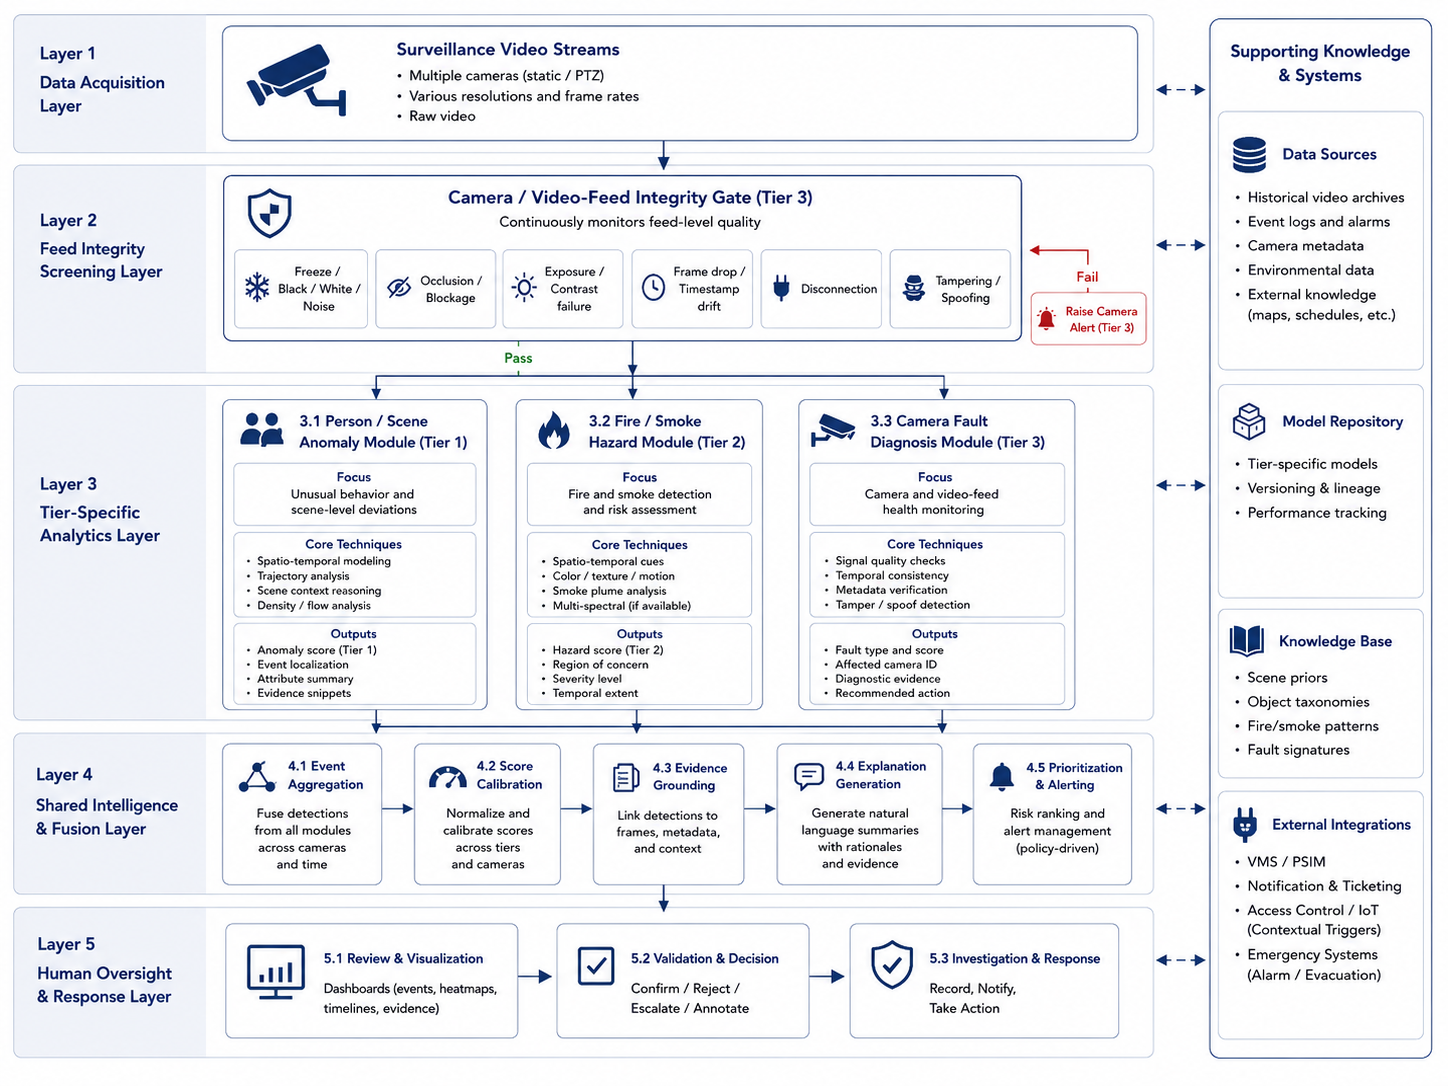
\includegraphics[width=\textwidth]{Deployment-oriented modular surveillance architecture.png}
\caption{Deployment-oriented modular surveillance architecture. Feed-integrity gating protects downstream analysis; behavioral, hazard, and feed-diagnosis modules retain task-appropriate evidence; and a shared event, calibration, evidence, and human-oversight layer supports auditable operation and controlled adaptation.}
\label{fig:modular_deployment}
\end{figure*}

Table~\ref{tab:challenges_summary} provides a structured summary linking each identified open challenge to the most promising future research directions.


\begin{table*}[!t]
\centering
\caption{Summary of open challenges and corresponding future research opportunities for visual anomaly detection in surveillance.}
\label{tab:challenges_summary}
\renewcommand{\arraystretch}{1.35}
\resizebox{\textwidth}{!}{%
\begin{tabular}{p{4.5cm}p{5.5cm}p{4.0cm}p{3.5cm}}
\toprule
\textbf{Open Challenge} & \textbf{Current Limitation} & \textbf{Promising Direction} & \textbf{Key Enabler} \\
\midrule
Anomaly definition ambiguity & Context-dependent, subjective, open-set nature of anomalies & Foundation model + natural language anomaly specification & VLMs, prompt engineering \\
\midrule
Domain generalization & Performance degradation across camera sites and environments & Meta-learning, domain adaptation, FM zero-shot transfer & Large-scale pretraining, few-shot learning \\
\midrule
Concept drift & Model degradation over time due to evolving normality & Continual learning, online adaptation, adaptive baselines & Experience replay, modular adapters \\
\midrule
Real-time edge deployment & High latency of transformers and FMs on edge hardware & Efficient architectures, model compression, NAS & Linear attention, Mamba, quantization \\
\midrule
Anomalous data scarcity & Class imbalance; limited anomaly diversity in training sets & Synthetic data generation via diffusion models and GANs & Controllable video generation \\
\midrule
Spatiotemporal localization & Coarse frame-level outputs; lack of pixel-level datasets & Pixel-level architectures, virtual annotated datasets & UBnormal-style synthetic data \\
\midrule
Interpretability & Black-box deep models undermine operator trust & Attention visualization, VLM natural language explanations & XAI integration, human-in-loop \\
\midrule
Privacy and ethics & Identity exposure, algorithmic bias, regulatory compliance & Federated learning, skeleton/flow representations, on-device processing & EU AI Act, differential privacy \\
\midrule
Adversarial robustness & No threat models, attack benchmarks, or validated defenses for VAD & Adversarial evaluation tracks; robust training for one-class/MIL formulations & Adversarial ML toolchains, red-teaming \\
\midrule
Unified multi-category detection & Fragmented methods for behavior, fire, camera anomalies & Modular or open-vocabulary architecture with tier-specific validation & Open-vocabulary VLMs \\
\midrule
Evaluation standardization & Incompatible protocols across anomaly categories and tasks & Unified benchmarks, leaderboards, reproducibility standards & Community-driven challenge design \\
\midrule
Context-aware reasoning & Lack of compositional, rule-based scene understanding & Neuro-symbolic architectures, scene graphs, temporal logic & Differentiable logic, knowledge graphs \\
\bottomrule
\end{tabular}%
}
\end{table*}


\subsection{Critical Synthesis: What the Operational Framework Reveals}
\label{subsec:critical_synthesis}

Beyond cataloging methods and identifying gaps, the operational framework enables several non-obvious comparative insights that merit explicit articulation.

\subsubsection{Five Falsifiable Cross-Tier Transfer Hypotheses}
\label{subsubsec:hypotheses}

The central analytical claim of the framework is that cross-category transferability is \emph{asymmetric}: the mechanism that ports most readily is determined by whether the source anomaly score encodes an assumption the target tier satisfies, not by how mature the source tier is. Because no controlled cross-tier experiment exists in the reviewed literature, this claim cannot be reported as a finding. We therefore state it as five numbered hypotheses, each paired with the measurement that would falsify it, so that the transfer roadmap of Table~\ref{tab:transfer_roadmap} becomes an executable research agenda rather than an expression of expectation. Each hypothesis is falsifiable in the strict sense: a stated observation would refute it.

\begin{description}[leftmargin=2.6em,style=nextline]
\item[\textbf{H1 (Reconstruction transfers to feed integrity).}] A reconstruction or feature-prediction model whose representation is made sensitive to blur, exposure, compression, and viewpoint drift, and whose normality baseline is re-estimated per camera and updated online, will detect tampering and gradual degradation at a lower false-alarm rate per camera hour than a static per-camera image-quality threshold, on unseen cameras and across a day--night and seasonal split. \emph{Refuted if} the adapted reconstruction model does not improve on the NR-IQA threshold baseline at matched detection delay, or if its advantage disappears on cameras held out from baseline estimation.
\item[\textbf{H2 (Self-supervised pretexts transfer to feed integrity).}] Pretext tasks that decouple scene change from feed failure---blur-level, exposure, compression-artifact, and frame-order prediction---will yield representations that separate genuine feed faults from legitimate scene change more reliably than pretexts defined over motion and appearance semantics. \emph{Refuted if} a motion-centric self-supervised encoder matches the quality-sensitive one on real and synthetic fault trajectories under an unseen-camera protocol.
\item[\textbf{H3 (Feature-magnitude MIL does \emph{not} transfer to early smoke).}] Weakly supervised objectives that rank temporal instances by feature magnitude will underperform on diffuse, low-contrast early smoke relative to the same supervision paired with regional photometric and temporal evidence, because the ranking objective presupposes a magnitude response that early smoke does not produce. \emph{Refuted if} an unmodified feature-magnitude MIL detector attains comparable smoke-only recall and early-event latency to the regionally supervised variant at a matched operating point.
\item[\textbf{H4 (Vision-language transfer to hazards requires temporal aggregation and calibration, not vocabulary).}] The limiting factor for open-vocabulary fire and smoke detection is not the availability of a text-specified category but temporal aggregation, small-region grounding, and calibrated abstention; supplying finer combustion prompts alone will not close the early-detection gap. \emph{Refuted if} prompt refinement alone, holding aggregation and calibration fixed, recovers the early-smoke latency and false-alarm performance of a task-specific detector on cross-weather and day--night test sets.
\item[\textbf{H5 (No single learned model is currently reliable across all three tiers).}] Under one common training and evaluation protocol, a single architecture will not match tier-specialized modules simultaneously on behavioral event detection, early hazard warning, and feed-integrity monitoring, when each is scored with its own task-appropriate operational metric. \emph{Refuted if} a unified model matches or exceeds the modular composition of Figure~\ref{fig:modular_deployment} on all three tiers under a shared protocol and shared operating-point selection.
\end{description}

H1 and H2 are the transfer directions for which adjacent-domain evidence already exists; H3 and H4 are the directions the reviewed evidence suggests are obstructed; H5 is the negative claim that the modular architecture of Section~\ref{subsec:cross_category} is proposed to test rather than to assume. All five require controlled cross-tier experiments and are offered to guide, not to substitute for, empirical validation.

\subsubsection{What the Protocol-Aware Reading Changes}

\textbf{Benchmark saturation obscures real progress.} Performance on UCSD Ped2 has effectively saturated (multiple methods exceed 97\% AUC), yet this dataset's single-scene, narrow-anomaly design means that gains above 95\% may reflect overfitting to dataset-specific artifacts rather than genuine anomaly detection improvement. Continued reliance on Ped2 can overstate practical progress when gains are not confirmed on multi-scene or cross-dataset protocols. More critically, the reported gap between the original MIL baseline and selected CLIP-based methods on UCF-Crime (75.4\% to 88.0\%) is more informative about the evolution of weakly supervised protocols than the sub-point differences on Ped2, because UCF-Crime's diverse, untrimmed, multi-category videos better approximate operational conditions.

\textbf{Foundation model gains are genuine but narrowly validated.} The strong literature-reported performance of selected CLIP-based methods on UCF-Crime and XD-Violence is driven by their ability to leverage \emph{semantic category labels} during inference, a capability that earlier fixed-label pipelines do not provide in the same form. However, these gains have been validated almost exclusively on weakly supervised benchmarks with categorical anomaly labels that align well with CLIP's text-image alignment. Whether foundation models can detect \emph{contextual} anomalies (e.g., a person running in a hospital corridor vs.\ a park) or \emph{gradual} anomalies (e.g., progressive camera defocus) with equal effectiveness remains undemonstrated.

\textbf{The deployment gap is not just computational.} Discussions of deployment readiness typically focus on inference latency, but our synthesis suggests that \emph{domain shift} is at least as important as computational cost. Methods that achieve high AUC on single-scene benchmarks can degrade substantially when transferred to unseen scenes without adaptation, as illustrated by scene-adaptation and cross-dataset studies~\citep{lu2020few}; existing benchmarks capture this only partially: multi-scene collections such as ShanghaiTech, NWPU Campus, and UBnormal~\citep{luo2017revisit, cao2023nwpu, acsintoae2022ubnormal} mix scenes within a single protocol but do not enforce a train-on-scene-A, test-on-scene-B evaluation. The mismatch between benchmark protocols and operational reality means that the field's strongest published claims may not survive deployment.


\subsection{What This Review Adds to Existing Research}
\label{subsec:what_this_adds}

Relative to the surveys compared in Table~\ref{tab:survey_comparison}, this review makes five contributions that are methodological as well as topical. We state them explicitly so that the incremental claim can be checked against the prior literature rather than inferred from coverage breadth.

\emph{First, a surveillance-specific operational taxonomy that admits feed integrity as a co-equal analytical tier.} Prior surveillance reviews treat camera and video-feed failure either as out of scope or as an engineering concern adjacent to the research problem; the narrow reviews that do address it~\citep{mantini2023feature_survey} do not place it alongside behavioral and hazard detection under a common analytical treatment. Admitting it as Tier~3 is not a coverage decision but an analytical one: it is what makes the evidence asymmetry across tiers measurable, and Table~\ref{tab:evidence_maturity} is the instrument that measures it. We do not claim equal evidence volume across tiers---the central finding is precisely that the evidence is markedly asymmetric.

\emph{Second, separable rather than collapsed method dimensions.} Existing reviews organize the literature by model family, so that a paper is resolved into exactly one bin (CNN-based, transformer-based, generative). That convention makes it structurally impossible to ask whether a reported gain is attributable to supervision, to backbone, or to pretraining scale. By coding supervision regime, anomaly-scoring mechanism, and representation family as independently assignable dimensions (Table~\ref{tab:orthogonal_coding}), the review can separate these attributions, and Section~\ref{subsec:consolidated} uses that separation to identify the pretraining/backbone confound underlying the most frequently cited performance gap in the weakly supervised literature.

\emph{Third, a protocol-aware comparability procedure applied consistently rather than declared.} The decision rule of Figure~\ref{fig:comparability_tree} is executed against every comparison table in the review, and its verdicts are recorded as per-row appraisal flags. The consequence is reported rather than hidden: almost every cross-row pair in Tables~\ref{tab:consolidated_performance} and~\ref{tab:weak_foundation_performance} qualifies only for qualified comparison, which is why no global ranking appears anywhere in this article. Reviews that tabulate the same numbers without applying such a rule implicitly present them as a leaderboard.

\emph{Fourth, cross-tier transfer stated as falsifiable hypotheses rather than as expectation.} The five hypotheses of Section~\ref{subsubsec:hypotheses} each name the experiment that would refute them and the operational metric that experiment must report. To our knowledge no prior surveillance survey states its transfer claims in a form that a subsequent primary study could disconfirm.

\emph{Fifth, systematic documentation of what the primary literature fails to report.} Section~\ref{subsec:threats_studies} records that variance information, cross-scene protocols, and operating-point reporting are absent from the majority of studies and nearly absent from the feed-integrity tier. We frame this not as a limitation encountered by the review but as a substantive finding about the field's developmental stage: the reporting practices currently in use cannot support the deployment claims the field makes, and the reporting requirements of Section~\ref{subsec:future_opportunities} follow from that finding rather than from methodological preference.

\subsection{Limitations of the Reviewed Studies}
\label{subsec:threats_studies}

The limitations in this subsection are properties of the primary literature rather than of the present synthesis. They constrain what any review of this evidence base could conclude, and each corresponds to a dimension of the appraisal instrument of Section~\ref{subsubsec:appraisal}.

\textbf{Protocol heterogeneity and non-commensurable reporting (D3, D4).} Literature-reported numbers differ in supervision, backbone, pretraining, modality, split, preprocessing, temporal smoothing, and evaluation implementation. Fire/smoke work reports classification accuracy, detection mAP, and segmentation mIoU under study-specific thresholds; feed-integrity work reports EER and decision delay under per-camera baselines. These quantities do not answer the same question and cannot be placed on a common scale, which is the proximate reason no pooled estimate is computed anywhere in this review (Section~\ref{subsec:synthesis_logic}).

\textbf{Absence of variance information (D3).} Benchmark papers overwhelmingly report a single point value on a fixed public split, without repeated runs, seeds, or confidence intervals. Consequently the field cannot distinguish a genuine improvement from run-to-run variation, and small reported margins on saturated benchmarks such as UCSD Ped2 carry no demonstrated statistical content.

\textbf{Duplicate and non-independent experimental evidence (D2).} Conference papers, journal extensions, codebases, and follow-up analyses frequently reuse the same dataset, feature extractor, or experiment, and legacy baseline values are commonly transcribed from one comparative table into the next rather than reproduced. Such evidence is not statistically independent. Superseded reports are consolidated where identifiable, and venue/version relationships are recorded in the evidence table, but residual duplication is unavoidable.

\textbf{Benchmark reuse and pretraining contamination (D2, D5).} Repeated tuning on canonical datasets can produce benchmark-specific overfitting even without explicit train--test leakage. Web-scale foundation models may additionally have encountered benchmark frames, captions, or near-duplicates during pretraining, making some zero-shot claims difficult to interpret. Current publications rarely provide contamination audits, so foundation-model generalization should be regarded as incompletely identified.

\textbf{Single-protocol external validity (D5).} As reported in Section~\ref{subsec:consolidated}, none of the tabulated normal-only results reports a train-on-scene-A/test-on-scene-B protocol, and operational reporting---latency, throughput, false alarms per camera hour, detection delay---is absent from the majority of studies and almost entirely absent from the feed-integrity tier. The field's headline numbers are therefore in-distribution by construction, and deployment readiness cannot be assessed from them.

\textbf{Reporting-practice deficiency as a substantive finding.} We emphasize that the preceding items are not merely obstacles encountered by this review. That a mature, high-volume subfield systematically omits variance, cross-scene evaluation, and operating-point reporting is itself a result about the field's developmental stage, and it is the reason the reporting requirements of Section~\ref{subsec:future_opportunities} are framed as a community obligation rather than as advice.

\subsection{Limitations of This Review}
\label{subsec:threats_review}

\textbf{Search completeness and database coverage.} The review used five broad literature sources, tier-specific vocabulary, citation tracking, and a 2026 proceedings update. Non-English studies, poorly indexed venues, papers using unexpected terminology, and work outside the selected databases may nevertheless have been missed. Google Scholar was used only for supplementary discovery because its ranking, personalization, and Boolean behavior are not fully reproducible. Terminology in the feed-integrity tier is especially unstable---camera health, camera integrity, tampering detection, and video quality diagnosis all denote overlapping problems---so despite the dedicated query family of Table~\ref{tab:query_families} the recall of that tier is the least assured of the three.

\textbf{Protocol registration.} The review protocol was specified before the final search was executed but was not prospectively registered in an external registry. The protocol and amendment history should be retained with the replication materials so that post-specification changes remain auditable. PROSPERO was not used because this methodological computer-vision review falls outside its health-review scope. Any later public deposit should be described accurately as a retrospective deposit of the pre-existing protocol, not as prospective registration.

\textbf{Two-author review team.} Both authors screened and appraised independently and agreement statistics are reported in Section~\ref{subsec:study_selection}, but with a two-person team there was no third rater available to adjudicate residual disagreements, which were instead resolved by discussion. Discussion-based resolution can in principle converge on a shared bias that a third adjudicator would have detected. The full independent decision sets are released so that a reader may recompute agreement and inspect the resolved cases directly.

\textbf{Evidence-selection and coding subjectivity.} Borderline scope, direct-transfer relevance, maturity labels, and transfer hypotheses require author judgment. The coding manual separates supervision, scoring, representation, output, and deployment, but reasonable reviewers may code hybrid systems differently, and the maturity thresholds of Section~\ref{subsec:evidence_maturity}, while predeclared, are ordinal judgments about evidence infrastructure rather than measurements. The supplementary extraction table retains decision notes and flags rather than hiding these judgments in aggregate scores.

\textbf{Language, venue, and publication bias.} English-language and peer-reviewed publication criteria can exclude relevant technical reports and regional research. Positive results are more likely to be published than failed replications, and main-conference, findings, workshop, and arXiv evidence differ in review depth. Publication category is therefore recorded and emerging evidence is not used alone to establish benchmark leadership. We note that because no effect size is pooled, the standard quantitative diagnostics for publication bias---funnel-plot asymmetry, Egger's regression, selection models---are not applicable here; the bias is acknowledged and mitigated by design rather than estimated.

\textbf{Transcription risk.} Manual transfer of results between publications and this manuscript can introduce transcription or attribution errors. Every numerical manuscript entry is linked to a provenance row in Supplementary Material~S4 and subjected to automated consistency checks, but readers should still consult the original paper for decisive comparisons.

\textbf{Rapid publication cycle.} The evidence freeze is 30 June 2026. Official WACV/CVPR main, findings, and workshop papers available by that date are coded separately, while later publications and revised versions may alter the landscape.

\textbf{Taxonomy scope.} The twelve core subcategories were selected for operational coherence and comparable evidence. Flooding, explosions, illumination transitions, mobile-camera regimes, industrial inspection, and medical anomaly detection require additional branches or dedicated reviews. Evidence-maturity labels and the transfer hypotheses H1--H5 are not effect-size estimates and require controlled cross-tier experiments and future benchmark validation.

\section{Conclusion}
\label{sec:conclusion}

This systematic review, conducted under a protocol specified before the final search and reported following PRISMA~2020, has examined visual anomaly detection across behavioral/object-interaction events, fire and smoke hazards, and camera/video-feed-integrity failures. Its principal contribution is an operational framework that separates anomaly tier from supervision regime, scoring mechanism, representation family, output granularity, and deployment profile, so that weak supervision, reconstruction, transformers, and foundation-model pretraining are not treated as mutually exclusive method categories.

Three findings merit emphasis. First, behavioral VAD has the deepest benchmark and method ecosystem, but frame-level AUC saturation on early datasets does not establish event-level or cross-scene reliability. Second, fire/smoke recognition has strong task-specific detectors but fragmented classification, detection, segmentation, and early-warning protocols. Third, camera/feed integrity is a prerequisite for trustworthy downstream analytics yet remains weakly standardized, particularly for gradual degradation, transport faults, cross-camera generalization, false alarms per camera hour, and detection delay.

Foundation and multimodal models expand anomaly vocabulary and operator-facing description, but their benefits depend on training information, prompt design, temporal aggregation, grounding, calibration, and explanation faithfulness. The next stage of progress should prioritize event-centric and low-FPR evaluation, cross-dataset generalization, adaptive normality under drift, efficient causal inference on edge hardware, robust and privacy-preserving representations, and modular multi-tier systems that preserve task-appropriate metrics. The review's transfer roadmap is therefore a set of testable research hypotheses, not a substitute for empirical transfer studies.

\section*{Declarations}
\addcontentsline{toc}{section}{Declarations}

\textbf{Acknowledgment and Funding} This work was partially funded under the PNRR Next Generation EU (Article 8, Ministerial Decree 630/2024) and supported by the Research and Innovation Project ``IMAHS -- Intelligent Multi-agent Architecture for Himalaya Supervisor'', funded through Public Intervention 1.1.1.1 of the Abruzzo Regional Programme ERDF 2021--2027 (RIS3 Abruzzo 2021--2027). The research was carried out in collaboration with SPEE Srl, L'Aquila, Italy, under the supervision of Professor Giovanni De Gasperis at the University of L'Aquila.

% AUTHOR CHECK BEFORE SUBMISSION: confirm and state the role of the funders/sponsors if applicable.
\textbf{Competing interests} The authors declare no competing interests.

\textbf{Author contributions} Tayyab Rehman: conceptualization, literature search, evidence synthesis, visualization, and writing--original draft. Giovanni De Gasperis: supervision, methodology review, validation, and writing--review and editing. Both authors approved the final manuscript.

\textbf{Data availability} No new visual or video dataset was generated. The review is based on publicly available publications and benchmark descriptions cited in the manuscript. Supplementary Materials S1--S5 accompany the submission: database-specific search specifications and evidence-freeze log; citation inventory; core primary-evidence extraction table; numerical performance-provenance table; and validation/table-generation scripts with a data dictionary, checksums, amendment log, and audit report. The replication package (search specifications, citation inventory, evidence-extraction and performance-provenance tables, and validation scripts) is publicly available at \url{https://github.com/tayyabrehman96/From-Scene-Events-to-Video-Feed-Failures}.

\textbf{Code availability} No new detection model is introduced. Scripts that validate the review data and regenerate data-derived summary tables are included in Supplementary Material~S5 and in the public repository at \url{https://github.com/tayyabrehman96/From-Scene-Events-to-Video-Feed-Failures}.

\textbf{Declaration on Generative AI} The scientific ideas, evidence selection, interpretations, and conclusions remain the responsibility of the human authors. Generative AI tools were used during manuscript revision for language editing, structural review, and drafting assistance. The authors critically reviewed, fact-checked, and approved all retained text and remain fully accountable for the accuracy, originality, citations, and integrity of the final manuscript. Generative AI is not listed as an author.


%% ============================================================
%%  APPENDICES (reproducibility)
%% ============================================================
\appendix

\section{Executable Database Search Strings}
\label{app:search_strings}
To make the search specification reproducible from within the manuscript itself (rather than only through Supplementary Material~S1), we provide the full, executable Boolean strings used at each fielded database. Field codes and date filters are shown as applied; the four concept blocks correspond to the query families of Table~\ref{tab:query_families}. Google Scholar was queried only for supplementary discovery and its non-fielded phrase queries are archived in S1.

\paragraph{Scopus (\texttt{TITLE-ABS-KEY}).}
\begin{small}
\begin{verbatim}
TITLE-ABS-KEY(
 ("video anomaly detection" OR "abnormal event" OR "anomalous event"
  OR "violence detection" OR loitering OR "fall detection"
  OR "crowd anomaly" OR "traffic anomaly" OR "abandoned object")
 OR ( (fire OR flame OR smoke OR wildfire OR haze) W/5
      (detection OR classification OR segmentation OR "early warning") )
 OR ( ("camera tampering" OR "camera anomaly" OR "lens occlusion"
       OR "defocus" OR "frozen stream" OR "frame loss"
       OR "signal corruption" OR "no-reference image quality") )
)
AND ( surveillance OR CCTV OR "closed-circuit" OR monitoring
      OR "traffic camera" )
AND ( "deep learning" OR CNN OR RNN OR autoencoder OR transformer
      OR "vision-language" OR "foundation model" OR "self-supervised"
      OR "multiple instance" OR diffusion OR "state-space" OR Mamba )
AND PUBYEAR > 2009 AND PUBYEAR < 2027
AND ( LIMIT-TO(DOCTYPE,"ar") OR LIMIT-TO(DOCTYPE,"cp") )
AND ( LIMIT-TO(LANGUAGE,"English") )
\end{verbatim}
\end{small}

\paragraph{Web of Science Core Collection (Topic field \texttt{TS}).}
\begin{small}
\begin{verbatim}
TS=( ("video anomaly detection" OR "abnormal event" OR "anomalous event"
      OR "violence detection" OR loitering OR "fall detection"
      OR "crowd anomaly" OR "traffic anomaly" OR "abandoned object"
      OR (fire OR flame OR smoke OR wildfire) NEAR/5
         (detection OR classification OR segmentation)
      OR "camera tampering" OR "camera anomaly" OR "lens occlusion"
      OR "frozen stream" OR "frame loss" OR "no-reference image quality") )
AND TS=( surveillance OR CCTV OR "closed-circuit" OR monitoring )
Refined by: Document Types = (ARTICLE OR PROCEEDINGS PAPER)
            Languages = (ENGLISH)
Timespan = 2010-01-01 to 2026-06-30
\end{verbatim}
\end{small}

\paragraph{IEEE Xplore (Command Search; metadata + abstract).}
\begin{small}
\begin{verbatim}
( "All Metadata":"video anomaly detection" OR "abnormal event"
  OR "violence detection" OR "crowd anomaly" OR "abandoned object"
  OR "fire detection" OR "smoke detection" OR "camera tampering"
  OR "camera anomaly" OR "frozen stream" OR "frame loss" )
AND ( "All Metadata":surveillance OR CCTV OR monitoring )
AND ( "All Metadata":"deep learning" OR CNN OR transformer
      OR autoencoder OR "vision-language" OR "self-supervised"
      OR "multiple instance" )
Filters: Year 2010-2026; Content Type: Conferences, Journals
\end{verbatim}
\end{small}

\paragraph{ACM Digital Library (Advanced Search; title/abstract/keywords).}
\begin{small}
\begin{verbatim}
[[Title: "video anomaly detection"] OR [Abstract: "abnormal event"]
 OR [Keywords: "violence detection"] OR [Abstract: "fire detection"]
 OR [Abstract: "smoke detection"] OR [Abstract: "camera tampering"]]
AND [[Abstract: surveillance] OR [Abstract: CCTV]
     OR [Abstract: monitoring]]
AND [Publication Date: (01/01/2010 TO 06/30/2026)]
\end{verbatim}
\end{small}

\noindent The official WACV~2026 and CVPR~2026 open-access proceedings were additionally screened title-by-title against the same vocabulary before the 30~June~2026 evidence freeze, with the main/findings/workshop designation recorded per item (Section~\ref{subsec:search_strategy}).

\section{PRISMA 2020, PRISMA-S, and SWiM Reporting Checklists}
\label{app:prisma2020}
Table~\ref{tab:prisma_map} maps relevant PRISMA~2020 items~\citep{page2021prisma}, PRISMA-S search-reporting items~\citep{rethlefsen2021prismas}, and the nine SWiM reporting items~\citep{campbell2020swim} to the manuscript. SWiM is used here as an adapted transparency framework for a non-pooled synthesis; its intervention-effect terminology is interpreted cautiously in the context of heterogeneous computer-vision benchmark evidence. Any item that depends on record-level screening data must be completed from the underlying ledger and independent reviewer files before the manuscript is described or submitted as a systematic review.

\begin{small}
\begin{longtable}{@{}p{0.44\linewidth}p{0.50\linewidth}@{}}
\caption{Reporting-checklist mapping.}\label{tab:prisma_map}\\
\toprule
Item & Location / status \\
\midrule
\endfirsthead
\toprule Item & Location / status \\ \midrule \endhead
\multicolumn{2}{@{}l}{\textit{PRISMA 2020}}\\
Title identifies the report as a systematic review & Title \\
Structured abstract & Abstract \\
Rationale and objectives & Section~\ref{sec:introduction} \\
Eligibility criteria & Table~\ref{tab:eligibility} \\
Information sources & Section~\ref{subsec:search_strategy}; Table~\ref{tab:search_reporting} \\
Full search strategies for all sources & Appendix~\ref{app:search_strings}; Supplementary~S1 \\
Selection process (independent screening, $\kappa$) & Section~\ref{subsec:study_selection}: \pnum{$\kappa=0.754/0.877$}; raw agreement \pnum{97.0\%/94.6\%} \\
Data collection process and data items & Section~\ref{subsec:study_selection}; Supplementary~S3 \\
Risk-of-bias / quality assessment & Section~\ref{subsubsec:appraisal}; instrument in Table~\ref{tab:appraisal_instrument}; per-study consensus ratings in Appendix~\ref{app:appraisal} and S3 \\
Synthesis methods & Section~\ref{subsec:synthesis_logic}; Figure~\ref{fig:comparability_tree} \\
Reporting-bias assessment & Sections~\ref{subsec:threats_studies} and~\ref{subsec:threats_review} \\
Study-selection flow with reasons for exclusion & Figure~\ref{fig:prisma}: \pnum{$N_1=16{,}482$, $N_5=616$} \\
Study characteristics & Tables~\ref{tab:sota_person}--\ref{tab:sota_camera}; Supplementary~S3 \\
Results of syntheses & Sections~\ref{sec:sota}--\ref{sec:datasets} \\
Certainty of evidence & No formal GRADE-style certainty assessment was applied; Table~\ref{tab:evidence_maturity} reports evidence-infrastructure maturity, not certainty of an intervention effect \\
Limitations & Section~\ref{subsec:threats_studies} (reviewed studies); Section~\ref{subsec:threats_review} (this review) \\
Registration and protocol & Section~\ref{subsec:threats_review}: protocol specified before the final search but not prospectively registered; any later public deposit must be labelled retrospective; PROSPERO not used (out of scope) \\
Support / competing interests & Declarations \\
Data, code and materials availability & Declarations; Supplementary~S1--S5 \\
\midrule
\multicolumn{2}{@{}l}{\textit{PRISMA-S (search reporting)}}\\
Database name and platform & Section~\ref{subsec:search_strategy}; Table~\ref{tab:search_reporting} \\
Full Boolean search strings & Appendix~\ref{app:search_strings}; Supplementary~S1 \\
Date of search / evidence freeze & Section~\ref{subsec:search_strategy} (freeze 30 June 2026) \\
Limits and restrictions & Appendix~\ref{app:search_strings}; Table~\ref{tab:eligibility} \\
Field labels and syntax per database & Appendix~\ref{app:search_strings} \\
Supplementary and grey-source strategy & Section~\ref{subsec:search_strategy} \\
Citation chasing (backward/forward) & Section~\ref{subsec:search_strategy} \\
Deduplication method & Section~\ref{subsec:search_strategy}: two-pass (DOI, then normalised title/author/year), then manual residual review \\
Number of records at each stage & Figure~\ref{fig:prisma}: all identification, screening, eligibility, and inclusion counts shown \\
Peer review of the search strategy & \ptext{No formal librarian/information-specialist peer review is assumed in this working draft; verify this statement before submission. The strategy was developed and cross-checked by both authors.} \\
\midrule
\multicolumn{2}{@{}l}{\textit{SWiM (synthesis without meta-analysis)}}\\
1. Grouping studies for synthesis & Section~\ref{subsec:synthesis_logic}: grouped by anomaly tier, then by supervision regime and task, because these determine commensurability \\
2. Standardised metric for synthesis & Not applicable: no common estimand exists across tiers or supervision regimes; rationale in Section~\ref{subsec:synthesis_logic} \\
3. Synthesis method & Structured tabulation with protocol conditions attached; comparability adjudicated by Figure~\ref{fig:comparability_tree}; no vote counting and no pooling \\
4. Criteria used to prioritise results & Section~\ref{subsec:eligibility}: peer-reviewed and main-conference evidence prioritised; 2026 findings/workshop and preprint evidence used only to characterise emerging directions \\
5. Investigation of heterogeneity & Sections~\ref{subsec:evidence_maturity} and~\ref{subsec:consolidated}: heterogeneity is treated as a protocol property and reported per row as an appraisal flag rather than estimated as a statistic \\
6. Certainty / limitations of the synthesis & Table~\ref{tab:evidence_maturity} (predeclared maturity criteria); Sections~\ref{subsec:threats_studies} and~\ref{subsec:threats_review} \\
7. Data presentation methods & Tables~\ref{tab:consolidated_performance} and~\ref{tab:weak_foundation_performance} present values with supervision, backbone, pretraining and modality attached; no global rank is assigned \\
8. Reporting results of the synthesis & Sections~\ref{sec:sota}--\ref{sec:datasets}; direction and certainty stated in words, with the protocol conditions under which each holds \\
9. Limitations of the synthesis approach & Section~\ref{subsec:threats_review}: without pooling, quantitative publication-bias diagnostics are unavailable and no effect magnitude is estimated \\
\bottomrule
\end{longtable}
\end{small}

\section{Per-Study Critical Appraisal Ratings}
\label{app:appraisal}

Table~\ref{tab:appraisal_ratings} is the submission-format location for the consensus rating of each core primary study on the five appraisal dimensions defined in Table~\ref{tab:appraisal_instrument}. Ratings are \textbf{L} (low concern), \textbf{S} (some concerns), and \textbf{H} (high concern). Both authors rated every study independently; the agreement statistics are given in Section~\ref{subsubsec:appraisal}. \ifprovisionalnumbers The individual S3 rating rows were not available in the supplied manuscript package and therefore are intentionally not fabricated here; they must be inserted from the original appraisal file before submission. \else The two independent rating sets are supplied in Supplementary Material~S3 so that the consensus values can be recomputed. \fi No study is excluded on the basis of its rating, and no row total or composite score is computed: the columns are diagnostic and are not commensurable with one another.

The distribution is itself informative and should be read alongside Section~\ref{subsec:threats_studies}. Concentrations of \textbf{H} in D4 and D5 are expected and reflect a field-level convention---reporting a single in-distribution split against baselines that differ in backbone and pretraining---rather than deficiencies peculiar to individual papers. Where a rating materially changes how a tabulated number should be read, that consequence is stated at the point of use rather than left to this appendix.

\begin{small}
\begin{longtable}{@{}p{0.30\linewidth}p{0.10\linewidth}ccccc@{}}
\caption{Per-study consensus appraisal ratings. D1 experimental transparency; D2 dataset/split integrity; D3 metric validity; D4 comparison fairness; D5 external validity. L = low concern, S = some concerns, H = high concern.}\label{tab:appraisal_ratings}\\
\toprule
Study & Tier & D1 & D2 & D3 & D4 & D5 \\
\midrule
\endfirsthead
\toprule Study & Tier & D1 & D2 & D3 & D4 & D5 \\ \midrule \endhead
\multicolumn{7}{@{}p{0.96\linewidth}@{}}{\ptext{AUTHOR VERIFICATION REQUIRED: the manuscript working total is 132 core studies, but individual D1--D5 consensus ratings cannot be reconstructed from the manuscript or bibliography alone. Populate these rows directly from the original S3 appraisal file before setting \texttt{\string\provisionalnumbersfalse}.}}\\
\bottomrule
\end{longtable}
\end{small}

\section{Reproducibility Statement}
\label{app:repro_statement}
The intended versioned replication package (Supplementary~S1--S5) comprises database-specific query specifications and the evidence-freeze log (S1); the bibliographic citation inventory (S2); the core primary-evidence extraction table with per-row appraisal flags (S3); the numerical performance-provenance table linking every reproduced figure to its immediate source (S4); and validation/table-generation scripts, a data dictionary, checksums, amendment log, and audit report (S5). \ifprovisionalnumbers\textbf{Author verification required: S1--S5 were not present in the manuscript files supplied for this revision, so the claims in this paragraph must be checked against the actual supplementary package before submission.}\else The scripts validate required fields, duplicate keys, dataset/metric label consistency, and manuscript-table coverage so that data-derived summary tables regenerate without manual transcription. The package additionally contains the raw database exports, deduplication log, and both screeners' independent decisions, allowing the PRISMA flow and reported $\kappa$ values to be recomputed from source.\fi

%% ============================================================
%%  BIBLIOGRAPHY
%% ============================================================
% REFERENCE STYLE. Artificial Intelligence Review uses Springer's name-year style.
% For submission, download the AIR / Springer Nature LaTeX pack and use:
%   \bibliographystyle{spbasic}      (svjour3 pack)   -- or --
%   \bibliographystyle{sn-basic}     (sn-jnl pack)
% abbrvnat below is the closest style present in a stock TeX Live install and is
% used here only so the file compiles without the Springer pack.
\bibliographystyle{abbrvnat}
\bibliography{references}

\end{document}